%% Do not edit unless you really know what you are doing.

%% definitiu
%% data: 10/06/2005 (dd/mm/aaaa)
%%

%% ?evite
%% ?convined

%% Els teclats nederlandesos no tenen totes les lletres...

%%<!--
%%    Se podr\'ia a\~nadir un apartado con las modificaciones hechas sobre el c\'odigo del programa?
%%    O eso quedaria para las transparencias?
%%//-->
\documentclass[11pt,oneside,english]{book}%catalan]{amsbook}
\usepackage[T1]{fontenc}
\usepackage[latin1]{inputenc}
\setcounter{secnumdepth}{4}
\setcounter{tocdepth}{4}
\usepackage{amssymb}
\usepackage{amsmath}
\usepackage{graphicx}

\makeatletter
%%%%%%%%%%%%%%%%%%%%%%%%%%%%%% Textclass specific LaTeX commands.
 \numberwithin{section}{chapter}
 %\theoremstyle{plain}    
 \newtheorem{thm}{Theorem}[section]
 \numberwithin{equation}{section} %% Comment out for sequentially-numbered
 \numberwithin{figure}{section} %% Comment out for sequentially-numbered
 \usepackage{verbatim}
 %\theoremstyle{plain}
 %\theoremstyle{plain}    
 \newtheorem{algorithm}[thm]{Algorithm} %%Delete [thm] to re-start numbering
 \newtheorem{definition}[thm]{Definition}

\usepackage{babel}
\makeatother
\begin{document}
\begin{comment}
\noindent Escola Universit\`aria Polit\`ecnica\\
Universitat de Lleida\\
Enginyeria T\`ecnica Inform\`atica de Sistemes
\end{comment}
%%<!--
%%     No se como hacer que estas tres linias salgan en la parte superior izquierda de la portada
%%//-->
%%% >>>>>>>>>>>>>>>>>>>>>>>>>>>>> Comentario Ramiro (18.oct.03) >>>>>>>>>>>>>>>>>>>>>>>>>>>>>>>>>>>>>>
%%% Creo que lo he conseguido con lo que sigue. Aunque, por un extra\~no motivo, hay un salto de 
%%% linea que no s\'e controlar. Insiste.
%%% >>>>>>>>>>>>>>>>>>>>>>>>>>>>>>>>>>>>>>>>>>>>>>>>>>>>>>>>>>>>>>>>>>>>>>>>>>>>>>>>>>>>>>>>>>>>>>>>>>
%%<!--
%%     Preguntar Damia
%%//-->
\title{GnuPG Implementation \\ with Elliptic Curves}

%%\title{Implementaci\'o GNUPG \\
%%amb Corbes El$\cdot$l\'iptiques}


\author{Sergi Blanch i Torn\'e\\
~\\
~\\
Director: \\
Ramiro Moreno Chiral
~\\
~\\
~\\
~\\
~\\
v 1.0.4a\\
~\\
Documentation of the \\ EccGnuPG 0.1 branch.\\
}
%%%%%%%%%%%%%%%%%%%%%%%%%%%%%%%%%
%      Canvis de la 1.0.2 a la 1.0.3
% - S'exclou el apendix amb el c\`odi. Ha quedat desfa\c cat i es pot obtenir de la mateixa web que la documentaci\'o.
% - Correcci\'o taula comparativa Sym~Fp~F2m
%%%%%%%%%%%%%%%%%%%%%%%%%%%%%%%%%

%%%%%%%%%%%%%%%%%%%%%%%%%%%%%%%%%
%      Per a la 1.0.4
% * Documentar devilitat EccElGamal.
% - Bibliografia de la devilitat.
% * Mirar si hi ha hagut moduficación en els algorismes.
%%%%%%%%%%%%%%%%%%%%%%%%%%%%%%%%%

\maketitle
\tableofcontents{}

%%\listof{algorithm}{List of Algorithms}

%%\listoffigures


%%\chapter*{Agraiments}
\chapter*{Gratitudes}

I am specially grateful with Ramiro, he has shown me the thinks that i have capacity to do and he gives me the opportunity to see this. And also to my friends, the ones who have helped me not to stop.

For the support and help that i receive, i need to make an appointment with the people that give me a lot of help to do this project. People as: Dami\`a Castell\`a, Jose Garc\'ia, Juan Manel Gimeno, Montse Orpina, David Paniagua. Some of them with little contributions, but really effective; others with decisive contributions, that make easy to obtain the results more quickly.

To the David Shaw, Ricard de Benito, Robert J. Hansen, the ones who help me when i ask something in the developers mail list of the GnuPG. To Mikael Mylnikov, a good hacker how find some bugs and he send a really good reports and solutions.

To all the people, that i do not even know, but they share with the community the improvements done over this project.

%%<!-- 
%%     Este apartado de agradecimientos hace dias que lo empeze para no perder a nadie en la memoria.
%%     No se si puede considerar-se inadecuado, poner miembros del tribunal en los agradecimientos;
%%     mas inadecuado me parece si no estan todos los del tribunal.
%%//-->
%%% >>>>>>>>>>>>>>>>>>>>>>>>>>>>> Comentario Ramiro (22.oct.03) >>>>>>>>>>>>>>>>>>>>>>>>>>>>>>>>>>>>>>
%%% Sin importancia relevante: pon lo que quieras
%%% >>>>>>>>>>>>>>>>>>>>>>>>>>>>>>>>>>>>>>>>>>>>>>>>>>>>>>>>>>>>>>>>>>>>>>>>>>>>>>>>>>>>>>>>>>>>>>>>>>
%%% __.

\chapter{Introduction}

The modern cryptography has taken advantage of problems with a lot of centuries of existence to protect the modern communications. These problems are usually named One Way Functions (in the future OWF). With the public key cryptography, introduced by W. Diffie and M. Hellman in the year 1976, the innovation in front of symmetric cryptography is the difference and complementary key pair, in an invocate way. This explanation is if you have one key pair not equals between them and they have a complementary relation, one can decrypt the things that the other had encrypt; the fist one is named private key and it is used to decrypt and/or sign, while the other one is named public key and it is used to encrypt and/or verify a sign. The relation between the key pair (public key/private key) is invocate. Like this we can never find the paradox of two different keys, that was synonymous with regard to only one complementary key.

Previously to the appearance of the elliptic curves, the proportional relation in security terms, offered between symmetric and asymmetric key length was really hard. To offer the same strength in security terms, of a symmetric key of 128 bits into an asymmetric key we need a key over 1024 bits. With the elliptic curves, the difference is as well as 192 bits for the asymmetric key into the 128 bits of the symmetric one.

\section{Objectives}

The Elliptic Curve Cryptographic schemes are tested and cryptanalysted for a longtime. This schemes are extensions of the very known modern schemes, but the Elliptic Curve Cryptosystems are mounted over different mathematical bases and, the beginning, ECC were stronger than another modern schemes.

The ECC due to it flexibility to all knowledge attacks and it little key measure, it is the best scheme for the systems that it have hard limitations of computation and/or bandwidth. Now, this scheme is very extended over hardware systems, for example the smart-cards.

In the software implementations field this scheme has had very small expansion, and it lives in a background. For this reason, the majority of the users of the strong cryptography do not have, in their most extended softwares, of the possibility of Elliptic Curve uses.

Werner Koch began the implementation of a software, based on OpenPGP, that he should set free under GPL license, named GnuPG (Gnu Privacy Guard). This software is the free software option before the commercial software written, some years before, by Phil Zimmermann, named PGP (Pretty Good Privacy). Now, the functionalities of both softwares (GnuPG and PGP) are similar, but GnuPG do not implement any patented algorithm.

%%<!-- www.gnupg.org ... thanks:
%%    Creadores:
%%    Matthew Skala, Michael Roth, Niklas Hernaeus, R�i Guyomarch, Werner Koch. 
%%//-->

The werner's project has gone as far as its maturity as software with the stable versions 1.2.x. This software was created together the developer team: Matthew Skala, Michael Roth, Niklas Hernaeus, R\'emi Guyomarch i Werner Koch, and actually maintained by the team: David Shaw, Stefan Ballon, Timo Schulz and Werner Koch, and the contribution of the developers mail list members <gnupg-devel@gnupg.org>.

%%% >>>>>>>>>>>>>>>>>>>>>>>>>>>>> Comentario Ramiro (22.oct.03) >>>>>>>>>>>>>>>>>>>>>>>>>>>>>>>>>>>>>>
%%% Deber�s explicar aqu\'{\i} qu\'e es un sistema h\'{\i}brido: criptograf\'{\i}a de clave p\'ublica
%%%	o asim\'etrica para intercambio de claves y firma digital + criptosistemas sim\'etricos para
%%%	cifrado.
%%% >>>>>>>>>>>>>>>>>>>>>>>>>>>>>>>>>>>>>>>>>>>>>>>>>>>>>>>>>>>>>>>>>>>>>>>>>>>>>>>>>>>>>>>>>>>>>>>>>>
%%% ok.
GnuPG software offers tools of strong cryptography, over modern schemes (except patented), for example the ElGamal scheme for the cipher tool, and the DSA scheme for the sign tool. Moreover, this software has support for RSA cryptographic system and some symmetric Cryptosystems. The supported symmetric systems are: 3DES, CAST5, BLOWFISH, AES, AES192, AES256, TWOFISH. When we use this software in the cipher side, we use hybrid Cryptosystems. That is to say, the program uses a session symmetric key (default AES) and it uses public key scheme to cipher the symmetric key to all the receivers. All the public keys have a list of preferences about the symmetric algorithms to use, and hash or compression systems.

The present project implements the schemes of the public key cryptography with elliptic curves over the free software named GnuPG. The objective, at the users side (as well as the present users of GnuPG, as much as the users of another cryptographic softwares, including the new users that do not have a definitive software chosen now) is to offer the possibility to use a new strong cryptography option over elliptic curve. My option allows all people to have the robustness that this system brings to the public key Cryptosystems.

\section{Organization and Planning}

To organize and make the plannification of this project, i have divided it in two main blocks. The first one, is theory about the elliptic curves, and the second one is about the public software that we use and the union  with the own module. In this documentation the made division is the same that first division.

The organization at the project making time have one division more. To simplify the realization of one implementation like this, it is not enough to program, we need to have a background about elliptic curves, and we need an initialization in this. In the documents, we presuppose that the reader has an idea about the mathematical base over the one we move into.

In the first part, destined to learning and documenting about the characteristics and the properties of the elliptic curves, i needed four months. In this period, we did during the realization of the subject named \textit{Theory of the Information and the Codification} (\textit{TIC})\footnote{This subject not only study cryptography, but it is an important part}. At this time, i have a deep knowledge about the mathematics tools that the elliptic curves use, and the cryptographic importance of this system, now we could have to go into the search the way to realize this implementation, and with what thinks can do this.

To start a really good, competent and trusted implementation, the first step that we need to do is to search a standard. The standard we need, has been strongly cryptanalysted for the cryptographic community. What we search in this step is protect itself to the probably mistakes, because a lot of people has worked for a long time to find this. In a parallel way to this specification task, we can realize an analysis of the host program. The reason for this analysis is to find the knowledge about the functionalities and the procedures of itself in the way of module insertion task. This task needs to read a lot of programming code, and the following of the execution, but it includes the compilation steps. We can not forget the main task which is the module insertion to the program, and this includes a compilation and an explanation to the program to it have new functions.

To work in this second block of tasks, i have spent a long time of dedication, really a long time. The reason of this time, it is not a special complexity of the ask, fate because the plannification are really spacious.

There are a lot of important things in this second block: the programming language choice to use. The best options are, and they have a heavy weight: C and C++. The second language, and the object oriented programming, are apparently ideal to work with the data structures and operations that we need. With the operators overloading, we can obtain a similar code as the mathematical writing of the operations. But there are two reasons to tilt the balance to the C language. The first one is the integration of this new module in the GnuPG software, because all the codes of this program are written in this language. It is logical that the addition code will be more refined if this is clearly integrated with the environment. The second reason, is the influence of this project. The \textit{UNIX} community, and this are the expressions used in a response of a query made to the developers of the program, use this language. The C language is in the register of all the computers programmers, if we scorn this language we will exclude the community how can check the module.

Now, it only remains the third block and the last one. This block offers the tangible results, well, it makes things observables same as documentation and code. This point, is the point in which we start programming. Based on the previous blocks, the search of the standard algorithms, we could make a collection of this. But not all of this algorithms we can use, because they can not adapt to the program gratefully, and we need to make modifications over this or remake them. These modifications are always made with a lot of caution in the way of not to generate weakness because we work in a really paranoid science field. We make a compendium of algorithms because later we use them to make the source code, and we make structures in different descendant levels. This descendant levels programming are the best, the clearest and the strongest way to programming.  At this point, it only remains the programming work: the translation of the algorithmic language to the C programming language. When we finish the programming, we need to debug the source code.

To realize this last block, we planning to dedicate the last semester of the 2002/03 academic course. But the debugging and the interaction between the module and the main software make some complications to do the last tasks. These complications forced to modify the plannification and made this longer, really longer. The main reason of this delay is the insistence of the programmers manual in this program. The correction of one execution error in this long code is a strong work generally solved with tests and provoked mistakes.

\chapter{ECC}

The Elliptic Curve Cryptosystem shows a new perspective of work with the classical problems of the modern cryptography. The Elliptic Curve Cryptography expound to change the base over that the cryptosystems work.

%%% >>>>>>>>>>>>>>>>>>>>>>>>>>>>> Comentario Ramiro (22.oct.03) >>>>>>>>>>>>>>>>>>>>>>>>>>>>>>>>>>>>>>
%%% En lo que sigue hay muchos l\'{\i}os. Primero: el l\'{\i}o grupo <-> cuerpo. Brevemente: el DLP
%%%	y los protocolos criptogr\'aficos asociados (intercambio de claves Diffie--Helman, cifrado
%%%	y descifrado ElGamal) se plantean inicialmente (1976) sobre el grupo multiplicativo de un 
%%%	cuerpo finito, es decir, sobre el cuerpo, sin el 0, y con la operaci� de multiplicar. Tales
%%%	grupos $\mathbb{F}_q^*$ o $\mathbb{F}_p^*$, en el caso primo, son siempre c\'{\i}clicos.
%%%	El ECDLP se plantea sobre el grupo $E(\mathbb{F}_q)$ de puntos de ce, que, (ojo!) no siempre
%%%	es c\'{\i}clico (lo es, precisamente, cuando el ``cofactor'' es 1). Por similitud y
%%%	comodidad, se usa un subgrupo del grupo  $E(\mathbb{F}_q)$ que sea c\'{\i}clico: el que t\'u
%%%	denotas com $\langle G\rangle$, para eso hay que elegir un generador de orden ``suficientemente''
%%%	grande. Tu llamas n a ese orden y ha de ser $n\approx \# EE(\mathbb{F}_q)$. Te corrijo, en el
%%% 	siguiente p\'arrafo grupo <-> cuerpo.
%%% >>>>>>>>>>>>>>>>>>>>>>>>>>>>>>>>>>>>>>>>>>>>>>>>>>>>>>>>>>>>>>>>>>>>>>>>>>>>>>>>>>>>>>>>>>>>>>>>>>

In the modern cryptosystems emphasize the \emph{Discrete Logarithm Problem} (in the future DLP), the strength of this depends on a multiplicative group (that is to say, the field without the 0), over this group we make the cryptographic operations. These groups as $\mathbb{F}_q^*$ or $\mathbb{F}_p^*$, in the prime case, are always cyclic. We could expound the same problem over a different group that the classic cyclic group. We replace the number of the cyclic group of a subgroup of points over an elliptic curve, and this subgroup have the same properties that the first one (for example it is cyclic), we could expound the same problem over the new field. Depending on which field we make the definition, we have differences with the operations at the lowest programming level, but the operation interface as the same for all the fields.

The new group with the cryptosystem will work, it would not a multiplicative group, and the DLP have not the basic operation in the inversion of the exponentiation. At the time we base the own operations with the elliptic curves, the product of number is converted to a point addition, and the integer exponentiation is converted to point scalar multiplication. The \emph{Elliptic Curve DLP} (in the future ECDLP) is based on the OWF that says: if you have two random points of the curve, it is a really strong computable problem, how many times on of them are added to himself to obtain the other number.

The most important advantage of the ECDLP is the key size, this size is seriously reduced. This reduction is good because makes better efficiency in systems with limitations of computation and/or bandwidth. This added to a better strength and the speed up of the cryptosystem setup, contributes with a lot of flexibility to the attacks and the cryptanalysis.

\section{Introduction to Elliptic Curves}

The best way to introduce in the elliptic curves is the definition of them, so to introduce the elliptic curves we need to see their definition. But we need to define something more before it.

\begin{definition}
We can define a projective plan over a field $\mathbb{F}$ as:

Considerate the joint 
\begin{equation}
\mathbb{F}^{3}-\left\{ \left(0,0,0\right) \right\} = \mathbb{F} \times \mathbb{F} \times \mathbb{F} -\left\{ \left(0,0,0\right) \right\},
\end{equation}
 and the next equivalence relation:
\begin{equation}
\left( x,y,z\right) \sim \left( x\prime ,y\prime ,z\prime \right) \Rightarrow \exists \lambda \in \mathbb{F}^\star : x=\lambda x \prime, y=\lambda y \prime, z=\lambda z \prime
\end{equation}
This relation allows to define a quotient that we name as \emph{Projective plan}:
\begin{equation}
\mathbb{P}_{2} \left( \mathbb{F} \right) = \frac{\mathbb{F}-\left\{ \left(0,0,0\right) \right\}}{\sim}
\end{equation}
We denoted one point in the $\mathbb{P}_{2} \left( \mathbb{F} \right)$ plan as: $\left[ X:Y:Z \right]$. And the line with $Z=0$, we named it as \emph{straight line to infinite}.

We can make an application between point in the affine plan $\mathbb{A}_{2} \left( \mathbb{F} \right) = \mathbb{F}^{2}$ and the projective plan. This reciprocal correspondence is:
\begin{equation}
\begin{array}{ccc}
 & f\\
\mathbb{F}^{2} & \longrightarrow & \mathbb{P}_{2}\left(\mathbb{{F}}\right)\\
\left(x,y\right) & \longmapsto & \left[x:y:1\right]
\end{array}
\end{equation}
\begin{equation}
\begin{array}{ccc}
 & f^{-1}\\
\mathbb{P}_{2}\left(\mathbb{{F}}\right) & \longrightarrow & \mathbb{F}^{2}\\
\left[X:Y:Z\right] & \longmapsto & \left\{ \begin{array}{ccc}
\left(\frac{X}{Z},\frac{Y}{Z}\right) & if & Z\neq0\\
\neg\exists & if & Z=0\end{array}\right.
\end{array}
\end{equation}

It is an evidence, that the projective straight line to infinite does not exist in the affine plan. And also, if we like to write an affine expression to projective coordinates, we can substitute:
\begin{equation}
\begin{array}{ccc}
x & \longmapsto & \frac{X}{Z}\\
y & \longmapsto & \frac{Y}{Z}
\end{array}
\end{equation}

We remove the divisors and reciprocally, we can write a projective expression to affine coordinates, dividing it to the maximum power of $Z$ and then substituting:
\begin{equation}
\begin{array}{ccc}
\frac{X}{Z} & \longmapsto & x\\
\frac{Y}{Z} & \longmapsto & y
\end{array}
\end{equation}

\end{definition}

\begin{definition}\label{eq:corba}
Given an elliptic curve $E/\mathbb{F}$ in $\mathbb{P}_{2}\left(\mathbb{{F}}\right)$ with the Weierstrass Normal Form (WNF)
\begin{equation}
F\left(X,Y,Z\right)=Y^{2}Z+a_{1}XYZ+a_{3}YZ^{2}-X^{3}-a_{2}X^{2}Z-a_{4}XZ^{2}-a_{6}Z^{3},

\end{equation}
with $a_{1},\ldots,a_{6}\in\mathbb{F}$ and without singular points, that is to say, such as the equation system:
\begin{equation}
\left.\begin{array}{c}
\frac{\partial F\left(X,Y,Z\right)}{\partial X}=0\\
\frac{\partial F\left(X,Y,Z\right)}{\partial Y}=0\\
\frac{\partial F\left(X,Y,Z\right)}{\partial Z}=0\\
F\left(X,Y,Z\right)=0\end{array}\right\}
\end{equation}
does not have solution.
\end{definition}

The definition \ref{eq:corba} describes the general equation of an elliptic curve, but when we define an elliptic curve to describe the cryptosystem setup, we use the reduced form.

\begin{definition}
If the characteristic of the $\mathbb{F}$ is not $2$ or $3$ the WNF equation can be reduced to:
\begin{equation}
Y^{2}Z=X^{3}+aXZ^{2}+bZ^{3}
\label{eq:reduida}
\end{equation}
and we can change the no-singularity condition to the equivalent like:
\begin{equation}
\Delta=-\left(4a^{3}+27b^{2}\right)\neq0
\end{equation}
The \ref{eq:reduida} curve cut the straight line to infinite in:
\begin{equation}
\left.\begin{array}{c}
Y^{2}Z=X^{3}+aXZ^{2}+bZ^{3}\\
Z=0\end{array}\right\} therefore ~ 0=X
\end{equation}
and, $\left[0:1:0\right]$ is the point that we name as point at infinite of this elliptic curve; we notate it as: $\mathcal{O}_{E}=\left[0:1:0\right]$

We can write the equations \ref{eq:corba} and \ref{eq:reduida} in the affine plan using a conversion:
\begin{equation}
\frac{Y^{2}}{Z^{2}}=\frac{X^{3}}{Z^{3}}+a\frac{X}{Z}+b\:\left\{ \begin{array}{ccc}
\frac{Y}{Z} & \rightarrow & y\\
\frac{X}{Z} & \rightarrow & z\end{array}\right|\Rightarrow y^{2}=x^{3}+ax+b
\end{equation}
\end{definition}
\begin{definition}
As a joint of points:
\begin{equation}
\left\{ \left(x,y\right)\in\mathbb{{F}}^{2}:y^{2}=x^{3}+ax+b,4a^{3}+27b^{2}\neq0\right\} \cup\left\{ \mathcal{{O}}_{E}\right\}
\end{equation}
\end{definition}
\emph{We can write it as $E\left(\mathbb{F}\right)$: we can see next time how we need to do to give a characteristic of an abellian group}. 
But before it, some rudiments about finite fields, that they are the interesting thing of this work.


\begin{definition}
We define the finite field as a field that has a finite number of elements.
\end{definition}

The number of elements that belong to this field is the order of the same. The finite fields that we are interested in are now the fields with a primary order or the power of one prime. However, we know that a finite field of $q$ order is the only. Here we have the paths to follow: the fields defined over a big prime (for example: $q=p^{1}$) or the fields defined over a little prime and a very big exponent (for example: $q=2^{m}$).

\begin{definition}
We define the \textit{characteristic} of the field, as the number over that it made the base of the power operations and the lower integer such as $\underbrace{1+1+\ldots+1}_{(p}=0$ such as $p$ prime.. And we define the \textit{extension grade} as the exponent of this power operation.
\begin{equation}
q=p^{m},
\end{equation}
where $p$ is the \textit{characteristic} and $m$ is the \textit{extension grade}.
\end{definition}

In the choice of fields that we would do, the \textit{extension grade} is fixed to $1$ and the \textit{characteristic} will is a big prime.

\begin{definition}
We define an odd field as a finite field with characteristic a big prime and the extension grade equal to $1$: $\mathbb{F}_{p}$. This odd field contains the elements $\left\{0,1,2,\ldots,p-1\right\}$.
\end{definition}

\begin{definition}
We define an elliptic curve over an odd field as a modular congruency with this odd number:
\begin{equation}
y^{2}\equiv x^{3}+ax+b\; \left( mod \; p \right),
\end{equation}
where $a,b\in \mathbb{F}_{p}$.
The joint of points of the elliptic curve is $E\left(\mathbb{F}_{p}\right)\cup\mathcal{O}_{E}$, and the discriminant no zero:
\begin{equation}
E\left(\mathbb{F}_{p}\right)=\left\{\left(x,y\right)\in \mathbb{F}_{p}^{2}: y^{2}\equiv x^{3}+ax+b \; \left(mod\;p\right), 4a^{3}+27b^{2}\neq0\right\}\cup\left\{\mathcal{O}_{E}\right\}
\end{equation}
\end{definition}

Once we have a clear idea of the description of what is an elliptic curve, we could describe the cyclic subgroup with that after we do the cryptographic work. As the same case appears with the modern cryptosystems, the expounded problems also have operations over a cyclic group, the only one that change and now is different, is the base over that rest the cyclic group.

\begin{definition}
We define the \textit{cyclic subgroup} of an elliptic curve as the joint of points obtained from a generator point belong the curve:
\begin{equation}
\left\langle G\right\rangle = \left\{ G,2G,3G,\ldots ,\mathcal{O}_{E}=nG \right\},
\end{equation}
where $n$ is the order of the cyclic group.
\begin{equation}
n=ord\left(G\right)=min\left\{ r\in\mathbb{{Z}}_{>0}:r\cdot G=\mathcal{{O}}_{E}\right\}
\end{equation}
We need a big $n$, and $n\approx\# E\left(\mathbb{{F}}_{p}\right)$, because $\left|\left\langle G\right\rangle \right|\approx\left|E\left(\mathbb{{F}}_{p}\right)\right|$


\end{definition}

There exists a relation between the number of points that belong to the elliptic curve and the order of the cyclic subgroup with which we like to base the setup. This value are named \textit{cofactor}, and we represent it with an $h$.

\begin{definition}
We define the \textit{cofactor} as a parameter of the cryptosystem setup that related the number of points belong the elliptic curve with the order of the generator subgroup:
\begin{equation}
h=\frac{ \# E / \mathbb{F}_{p} }{n}
\end{equation}
\end{definition}

Now, we know what an elliptic curve is, also we know how the cyclic subgroup is generated over that rest the cryptosystem setup, and even we know the relation  between the elliptic curve and the own subgroup. In the own cryptosystem that we will define, the cofactor will be fixed to $1$, because is easy to generate the subgroup and this is the biggest, as far as possible.

\subsection{Arithmetic over Elliptic Curves}

~\\The main operation that we need to be in present over the field of the elliptic curve is the two points addition. This added operation is closed in the field. If we construct an elliptic curve over the real numbers ($\mathbb{R}$) there exists a graphical view to see the two points addition. Because of the elliptic curve is a three degree function, if we draw one straight line that cutting the curve over this two points always this cut the curve in a third point; at last if we change the sign at this third point we have obtained the result of the point addition operation over the two first points.

%%<!--
%%     Imatge de una corba sobre els reals amb la representaci\'o gr\`afica de la suma.
%%//-->

There are some special cases. One is when we like to add one point to itself. Then, the straight line, cut the curve only in two points. If you have this situation, you only need to draw a tangent line at the point and find the other cut point, and the inverted. This situation in a point duplication, and we can not forget we have an elliptic curve, that is to say to this curve has not a singular points, and one point only have one tangent line. Then the point duplication is like $-R=P+P=2P$.

The other special cases, have to do with the point at infinity. If we like to add one point with it inversion, the line that we draw is vertical line in the affine plan, which only cuts the curve in this two points. The operation result is the point at infinity, but we can only represent it into the projective plan. The result of this is $P+\left(-P\right)=\mathcal{O}_{E}$. Making one round more, in the curve there exist one or three points that this points is they and their inverses. There points cut the $Y$ axis and the tangent line in the affine plan, they only cut the curve in this point. The result is $P+P=\mathcal{O}_{E}$.

When we have correctly defined the basic operation, we can do this more than one time with the same point. That is to say, we can add one point to himself a determined number of times: now we define the product operation, named scalar product between a point and a scalar number. We can define this new operation with a recursive:

\begin{equation}
\begin{array}{c}
n \cdot P = P + \left[\left(n-1\right)\cdot P\right]\\
                \left[       0        \cdot P\right] = \mathcal{O}\\
\end{array}
\end{equation}

To define a field, we will need two operations, and now we have these two operations: the point addition and the scalar multiplication. From this two operations we can see other relations operations, one could be the inversion of one point $P\;= \left[X:Y:Z\right]$:

\begin{equation}
-P=\left[X:-Y:Z\right]
\end{equation}

We can not loose one's sight, but, that $Y$ is an integer module $p$, and of course $-Y$ is the modular inversion.

There exist a number, the scalar multiplication of this with all the points is interesting to calculate really fast; this number is number $2$. Later on we will see in the scalar multiplication could be reduced to do repeatedly the point addition and the point duplication operations.

With these four \footnote{They are not four, two; the other two are only particular cases and specially favorable to emphasize, but they are not separated operations.} operations we do not need anything more to realize all the necessary cryptographic operations.

\subsection{Rule P1363 of IEEE}

~\\Facing to generate an implementation of the Elliptic Curve Cryptosystem, we have searched a standard specification that it was studied hardly and cryptoanalysed, for this reduce the probability to it has several mistakes in this specification. Finally the used specification is from the IEEE, exactly the Rule P1363 of 1999. This rule write the specification of a lot of modern cryptographic techniques, as in the encrypt and in the digital signature. Moreover, it include the mathematical primitives that you need to realize and implementation.

The developing work in this rule started in January of 1994 following initiative of the Microprocessor Standards Committee for the developing a new standard for the cryptography. The project starts in 1994 but it do not make real advanced as far as 1998, when the community likes to contribute, and generates a lot of drafts documents until obtain the definitive version. But this final version does not appear as far as 1999, at the the moment that it made public the last draft of the rule, and jump this version to the definitive.

The result of these years of searching and developing, is a complete efficient and strong rule. It describes the procedures for three cryptographic families (IFP, DLP, ECDLP), from the key generation primitives until the low mathematic primitive functions on the last descendant level. The cryptographic family that we work has specifications over two types of fields than you can define the elliptic curve ($\mathbb{F}_{p}$ i $\mathbb{F}_{2^{m}}$), and also over the different point representations that you can choose: we have the description of the functions over the affine coordinates type $\left(x,y\right)$, and we have the description for the projective coordinates type $\left[X:Y:Z\right]$. For this implementation, we have used fields with a big prime for the characteristic to define the elliptic curve over a projective plan $\mathbb{{P}}_{2}\left(\mathbb{{F}}_{p}\right)$.

%%<!--
%%     es podria allargar mes, per\`o el que escriuria aqu\'i es el mateix que acavaria 
%%     escrivint en l'algorismica.
%%//--> 

\subsection{NIST Standard \label{NIST} }

~\\The National Institute of Standards and Technology (further on NIST, it makes up in the U.S. Department of Commerce) published the next year of the last P1363 draft apparition, one standard about digital signature. The reference to find  this standard is: FIPS PUB 186-2. This standard is not a standard about digital signature over elliptic curves, but it is the base to develop a digital signature system. With regard to the elliptic curves, this document makes reference to another document of the American National standard Institute (further on ANSI) named X9.62, this documents is an alternative to the rule of the IEEE.

The important thing for us in the NIST standard is in the \emph{Appendix 6}: 'Recommended Elliptic Curves for Federal Government Use'. His appendix, has been published at July of 1999 as an independent document. It is specially interesting to see the recommended values for the cofactor ($h$), they recommend to assign an extremely little value (only accepted values: 1, 2, 4). The explanation for this, is the relation between the number of the point that the curve has and the order of the cyclic subgroup which we use to work. If the cofactor is one, the cyclic subgroup include all the points of the curve, if it is two the subgroup includes half points, and successively. Also it is important to have a small value, because to find a generator point probability of the cyclic subgroup it is great. For the cofactor with value 1, all the points except the \emph{Point at Infinity}, that have order one, have the order $n$ and they are generators, if the cofactor is value 2 the probability to find the generator is 50\%.

%%<!--
%%     No estoy completamente seguro de lo que escrito en el parrafo anterior, 
%%     pero creo recordar que era as\'i
%%//-->

The next interesting point of the appendix is a table of equivalence between the key size in symmetric algorithms and the key size in elliptic curve cryptosystems, it depends on the two different fields over you can define the curve:

\begin{center}
\begin{tabular}{cccc}
Symmetric \\ $\equiv$ Length & EC Prime Field $\mathbb{F}_{p}$ & EC Binary Field $\mathbb{F}_{2^{m}}$
\tabularnewline
\hline
80 & $\left\Vert p\right\Vert =192$ & $ m =162$
\tabularnewline
112 & $\left\Vert p\right\Vert =224$ & $ m =233$
\tabularnewline
128 & $\left\Vert p\right\Vert =256$ & $ m =283$
\tabularnewline
192 & $\left\Vert p\right\Vert =384$ & $ m =409$
\tabularnewline
256 & $\left\Vert p\right\Vert =521$ & $ m =571$
\tabularnewline
\end{tabular}
\end{center}

In this table, we need to pay attention in two things. The first is the strange progression that follow the key size of Elliptic Curve Cryptosystem over binary fields. We decide to work with primary fields, and this thing is only to observe, it does not influence in the own work. The next element to pay attention es the $\left\Vert p\right\Vert =521$ of the last line, it is NOT a typographical mistake. If you observe the other values, all of the others are divisible per $32$ and it is easy to save and use in a data structures of integer arrays of 32 bits, but this is only an accidental thing.

At this time, it only misses to see the setup parameters that the standard recommend. The first recommendation is to use a pseudo-random curves, because efficiency reasons in the calculus of the curve parameter $a$ is fixed to $-3$. Then the equation of the curve is:

\begin{equation}
E:\; y^{2} \equiv x^{3}-3x+b\; \left(mod\; p\right)
\end{equation}

Due to the complexity of the calculus of all the terms in the cryptosystem setup at the generation moment (we need to remember the large number of parameters that this cryptosystem has, some of them need a really strong calculus (for example: the order of the cyclic subgroup) and it is recommended to precalculate it) was fixed. The standard we view fixes all the parameters of the cryptosystem setup, and less randomized. The random parameters are only the private key and consequently the public key. We have the intention to offer more randomize degree to the setup do not fixate the generator point $G$, and fixating all the others.

%%<!--
%%    Tindria sentit incloure aqu\'i les taules amb els valors hexadecimals?
%%    Tipo:
%%    Curve P-192
%%    p=0xfffffffffffffffffffffffffffffffeffffffffffffffff
%%    a=-0x3
%%    b=0x64210519e59c80e70fa7e9ab72243049feb8deecc146b9b1
%%    n=0xffffffffffffffffffffffff99def836146bc9b1b4d22831
%%    (...)
%%//-->

\section{ECElGamal \label{ECElGamal} }

In all the consulted standards, rules, and documentation, it does not appear any useful scheme as ElGamal over the Elliptic Curve Cryptosystem. In the standard \cite{P1363}, over that we know that it was a cryptoanalysed specification, presents and explain the Diffie-Hellman key exchange, but never use it to encrypt a session key. The DH scheme is valid for on-line communications, but not for offline ones, like mail. And the other issue is the multiple communication to more than one receiver. Let's see the example of the figure \ref{DH.eps}. We need to have the $N$ receivers on-line because we make communication with them. And on the other side, we make $N$ ciphered messages to send. The $C_{SIM_{B}}$ and $C_{SIM_{C}}$ cipher-text have the same weight than the \emph{plaint text}; and we need to transferee: $K_{S_{a}}$, $K_{S_{b}}$, $K_{S_{c}}$, before.

\begin{figure}
\begin{center}
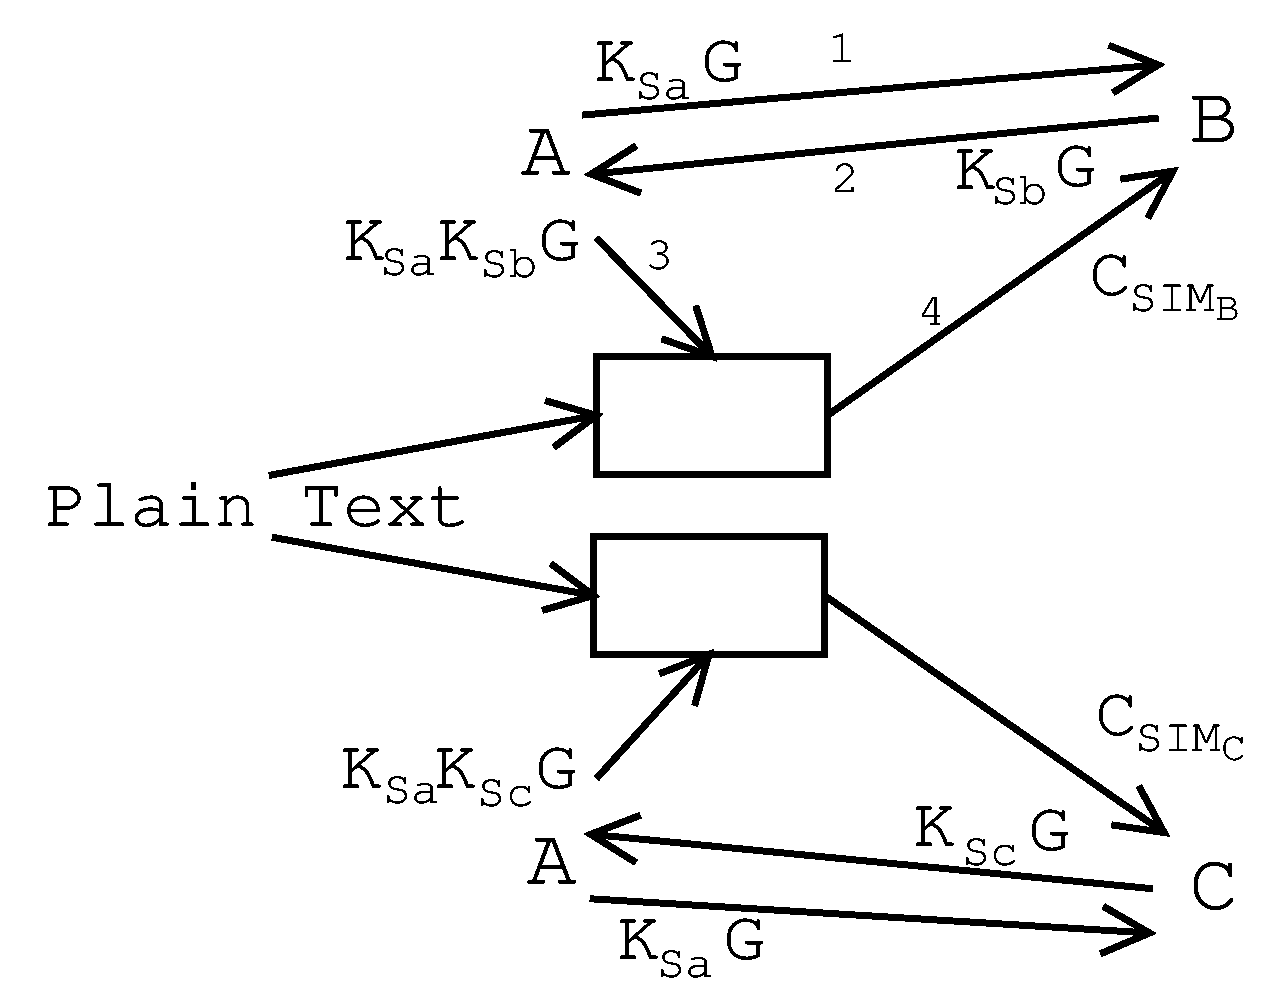
\includegraphics[scale=0.5]{./eps/DH.eps}
\end{center}
\caption{Scheme of a DH communication with two different receivers.}\label{DH.eps}
\end{figure}

\begin{figure}
\begin{center}
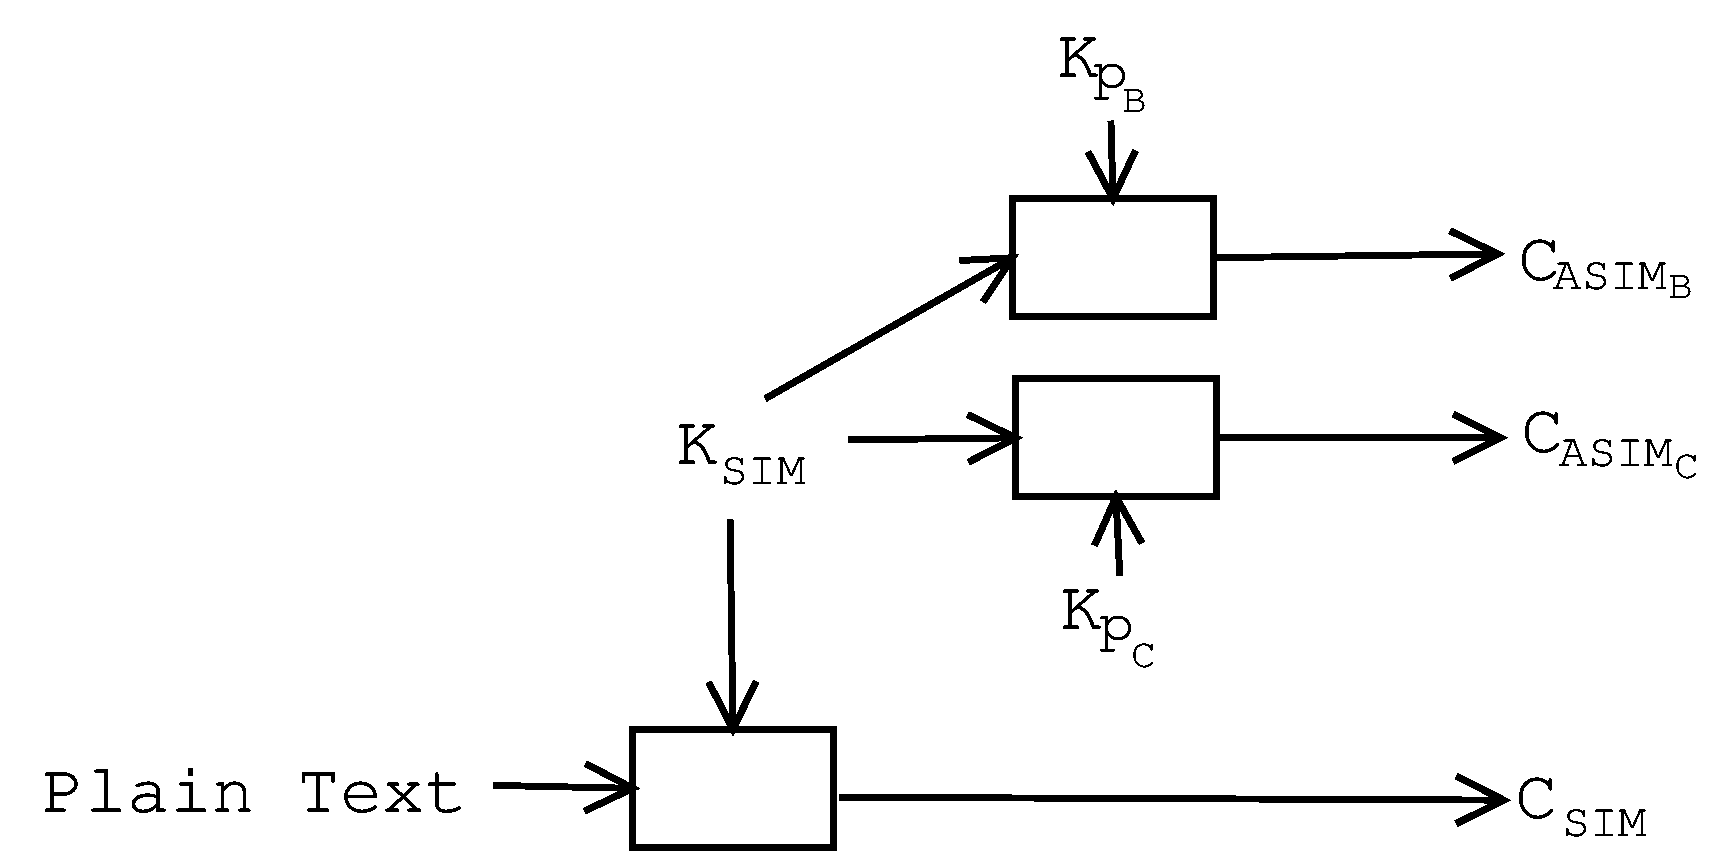
\includegraphics[scale=0.4]{./eps/ECElGamal.eps}
\end{center}
\caption{Scheme of a ECElGamal communication with two different receivers.}\label{ECElGamal.eps}
\end{figure}


In the offline schemes, as we need in mail communication, the cryptographic software makes a symmetric key and encrypt the plain text. Then the symmetric key are ciphered using public key schemes, and obtain $N$ little asymmetric cipher-texts. When the program makes the final cipher-text, it combines at the top a concatenation of all the little asymmetric cipher-texts, with the ciphered data with the symmetric scheme. At the decrypt time, the receiver search for the own identifier \footnote{It is not necessary to include the identifiers, in this case the program test all asymmetric cipher-texts and use the only one that it obtain a coherent symmetric key.} decrypt with its secret key to obtain the symmetric one, to finally recuperate the plain text.

In this case, the sent data is: $C_{ASIM_{B}} \cdot C_{ASIM_{C}} \cdot C_{SIM}$. There, $C_{ASIM_{B}}$ are probably a bit bigger than $K_{S_{b}}$, but $C_{SIM}$ is only sent one time and it has the same weight than \emph{plaint text}.

Without any standard scheme, we need to create or modify another one. The work that we did was to transform the classical ElGamal scheme over finite fields, over the new elliptic curve scheme. A deep study of the problem, and the searching of one intuitive solution of this scheme, we like to find really near to the classical ElGamal scheme:

\begin{algorithm}
\label{alg:ElGamal_cipher}
ElGamal encrypt scheme (with $\mathbb{F}_{p}^{*}$ group)
\end{algorithm}
\begin{enumerate}
\item Receive $input$
\item Generate k
\item $a=g^{k} \; \left( mod \; p \right)$
\item $b=y^{k} \; \left( mod \; p \right)$ /*$y=g^{x}$*/
\item $c=b\cdot input$
\item return $\left(a,c\right)$
\end{enumerate}

Attempt to find all the similarities between this schemes, we can obtain the next one:

\begin{algorithm}
\label{alg:ECElGamal_cipher}
ECElGamal encrypt scheme
\end{algorithm}
\begin{enumerate}
\item Receive $input$
\item Generate $k$
\item $R=k\cdot G$
\item $Q=k\cdot P$ /*$P=d\cdot G$*/
\item $c=Q_{x} \cdot input$
\item return $\left(R,c\right)$
\end{enumerate}

These two schemes are virtually the same, and we only need to append one rule because the public key size can be smaller than the symmetric one. This rule is not necessary in without curves schemes, because the relation between the key sizes are so hard. In the case of the elliptic curve scheme, it is an absurd thing but, we could use a bigger symmetric key (over 256 bits) that we encrypt with a public key over 192 bits; if we do not apply this rule, we loose the information at the encrypting time and we can not recuperate the original symmetric key to decrypt.

For this rule, we need to inform to the application in the other side of the communication about if the rule is used (without this the other side can not recuperate the information). For this reason we need to send a bit\footnote{The value of this bit is true if we apply the rule, or false if we do not need to use.} more of information.

To obtain the decrypt scheme, we proceed as the same way to translate the finite fields classical scheme over elliptic curves:

\begin{algorithm}
\label{alg:ElGamal_decipher}
Decrypt ElGamal scheme
\end{algorithm}
\begin{enumerate}
\item Receive $\left(a,c\right)$
\item $t_{1}= a^{x} \; \left( mod \; p \right)$ /*$\left(g^{k}\right)^{x}=\left(g^{x}\right)^{k}$*/
\item $t_{2}= t_{1}^{-1} \; \left( mod \; p \right)$
\item $output \; = c\cdot t_{2}$
\item return $\left(output\right) $
\end{enumerate}

\begin{algorithm}
\label{alg:ECElGamal_decipher}
Decrypt ECElGamal scheme
\end{algorithm}
\begin{enumerate}
\item Receive $\left(R,c\right)$
\item $Q=d\cdot R$ /*$d \left(k\cdot G\right)$*/
\item $Q'_{x}=Q_{x}^{-1}\; \left(mod \; p\right)$
\item $output \; = c\cdot Q'_{x}$ 
\item return $\left(output\right) $
\end{enumerate}

Virtually, we also obtained the same result, because the only change that we want to introduce is the inversion of the applied rule in the encrypting time.

\subsection{IFP ElGamal weakness.\footnote{Mikael Mylnikov report it.} \label{elgamalweak}}

In the section \ref{ECElGamal} is described the hybrid schemes drew in \ref{fig:hybrid}. Because of this, the plaintext that the asymmetric algorithm will encrypt has common properties. The smallest symmetric keys should not be less than 128 bits, until the common biggest schemes are over 256 bits.

The ElGamal scheme described in the algorithm \ref{alg:ElGamal_cipher} can be divided in two parts. The first part is related to the DLP or ECDLP and is the time to calculate the exponenciations, in a second time it is used one of the first part results to hide the plaintext. Break one of this parts are fatal. An effective attack is described in \cite{DJN}.

With the long keys used over $\mathbb{F}_p$ like 1024 bits or more, exist the problem and it is implemented an attack. But also are hard because factorize the cyphertext can be hard or the list of factors are too long. Over elliptic curves, the keys use less bits, between 192 and 521 if the curves are also defined over a finite field ($E\left(\mathbb{\mathbb{F}}_{p}\right)$).

\begin{figure}
\begin{center}
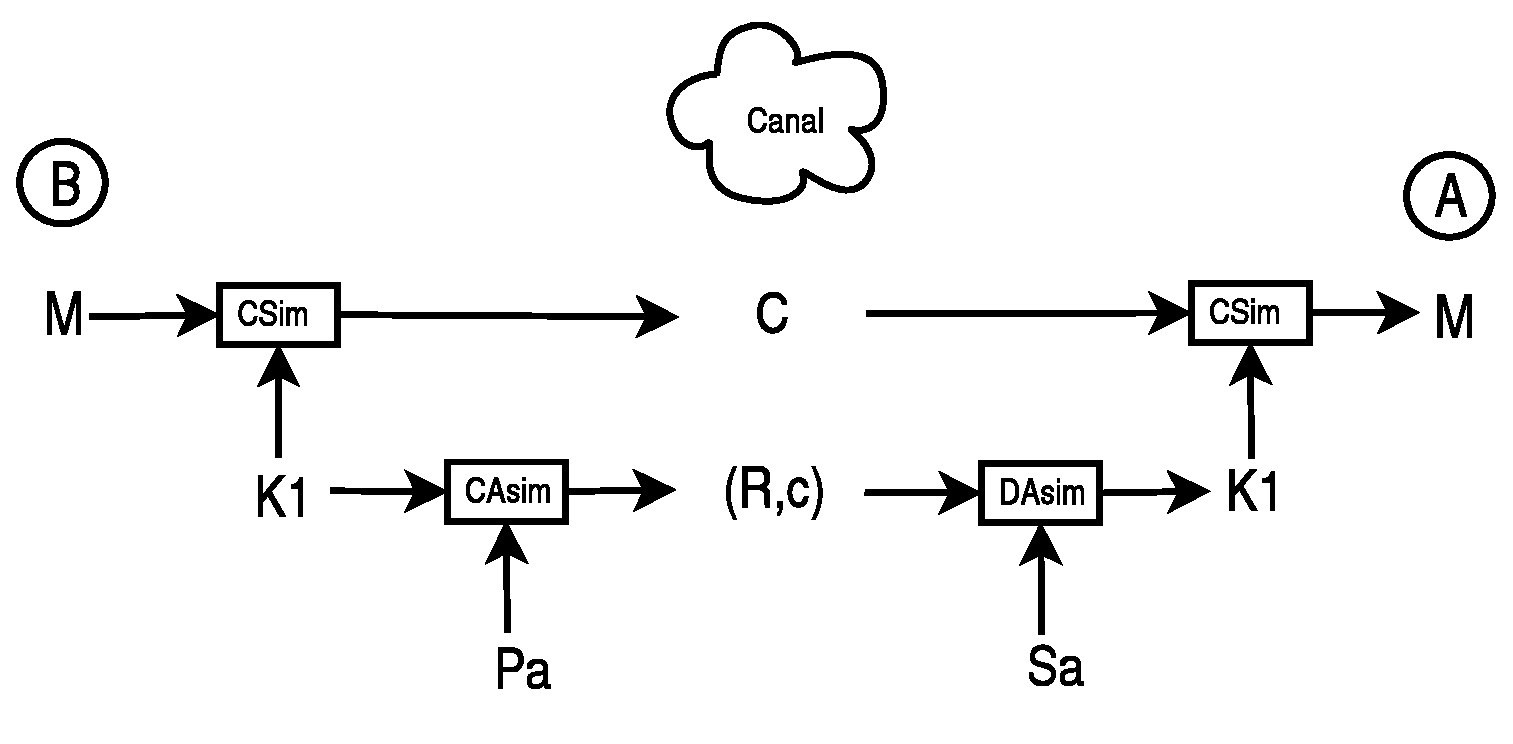
\includegraphics[width=10cm]{./eps/general.eps}
\end{center}
\caption{General scheme of an hybrid communication.}\label{fig:hybrid}
\end{figure}

The diagram \ref{fig:asym} describe the two parts division about we told before. To find the key to resolve the symmetric encryption it is needed to try to break the 'ecc' box or the 'x' box. Break the 'ecc' box is break the ECDLP and it is known that is a hard task, but not the same for the 'x' box. Factorize the value 'c' of at most 521 bits is possible. If the solution are to prime values, the solution are finded but the process is slow. If the factorization concludes with a long list of factors the process to find it is so fast.

With this list of factors, will rest a process to combine it  

\begin{figure}
\begin{center}
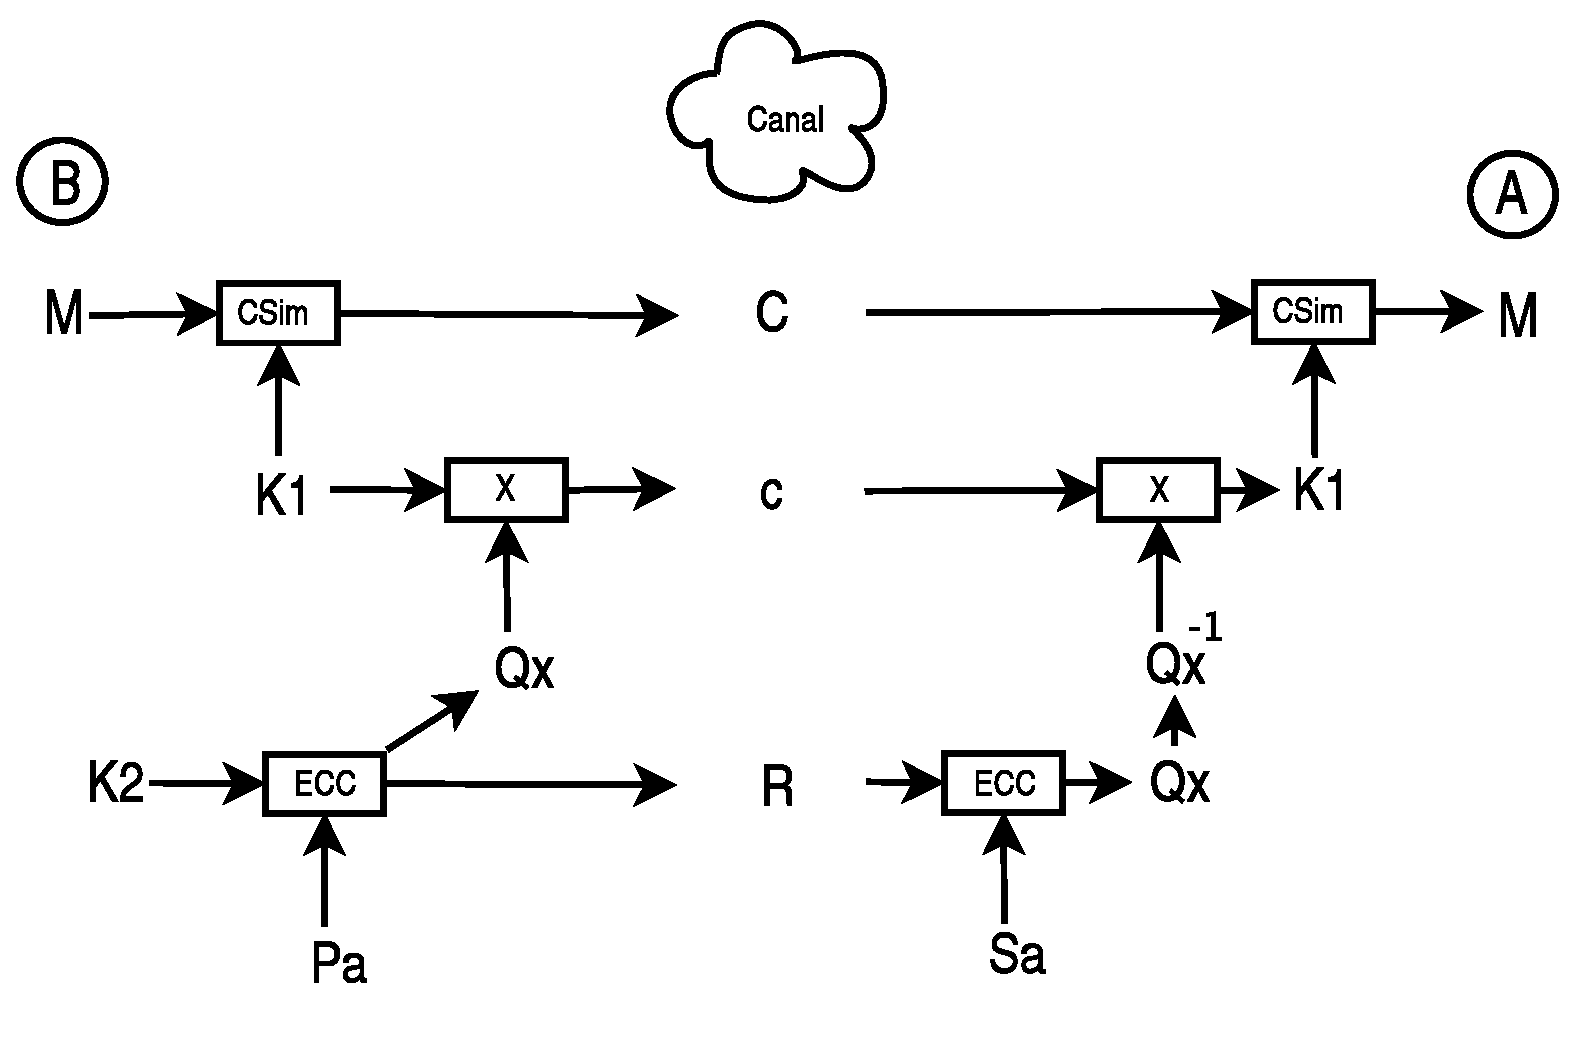
\includegraphics[width=10cm]{./eps/ecc.eps}
\end{center}
\caption{Hybrid scheme with a detail of the asymmetric.}\label{fig:asym}
\end{figure}

\begin{figure}
\begin{center}
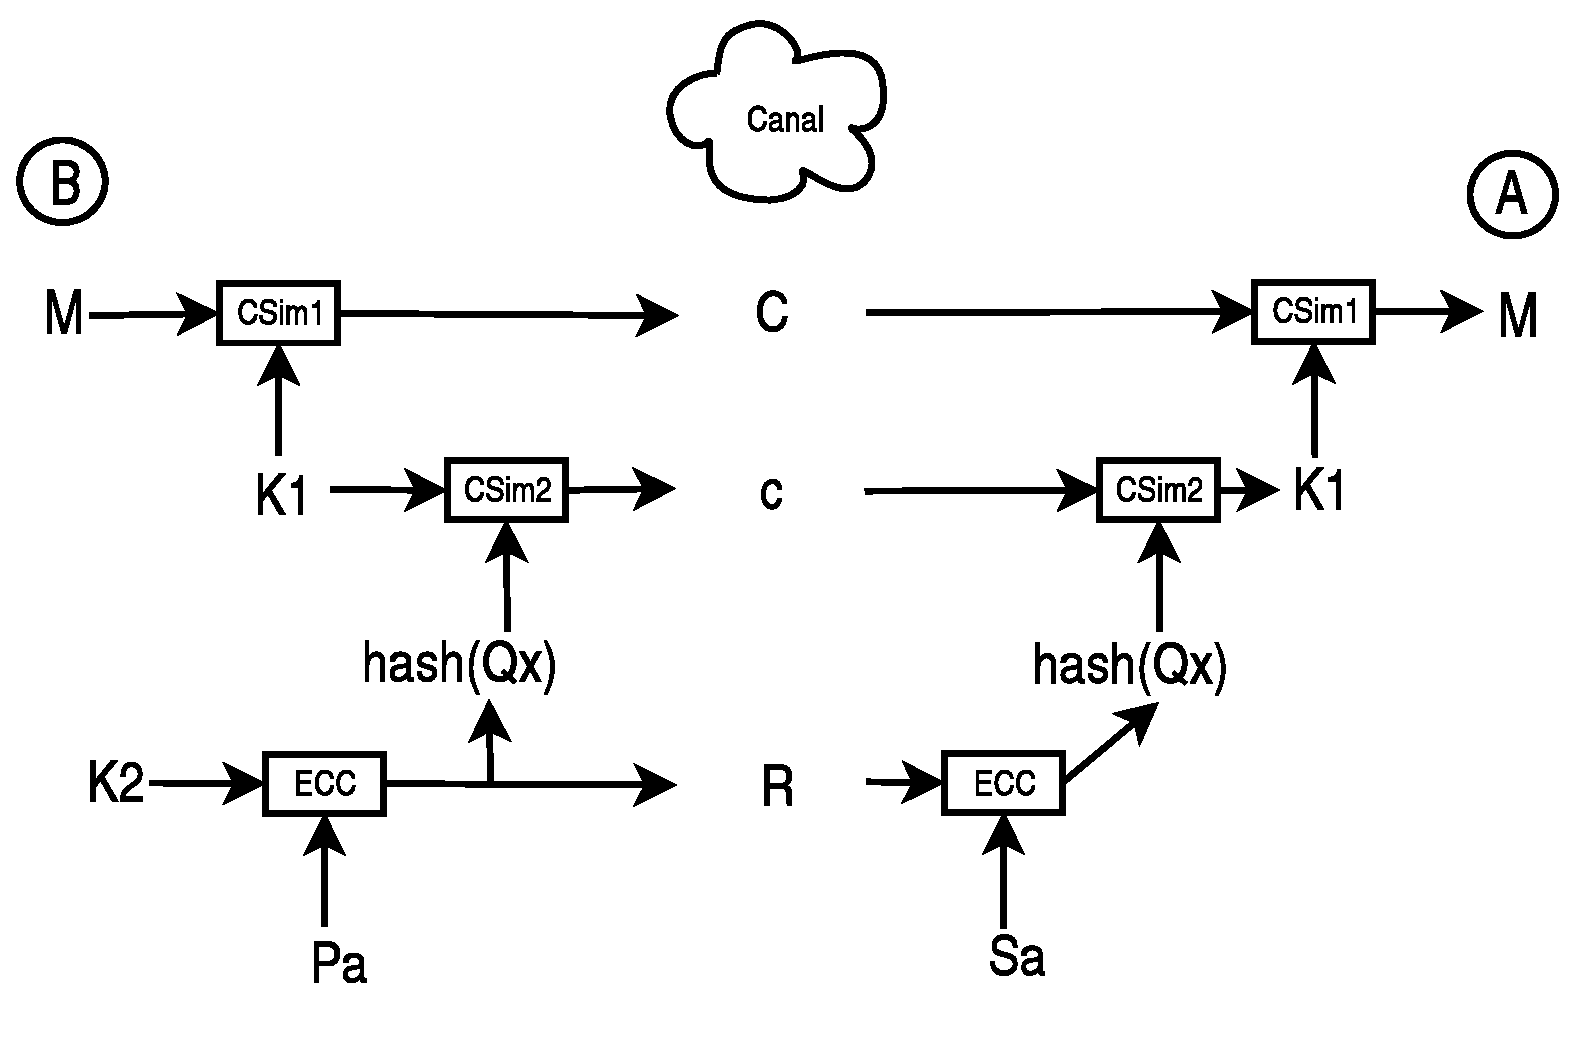
\includegraphics[width=10cm]{./eps/ecc.mod.eps}
\end{center}
\caption{Proposal to solve the IFP ElGamal weakness.}\label{fig:dhaes}
\end{figure}

\section{ECDSA \label{ECDSA} }

In the same way to which we obtain a new scheme virtually equivalent over points on a curve based on the classical finite field scheme, we can find to the digital signature a DSA scheme connected to the elliptic curve over the ECDSA name. But now, we do not need to do this, because this scheme is part of the rule \cite{P1363} of the IEEE institution. About this signature scheme, we could see the algorithm \ref{alg:Firma}; and the same in the verification that it is in the algorithm \ref{alg:Verificacio-firma}.

The sign and verification schemes obtained in the rule of the IEEE keep the NIST standard described in \cite{NIST}. Thanks of this keep an international acknowledged standard, we can say the own algorithmic and the code are ok to the use, and moreover it adapt to all the softwares that other people can implement. The NIST standard that we explain, do not say what do you do to make an elliptic curve digital signature scheme, else it explain about the things that the  algorithm need to complain, and after the code, that they lake to follow the DSS standard, about digital signature.

Anyway, and without resting importance to this point, the main use of the NIST standard is in the Appendix 6. In this appendix we have a detailed recommendation about what need to complain all the elliptic curve schemes for a governmental use (it understand in the United States, that is the influence zone for this standard).

\chapter{GnuPG}

Gnu Privacy Guard is a complete and free\footnote{free in the direction of this is a open source program} program based in the standard OpenPGP. This program has the same quality to the popular program Pretty Good Privacy (PGP is originally developed by Philip Zimmermann el 1990), with one advantage: the present program does not use any patented algorithm (IDEA for example), and this can be used without restrictions. This software is based and we can consider it as a programming language translation of the RFC \cite{rfc2440}. Its version 1.0.0 was liberated in September of 1999 and now we have available the version 1.2.3, but in this project we work with the version 1.2.1. GnuPG is an Open Source Software, and we can use it 'without restrictions'. You can use it freely, modify it, and distribute it, always over the terms of the Gnu General Public License (further on GLP).

GnuPG is a good tool for the secure communication and secure storing of data, and we can use it for encrypt data or for the digital signature of this data. The present stable version is named 1.2.x, big or deep modifications do not exist in these versions; the developers only pretend to polish bugs and fix compatibilities. In the versions 1.3.x we use to developing and contain the new tools that they pretend to append in the next stable branch 1.4.x in a non far future. Finally, there is another developing branch named 1.9.x. this is an experimental branch to join the \textit{Aegypten} project with the \textit{gpg-agent} project, the daemon for \textit{smart-card}, and the gpg for S/MINE. For the requirements of multiple platform support, the POSIX compatibility has an immense importance. The code of the 1.9.x branch are based on the code of the actual developers version 1.3.

\section{Program structure \label{sec:estruc} }

The program structure is not complicated. The code is delivered in multiples directories, according to the content code. Evidently, there is a root directory, in which we can find information about the program and the program environment. Especially we need to know that where the '\textit{configure}' and '\textit{Makefile}' files are, and we need to pay attention to the '\textit{configure.ac}' and '\textit{Makefile.in}' files, but we are going to see it more deeply in section \ref{sec:Autotools}.

The main directories we can have anxiety to see, can be put in order depending on the contained importance. The paramount to consult is the '\textit{./doc/}' directory; there we can find the document after that are placed in the Unix manual accessible with '\textit{\$ man gpg}', and we can find a describing file named '\textit{./doc/HACKING}'. It is in this last file where we obtain one guide to visit the program structure and the source code. If anybody makes a modification in the program structure, it is in this file the place they need to reflect its change, and for as will be easy to localize.

\begin{center}
\begin{tabular}{ll}
Directory Layout & ~
\tabularnewline
\hline
  ./		& Readme, configure
\tabularnewline
  ./scripts	& Scripts needed by configure and others
\tabularnewline
  ./doc 	& Documentation
\tabularnewline
  ./util	& General purpose utility function
\tabularnewline
  ./mpi 	& Multi precision integer library
\tabularnewline
  ./cipher	& Cryptographic functions
\tabularnewline
  ./g10 	& GnuPG application
\tabularnewline
  ./tools	& Some helper and demo programs
\tabularnewline
  ./keybox	& The keybox library (under construction)
\tabularnewline
  ./gcrypt	& Stuff needed to build libgcrypt (under construction)
\tabularnewline
\hline
\end{tabular}
From '\textit{./doc/HACKING}'.
\end{center}


The other important directories we like to visit are '\textit{./cipher/}', '\textit{./mpi/}', and '\textit{./g10/}'. In the fist one, '\textit{./cipher/}', the name shows that it contains all the encrypt and decrypt modules. But not only there are the asymmetric key modules, but  also there are the symmetric key modules. The other type of modules this directory contains are the digital signature modules, the directory name does not indicate it, but it is evident that modules can not reside in another place. As the same, there are resume functions to obtain the hash of the data that we will like to sign.

We need to pay an especially attention to some files of this directory '\textit{./cipher/}'. The main one which we are interested in is: '\textit{./cipher/pubkey.c}'; in this file there is the data structure that enumerated all the public key algorithms (or isometrics) that the program supports to use. If we does not include the own module in this table, the program do not recognize it, no matter how much the code was included in the compilation. We can observe that the other modules are also in the table, and in the beginning of this are included the header files of that. Then we need to append the information in the table and the '\#include ``ecc.h''' in the beginning.

Other important files, in spite of we do not describe it (because it will be described in the section \ref{sec:Autotools}, or because the file does not have a direct relation with the own module) are '\textit{./cipher/cipher.c}' and '\textit{./cipher/algorithms.h}'. This files have the same objective than the last one, but for the symmetric and hash algorithms, respectively.

In the own module programming task, we need to arrange basic mathematical operations, because we do not use a conventional data structures, but we need arithmetical functions for big numbers and we need to represent it in special structures. This software facilities it, in a mathematical library named '\textit{Libgcrypt}'', but there only included the section to the big integers and this library is named '\textit{Multi-Precision Integers}' (further on MPI).

Once we have this information, we can suppose that this directory is saved the mathematical library in the program: '\textit{./mpi/}'. The only thing that we need to comment about this library, is the existence of the proper subdirectories with the assembler code to the different architectures, because of the efficiency motives the low-level operations are made in this language (evidently, there is one generic implementation, for the non contemplated architectures).

Before going to see the main directory ('\textit{./g10/}'), we need the visit another one that it has not importance for the contained code, but the importance resides in the general level of the program. This directory is '\textit{./include/}'. About the contained files, there are four interesting files, but two of them are really important. The main one to the own intention is: '\textit{./include/cipher.h}'. In this there are the list of all the encryption algorithm that this software supports, add more with this identifier number assigned in the RFC \cite{rfc2440} in the section about constants (p, p.49). The next important file to see is '\textit{./include/mpi.h}', because in this  we can find a complete list of the primitives that we can use over the big number mathematical library. Finally, the other two files with an importance to see are '\textit{./include/util.h}' and '\textit{./include/types.h}'. In the first one we use in the debugging time, because it contain the name of functions how call to show information in the execution time. While in the second file, the data structure proper of the program is identified.. There are different data structures thought to avoid problems with the size of an unsigned integer dependent on the architecture (16, 32, 64 bits).

Now we are going to see the main directory in the program: '\textit{./g10/}'. In this directory, there are only two interesting files for us, but  these files are the most necessary files to see the results of the own work. We need to modify more files to the correct performance of the program, but this is because of the interface module-program. The first important file, and probably the most important one, is '\textit{./g10/keygen.c}', what this file contains are the tasks to do when we execute the program to generate a new key with the command '\textit{\$ ./gpg --gen-key}'. The modifications did where it to allow the access to the own module with the intention create a new elliptic curve key. The other important file is: '\textit{./g10/g10.c}', we can imagine, because the file name, that this is the main file of the program. It is in this one where are made the decision to go to another one to realize the requested task in the command line is made. Finally, the other changed files are: '\textit{./g10/getkey.c}', '\textit{./g10/keyid.c}', and '\textit{./g10/misc.c}'.

\subsection{Autotools \label{sec:Autotools} }

~\\In the way to create an executable file with all the codes, and given that there are a lot of source files, we can see that to create manually a \textit{Makefile} is a titanic work. To do this, there exist Gnu tools for the applications development that automatize this task. We talk about the Autotools. This development tool provides the needed and really useful \textit{scripts} files to generate the configuration files and process the compilation option. The use of this tools permits to concentrate ourselves in the code, and less the load to think of the subtle differences between different UNIX\footnote{We can not forget that with this standard programming we can compile over Windows and MacOS platforms, and in this platforms the differences are bigger.}.

The first tool to use offered in Autotools is the \textit{autoconf}. This one produces the script who prepare the code to adapt itself to the present system. The result of these tools is the shell script '\textit{./configure}', to prepare the compilation. The results also we can see in the named file '\textit{config.h}', that contain the preprocessor macros that it will need depending on the platform. The task of the '\textit{./configure}' script is to comprovate the portability to the present platform that we want to install, depending on the necessities of the '\textit{Makefile}s', header files, and other specific. The installer user does not need to modify any file manually.

The second tool to make easy the compilation is the \textit{automake}. When the installer wants to use the results of this tool, the code was prepared to the present platform. The task that we need to do now is the compilation and linking of the source and the object files. The tools to do this, generate all the necessary \textit{Makefile}. With the \textit{automake} tool is generated the '\textit{Makefile.in}' (that the \textit{./configure}' script need to create '\textit{Makefile}') from the specification written in the '\textit{Makefile.am}'. We need to remember, there are three different '\textit{Makefile*}'. The result of the Autotools application agrees with the GNU standards, and the tool \textit{autoconf} is always necessary for the appropriate use.

\begin{figure}
\begin{center}
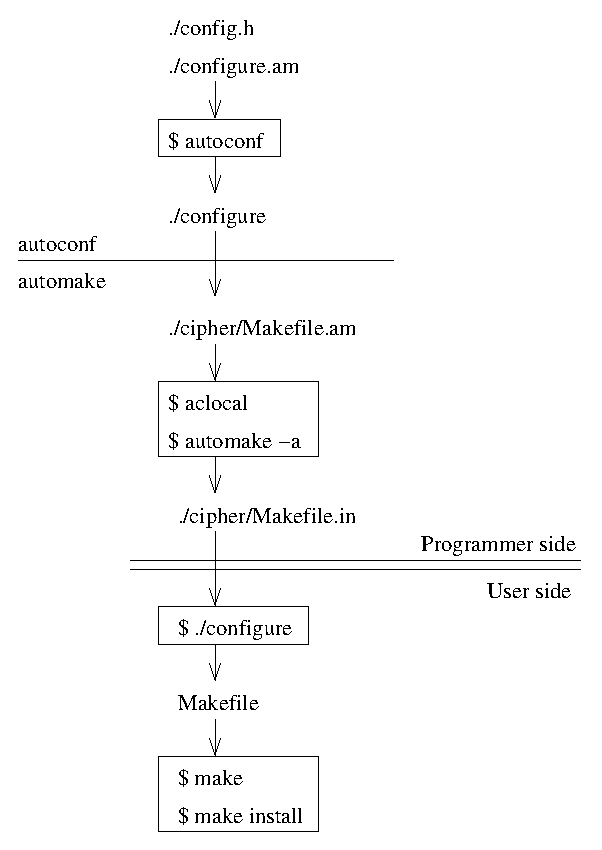
\includegraphics{./eps/autotools.eps}
\end{center}
\caption{Autotools Scheme.}
\end{figure}

There exist a third tool in the Autotools pack named \textit{libtool}. In which i will make an appointment only because it is not used in this program. This tool is used to generate the shared libraries, and not to require neither \textit{autoconf} nor \textit{automake}, but sometimes it interact with themselves.

The main virtues of the Autotools are two. The first one, is the work due to simplifies the portability code in the '\textit{./configure}' file; and the second virtue is to simplifies the compilation in applications with a distributed sources, compiling it in a recursive procedure.

Probably all the big application needs the offered help of the \textit{autotools} which are structured in different subdirectories. We saw in the section \ref{sec:estruc} that own program is not an exception and maintains different directories depending to the source destination. Because of this, we can not have only one \textit{Makefile} we have one per directory and the compilation will due in a recursive form. So, the new module insertion does not affect the \textit{./configure} script, because it prepares the system without importance in the number of modules that have the application.

The \textit{Makefile} that we need to introduce the changes to the code insertion is hosted in: '\textit{./cipher/Makefile.am}'. If we edit it, we can see a list of the sources hosted in this directory, and the work that it  only needs to do is to insert the module name to this list. This list is labeled with the variable '\textit{libcipher\_a\_SOURCES}'. This file is not long, it follows a pattern and almost contains the source list.

When we append the name of the own module to the list, we can use the autotools. Because the modification is in the '\textit{./cipher/Makefile.am}' file, and we do not touch anything of the '\textit{./configure.in}' file\footnote{In fact, the distribution do not contain this '\textit{./configure.in}' file else contain the '\textit{./configure.ac}' we can not execute '\textit{\$ autoconf}' without the first.} we do not need to execute '\textit{\$ autoconf}', and we can go directly to execute '\textit{\$ aclocal}' and '\textit{\$ automake -a}'. Because the distribution was created, all the needed files are existing.

The autotools are applied, we have all the needed things to make the new distribution. We can execute '\textit{\$ ./configure}' to start the program installation.

\section{ECC Module}

We can start the work and talk about the algorithms and the implemented code. Basically, the work is due to two phases. The first one is to collect and create the needed algorithms for all the operations to realize, and the second task is to translate these algorithmics to a higher level programming language.

Starting with the algorithmics, we can distinguish five different types depending on the task that they realize. In a first level we can separate three types: key pair generation algorithms, encrypt/decrypt algorithms, and the digital sign/verification algorithms. In a second level, below the last one we can put the auxiliary algorithms to the up-layer. We can divide this level in two types of algorithms: the key pair generation auxiliary, and the algorithms that they do the closed operations between points of the elliptic curve. This second type, can be considered in a third descending level , because it is used for the algorithms of the all other types, as much in the first group as in the second one.

In the implementation way, we use the high level language '\textbf{C}' for two reasons. The first one is the used language n the GnuPG program, because the whole of it is written in this language, and the second reason is the council given by \textit{Robert J. Hansen} in the way of the target audience that can hack this code.

The functions, at the same time, and they come from the algorithmics translation, can be divided it in groups. But we make a different division to the implementation division. The first division difference is between mathematical functions and the cryptographycal functions. And because we have a big numbers library in the program, also we make references to the functions that we need in the programming (evidently we do this in the mathematical functions section).

\subsection{Needed algorithmics}

~\\Here we relate in detail all the algorithms that later we will implement. There was someone's algorithm that it was extracted form the IEEE standard: \cite{P1363}, while other algorithms that they are not present in any standard, they are written here at the first time. Without more preambles we can go to see this.

\subsubsection{EC Key Generation \label{genkey}}

~\\The first thing that we will do to put on the new public key cryptosystem is to generate a key pair. To generate it, first of all we will decide in which parameters the cryptosystem works, the same as: all the values that it needs to start:

\begin{algorithm}
\label{alg:Generar-setup}Setup Generation.

Input: Prime of big order '$p$'($ord\left(p\right)$). /{*}$\left\Vert p\right\Vert \in\left\{ 192,224,256,384,521\right\} ${*}/

Output: Parameters of the elliptic curve ($E\left(\mathbb{\mathbb{F}}_{p}\right)$)./{*}$p$ ($\mathbb{F}_{p}$);$a$,$b$ ($E\left(a,b\right)$);$n$,$h=1$ (ord(G),cofactor);$G${*}/
\end{algorithm}
\begin{enumerate}
\item Select the curve $E\left(\mathbb{\mathbb{F}}_{p}\right)$ over a  $\mathbb{F}_{p}$ in the way $p_{min}\leq p\leq p_{max}$.
\item Fixate the values $p$,$a$,$b$,$n$.
\item Search the generator $G$ of the cyclic subgroup according to \ref{alg:Obtenir-generador}.
\item Return $p$,$a$,$b$,$n$ and $G$.
\end{enumerate}
~

At the time the setup is generated, we can create a new private key, and after that the public key:

\begin{algorithm}
\label{alg:Generar-parell}Generate key pair (\texttt{\small p1363-A.16.9})

Input: Parameters $p$, $a$, $b$, $n$, and $h$ of one elliptic curve ($E\left(\mathbb{F}_{p}\right)$), and the generator point $G\in E\left(\mathbb{F}_{p}\right)$.

Output: Public key $P$, and secret key $d$.
\end{algorithm}
\begin{enumerate}
\item Generate an integer $d$ in the range $0<d<n$.
\item Calculate $P=d\cdot G$.
\item Return $d$ and $P$.
\end{enumerate}
~

Due to possible mistakes (and why not attacks), we need to verify if the received key is ok or on the contrary its key suffers some disturbances (or malicious modifications):

\begin{algorithm}
\label{alg:Verificacio-clau}Key verification

Input: An elliptic curve ($E\left(\mathbb{F}_{p}\right)$), and the public key $P$.

Output: Boolean value of acceptation or rejection
\end{algorithm}
\begin{enumerate}
\item Comprovate $P\neq\mathcal{O}_{E}$.
\item Comprovate $n\cdot P= \mathcal{O}_{E}$.
\item Return 'true' if all comprovation are ok, in other case 'false'.
\end{enumerate}
~

\subsubsection{EC auxiliary functions to the Key Generation. \label{genkey_aux} }

~\\To realize the operation of the \ref{genkey} section, we need the subfunctions in one descendant level. And now we start to explain it.

The first that we need is called the algorithm \ref{alg:Generar-setup}. This algorithm at the same time reposes over another one that later we will be able to see.

\begin{algorithm}
\label{alg:Obtenir-generador}Obtain a generator point with a big prime order (\texttt{\small p1363-A.11.3})

Input: A big prime ($n$), an positive integer non divisible by n ($h$ such than $n\nmid h$), an elliptic curve ($E\left(\mathbb{F}_{p}\right)$)

Output: If \#$E\left(\mathbb{F}_{p}\right)=h\cdot n$, return the point $R\in$$E\left(\mathbb{F}_{p}\right)$ with the order $n$. Else, error.
\end{algorithm}
\begin{enumerate}
\item Generate a random point $P\neq\mathcal{O}_{E}$.
\item $R\leftarrow h\cdot P$.
\item If ($R=\mathcal{O}_{E}$)\{goto 1\}.
\item $Q\leftarrow n\cdot R$.
\item If ($Q\neq\mathcal{O}_{E}$)\{error\}./{*}invalid order{*}/
\item Return $R$.
\end{enumerate}
~

It is not difficult to generate a random point in an elliptic curve, we only need to find one integer that it can generate a valid coordinate of the curve. Exactly, our knowledge about if the value can proportionate one valid coordinate, or nor, depends on if we can calculate a square root.

\begin{algorithm}
\label{alg:random-punt}Find a random point in the elliptic curve
(\texttt{\small p1363-A.11.1})

Input: A prime integer ($p>3$), the parameters from the elliptic curve($a,b\in\mathbb{F}_{p}\mid E\left(\mathbb{F}_{p}\right)=\left(y^{2}=x^{3}+ax+b\right)$)

Output: A random point over the curve ($P\neq\mathcal{O}_{E},P\in E\left(\mathbb{F}_{p}\right)$)
\end{algorithm}
\begin{enumerate}
\item Generate a random $x$ such that $0\leq x<p$.
\item $\alpha\leftarrow x^{3}+ax+b$ $\left(mod\; p\right)$.
\item If ($\alpha=0$)\{Return $P=\left(x:0:1\right)$\}.
\item If (!$\exists\left(\beta\leftarrow\sqrt{\alpha}\right)$)\{goto 1\}.
/{*}$\beta^{2}\equiv\alpha$ $\left(mod\; p\right)${*}/
\item Generate random bit $\mu$.
\item $y\leftarrow\left(-1\right)^{\mu}\beta\:\left(mod\; p\right)$.
\item Return $P=\left(x:y:1\right)$.
\end{enumerate}
~

The work of finding the square root of a big integer in a finite field is not an easy task. What makes this work especially complicated, is that can not know if this value exists or not into the finite field. To comprovate if this value exist we could calculate a sequence of numbers named \textit{Lucas values}.

\begin{algorithm}
\label{alg:square-root}Find, if it exist, the square root of one number module a big prime. 
(\texttt{\small p1363-A.2.5})

Input: A big prime ($p$), an integer ($g\mid0<g<p$)

Output: If exist:$z=\left(\sqrt{g}\right)\left(mod\; p\right)$, else -1 ($NULL$).
\end{algorithm}
\begin{enumerate}
\item If ($p\equiv3\;\left(mod\:4\right)$)\{/{*}such that $p=4k+3${*}/

\begin{enumerate}
\item $z=g^{k+1}\;\left(mod\: p\right)$\}
\end{enumerate}
\item if ($p\equiv5\;\left(mod\:8\right)$)\{/{*}such that $p=8k+5${*}/

\begin{enumerate}
\item $\gamma=\left(2g\right)^{k}\;\left(mod\: p\right)$
\item $i=2g\left(\gamma^{2}\right)\;\left(mod\: p\right)$
\item $z=g\gamma\left(i-1\right)\;\left(mod\: p\right)$
\end{enumerate}
\item If ($p\equiv1\;\left(mod\:8\right)$)\{/{*}such that $p=8k+1${*}/

\begin{enumerate}
\item Generate a random $p'$ such that $0\leq p'<p$.
\item Search the Lucas sequence values

\begin{enumerate}
\item $V=V_{\frac{p+1}{2}}\;\left(mod\: p\right)$ i 
\item $Q_{0}=Q^{\frac{p-1}{4}}\;\left(mod\: p\right)$
\end{enumerate}
\item $z=\frac{V}{2}\;\left(mod\: p\right)$
\item If ($z^{2}\;\left(mod\: p\right)=g$)

\begin{enumerate}
\item Return $z$.
\end{enumerate}
\item If ($Q_{0}>1$ \&\& $Q_{0}<\left(p-1\right)$)

\begin{enumerate}
\item Return $-1$.
\end{enumerate}
\item else, goto 3.a.
\end{enumerate}
\end{enumerate}
~

\begin{definition}
The formal definition of the Lucas Sequence is:\\
\begin{center}
$V_{0}=2;\; V_{1}=p;$
\end{center}
\begin{equation}
V_{k}= \left( p \cdot V_{k-1} \right) - \left( q \cdot V_{k-2} \right) \; for k \geq 2
\end{equation}
\end{definition}

%%<!--
%%    Com explicar algo que no entenc?
%%//-->

\begin{algorithm}
\label{alg:Lucas}Generate Lucas sequence values (\texttt{\small p1363-A.2.4})

Input: A prime ($n$), two integers ($p'$ and $q'$), a positive integer ($k$)

Output: $V_{n}\;\left(mod\: n\right)$ and $Q_{o}^{\left\lfloor k/2\right\rfloor }\;\left(mod\: n\right)$
\end{algorithm}
\begin{enumerate}
\item Initialize: $v_{0}=2$; $v_{1}=p'$;$q_{0}=1$; $q_{1}=1$;
\item $k=k_{r}k_{r-1}\ldots k_{1}k_{0}$/{*}$k_{r}=1${*}/
\item From $i=r$, to $i=0$, down $--1$\{

\begin{enumerate}
\item $q_{0}=q_{0}\cdot q_{1}\;\left(mod\: n\right)$
\item If ($k_{i}=1$)\{

\begin{enumerate}
\item $q_{1}=q_{0}\cdot q'\;\left(mod\: n\right)$
\item $v_{0}=v_{0}\cdot v_{1}-p'\cdot q_{0}\;\left(mod\: n\right)$/{*}$t1=v_{0}\cdot v_{1}$ ; $t2=p'\cdot q_{0}${*}/
\item $v_{1}=v_{1}^{2}-2\cdot q_{1}\;\left(mod\: n\right)$\} /{*} $t1=v_{1}^{2}$ ; $t2=2\cdot q_{1}${*}/
\end{enumerate}
\item Else\{

\begin{enumerate}
\item $q_{1}=q_{0}$
\item $v_{1}=v_{0}\cdot v_{1}-p'\cdot q_{0}\;\left(mod\: n\right)$/{*}$t1=v_{0}\cdot v_{1}$ ; $t2=p'\cdot q_{0}${*}/
\item $v_{0}=v_{0}^{2}-2\cdot q_{0}\;\left(mod\: n\right)$\} /{*} $t1=v_{0}^{2}$ ; $t2=2\cdot q_{0}${*}/
\end{enumerate}
\end{enumerate}
\item return ($v_{0}$, $q_{0}$)
\end{enumerate}
~

At this point, in the algorithmic view, we can have the key pair of the own cryptosystem. We can start to use it.

\subsubsection{ECElGamal}

~\\We saw how we could obtain the encrypt algorithms in the section \ref{ECElGamal}, and now explanations are not necessary. It is exactly equal than the last algorithms, but they are equivalent.

\begin{algorithm}
\label{alg:Xifrat}Encrypt ($A\rightarrow B$). (\texttt{\small p1363-7.2.1})

Input: Public key ($pkey_{B}$) and numeric plain text ($z$).

Output: Resultant point ($R$), cipher ($c$).%, bit indicator of the stile of $z'$ ($bit$).
\end{algorithm}
\begin{enumerate}
\item Generate key session ($k$)
%\item If (size($z$) > size($pkey_{B}.n$))\{

%\begin{enumerate}
%\item $z'=z-pkey_{B}.n$;
%\item $bit=1$;\}
%\end{enumerate}
%\item Else\{$z'=z$;$bit=0$;\}
\item $P=k\cdot pkey_{B}.Q$ /{*}$Q_{B}=d_{B}\cdot G_{B}$;$P=k\cdot d_{B}\cdot G_{B}${*}/
\item $R=k\cdot pkey_{B}.G$
\item $c=z'\cdot P_{x}$
% \item If (size($c$)<size($pkey_{B}.n$))\{jump to 1;\}
\item Return ($R$,$c$);%,$bit$);
\end{enumerate}
~

\begin{algorithm}
\label{alg:Desxifrat.}Decrypt. (\texttt{\small p1363-7.2.1}) %/{*}!! '$n$' o '$p$' !!{*}/

Input: Resultant point ($R$), cipher ($c$), and private key ($skey_{B}$)

Output: numeric plain text ($z$)
\end{algorithm}
\begin{enumerate}
\item Received ($R$,$c$)%,$bit$)
\item $P=skey_{B}.d\cdot R$ /{*}$P=d_{B}\cdot k\cdot G_{B}${*}/
\item $z=c\cdot P_{x}^{-1}\:\left(mod\; p\right)$.
%\item If ( $bit=1$)\{

%\begin{enumerate}
%\item $z=z'+pkey_{B}.n$;\}
%\end{enumerate}
%\item Else\{$z=z'$;\}
\item Return ($z$);
\end{enumerate}
~

\subsubsection{ECDSA}

~\\In the section \ref{ECDSA} we make reference to the next description algorithms. These schemes are virtually the same than the schemes that we can find without the Elliptic Curve Cryptosystems, the difference is in the operation realized with the public key due to this case is not a number, it is a point (After the operation, we extract the coordinate $x$).

\begin{algorithm}
\label{alg:Firma}Sign ($A\rightarrow B$) (\texttt{\small p1363-7.2.7})

Input: Public key ($skey_{A}$) and message hash (\#hash).

Output: Number pair $\left(r,s\right)$/{*}such that $0<r,s<skey_{A}.n${*}/.
\end{algorithm}
\begin{enumerate}
\item Generate session key '$k$'.
\item $I\leftarrow$$k\cdot\left(skey_{A}.G\right)$.
\item $i\leftarrow I_{x}$.
\item $r\leftarrow i\left(mod\: skey_{A}.n\right)$.
\item If $r=0$: goto 1.
\item $s\leftarrow k^{-1}\cdot\left(\# hash+\left(skey_{A}.d\right)\cdot r\right)\left(mod\: skey_{A}.n\right)$
\item If $s=0$: goto 1.
\item Return $\left(r,s\right)$.
\end{enumerate}
~

In the verification sign, we can see all the operations that we can realize with an elliptic curve point. As the same that in the signature procedure, it needs to calculate the scalar multiplication of a point (two times in this case); but here it needs more and add two points.

\begin{algorithm}
\label{alg:Verificacio-firma}Sign verification (\texttt{\small p1363-7.2.8})

Input: Public key ($pkey_{A}$), message hash (\#hash), and number pair $\left(r,s\right)$.

Output: Boolean value of acceptation or rejection.
\end{algorithm}
\begin{enumerate}
\item Verifies $\left(r,s\right)\in\left[1,\left(pkey_{A}.n\right)-1\right]$.
\item $h\leftarrow s^{-1}\left(mod\: pkey_{A}.n\right)$.
\item $h_{1}\leftarrow\left(\# hash\right)\cdot h\left(mod\: pkey_{A}.n\right)$.
\item $h_{2}\leftarrow r\cdot h\left(mod\: pkey_{A}.n\right)$.
\item $Q\leftarrow h_{1}\cdot\left(pkey_{A}.G\right)+h_{2}\cdot\left(pkey_{A}.P\right)$.
\item If $Q=\mathcal{O}_{E}$: refuse.
\item $i=Q_{x}\left(mod\: pkey_{A}.n\right)$.
\item If $i=r$ accept; else: refuse.
\end{enumerate}
~

There are references made to operations in a lower level in all the algorithms. We describe someone, for example the low operation over the field definition, but there are other algorithms that they need, that will be for the times that it is called, or for the possibility of improvement the efficiency and speed up of this.

\subsubsection{Closed operation between Elliptic Curve Points (over $\mathbb{F}_{p}$, with projective coordinates) \label{ops_tancades} }

~\\In this section there are also made in a descent way to make an easy compression, and remark the importance. The first question that you make about one point that you have is if this is Point at infinity, or not. We need to remark, but in what we are interested in is to know is if this is a Point at infinity of the elliptic curve that we use (denoted for $\mathcal{O}_{E}$), in the case that this point is another Point at infinity (in general, the Point at infinity is denoted for $\mathcal{O}$) or if this is an invalid point out of the curve we receive an error. In spite of this aclaration, the function suppose that the point of the input is a valid elliptic curve point.

\begin{algorithm}
\label{alg:Bool-P-infinit}Point at infinity of the curve: $\mathcal{O}_{E}$

Input: Valid point of the curve ($Q$).

Output: Error, If this is not a valid curve point; True, If this is a Point at infinity of the curve (no include all the $\mathcal{O}$ of the projective plan); False, in other case.
\end{algorithm}
\begin{enumerate}
\item If ($Q_{z}=0$)\{

\begin{enumerate}
\item If ($Q_{y}=0$)\{Return (error);\}/{*} if $Q_{x}=0$ invalid point, and if $Q_{x}\neq0$ do not belong to the curve{*}/
\item If ($Q_{x}=0$) \{Return (true);\}
\end{enumerate}
\item Else \{Return (false);\}
\end{enumerate}
~

This is, probably, the most used algorithm of this cryptosystem. Continually we are calculating scalar multiplications of the points. This algorithm is extracted from the IEEE rule \cite{P1363} with this, almost, we have a guarantee in efficiency terms at the same that this has a really low probability to contain errors.

\begin{algorithm}
\label{alg:escalarMult}Elliptic scalar multiplication. (\texttt{\small p1363-A.10.9})

Input: Scalar integer $n$, Point of the curve $P=\left(X:Y:Z\right)\in E\left(\mathbb{F}_{p}\right)$.

Output: Point of the curve $Q=n\cdot P=\left(X^{\star}:Y^{\star}:Z^{\star}\right)\in E\left(\mathbb{F}_{p}\right)$.
\end{algorithm}
\begin{enumerate}
\item If ($n=0$ || $Z=0$)\{Return (1:1:0)\}
\item Establish

\begin{enumerate}
\item $X^{\star}\leftarrow$$X$
\item $Z^{\star}\leftarrow$$Z$
\item $Z_{1}\leftarrow$$1$
\end{enumerate}
\item If ($n<0$)\{ goto 6\}/{*}$\left(-n\right)\cdot P=n\cdot\left(-P\right)${*}/
\item Establish

\begin{enumerate}
\item $k\leftarrow$$n$
\item $Y^{\star}\leftarrow$$Y$
\end{enumerate}
\item goto 8
\item Establish $k\leftarrow$$\left(-n\right)$
\item $Y^{\star}\leftarrow$$-Y$ $\left(mod\; p\right)$. /{*}$\Rightarrow\mathbb{F}_{p}${*}/
\item If ($Z^{\star}=1$)\{$X_{1}\leftarrow$$X^{\star}$,$Y_{1}\leftarrow$$Y^{\star}$\}
Else\{$X_{1}\leftarrow$$X^{\star}/\left(Z^{\star}\right)^{2}$,$Y_{1}\leftarrow$$Y^{\star}/\left(Z^{\star}\right)^{3}$
\item $h=3k=h_{l}h_{l-1}\ldots h_{1}h_{0}$ /{*}$h_{l}=1${*}/ 
\item $k=k_{l}k_{l-1}\ldots k_{1}k_{0}$
\item For $i=\left(l-1\right)$ downto $1$\{

\begin{enumerate}
\item $\left(X^{\star}:Y^{\star}:Z^{\star}\right)\leftarrow2\left(X^{\star}:Y^{\star}:Z^{\star}\right)$
\item If ($h_{i}=1$ \&\& $k_{i}=0$)\{$\left(X^{\star}:Y^{\star}:Z^{\star}\right)\leftarrow\left(X^{\star}:Y^{\star}:Z^{\star}\right)+\left(X_{1}:Y_{1}:Z_{1}\right)$\}
\item If ($h_{i}=0$ \&\& $k_{i}=1$)\{$\left(X^{\star}:Y^{\star}:Z^{\star}\right)\leftarrow\left(X^{\star}:Y^{\star}:Z^{\star}\right)+\left(-\left(X_{1}:Y_{1}:Z_{1}\right)\right)$\}
\end{enumerate}
\item Return $\left(X^{\star}:Y^{\star}:Z^{\star}\right)$
\end{enumerate}
~

The next function operates between two points and we only use it once in the signature verification. But we need this function to have a really efficiency. We need to pay extremely attention in the way that this algorithm returns to an inexistent point in the projective plan ($\left[X:Y:Z\right]$), this only occurs in an error case, and we use this notation to destacate it.

\begin{definition}
Point addition between equal or different points, described in \cite{Men93}:
\begin{enumerate}
\item $P=\left(x_{1},y_{1}\right)=\left[X_{1}:Y_{1}:Z_{1}\right]$\\
$-P=\left(x_{1},-y_{1}\right)=\left[X_{1}:-Y_{1}:Z_{1}\right]$\\
$Q=\left(x_{2},y_{2}\right)=\left[X_{2}:Y_{2}:Z_{2}\right]$\\
$Q\neq -P$\\
$P+Q=\left(x_{3},y_{3}\right)=\left[X_{3}:Y_{3}:Z_{3}\right]$\\
\item $x_{3}=\lambda^{2}-x_{1}-x_{2}$\\
$y_{3}=\lambda\left(x_{1}-x_{3}\right)-y_{1}$
\item \lambda= \left\{ 
\begin{array}{ccc}
\frac{y_{2}-y_{1}}{x_{2}-x_{1}}& if & P \neq Q \\
\frac{3x_{1}^{2}+a}{2y_{2}}& if & P = Q
\end{array}
\right. , $\\but in projective coordinates:$
\lambda= \left\{
\begin{array}{ccc}
\frac{Y_{2}Z_{1}-Y_{1}Z_{2}}{X_{2}Z_{1}-X_{1}Z_{2}}& if & P \neq Q \\
\frac{3X_{1}^{2}Z_{2}+aZ_{1}^{2}Z_{2}}{2Y_{2}Z_{1}^{2}}& if & P = Q
\end{array}
\right.
\end{enumerate}

\end{definition}

\begin{algorithm}
\label{alg:AddPoints}Point addition over the curve. (\texttt{\small p1363-A.10.5})

Input: Points to add $P_{0}=\left(X_{0}:Y_{0}:Z_{0}\right),P_{1}=\left(X_{1}:Y_{1}:Z_{1}\right)\mid\left(P_{0}\neq\mathcal{O}\right)\wedge\left(P_{1}\neq\mathcal{O}\right)\wedge\left(P_{0},P_{1}\in E\left(\mathbb{F}_{p}\right)\right)$,
and the elliptic curve at both belong $E\left(\mathbb{F}_{p}\right)$.

Output: Point $P_{2}=P_{1}+P_{0}=\left(X_{2}:Y_{2}:Z_{2}\right)\in E\left(\mathbb{F}_{p}\right)$./{*}Possible return (0:0:0)!!!{*}/
\end{algorithm}
\begin{enumerate}
\item $T_{1}\leftarrow$$X_{0}$
\item $T_{2}\leftarrow$$Y_{0}$
\item $T_{3}\leftarrow$$Z_{0}$
\item $T_{4}\leftarrow$$X_{1}$
\item $T_{5}\leftarrow$$Y_{1}$
\item If $Z_{1}\neq1$\{

\begin{enumerate}
\item $T_{6}\leftarrow$$Z_{1}$
\item $T_{7}\leftarrow$$T_{6}^{2}$
\item $T_{1}\leftarrow$$T_{1}\cdot T_{7}$
\item $T_{7}\leftarrow$$T_{6}\cdot T_{7}$
\item $T_{2}\leftarrow$$T_{2}\cdot T_{7}$
\end{enumerate}
\item $T_{7}\leftarrow$$T_{3}^{2}$
\item $T_{4}\leftarrow$$T_{4}\cdot T_{7}$
\item $T_{7}\leftarrow$$T_{3}\cdot T_{7}$
\item $T_{5}\leftarrow$$T_{5}\cdot T_{7}$
\item $T_{4}\leftarrow$$T_{1}-T_{4}$
\item $T_{5}\leftarrow$$T_{2}-T_{5}$
\item If ($T_{4}=0$)\{

\begin{enumerate}
\item If ($T_{5}=0$)\{Return (0:0:0)\}
\item Else \{Return (1:1:0)\}\}
\end{enumerate}
\item $T_{1}\leftarrow$$2\cdot T_{1}-T_{4}$
\item $T_{2}\leftarrow$$2\cdot T_{2}-T_{5}$
\item If $Z_{1}\neq1$\{

\begin{enumerate}
\item $T_{3}\leftarrow$$T_{3}\cdot T_{6}$
\end{enumerate}
\item $T_{3}\leftarrow$$T_{3}\cdot T_{4}$
\item $T_{7}\leftarrow$$T_{4}^{2}$
\item $T_{4}\leftarrow$$T_{4}\cdot T_{7}$
\item $T_{7}\leftarrow$$T_{1}\cdot T_{7}$
\item $T_{1}\leftarrow$$T_{5}^{2}$
\item $T_{1}\leftarrow$$T_{1}-T_{7}$
\item $T_{7}\leftarrow$$T_{7}-2\cdot T_{1}$$\left\{ \begin{array}{cc}
(23a) & T_{6}\leftarrow2T_{1}\\
(23b) & T_{7}\leftarrow T_{7}-T_{6}\end{array}\right.$
\item $T_{5}\leftarrow$$T_{5}\cdot T_{7}$
\item $T_{4}\leftarrow$$T_{2}\cdot T_{4}$
\item $T_{2}\leftarrow$$T_{5}-T_{4}$
\item $T_{2}\leftarrow$$T_{2}/2$ 
\footnote{see A.2.4 of \cite{P1363}; shift }
\item $X_{2}\leftarrow$$T_{1}$
\item $Y_{2}\leftarrow$$T_{2}$
\item $Z_{2}\leftarrow$$T_{3}$
\item Return $P_{2}=\left(X_{2}:Y_{2}:Z_{2}\right)$.
\end{enumerate}
~

We call the next algorithm several times and we need a really efficient algorithm to calculate the double of one point, or in other words: the scalar multiplication of a point with the scalar $2$. The algorithms written here have importance in the calculate efficiency and/or in the repetitive use; in it case this is there for both motives.

\begin{algorithm}
\label{alg:duplicatePoints}Duplicate a point. (\texttt{\small p1363-A.10.4})

Input: Point to duplicate $P_{1}=\left(X_{1}:Y_{1}:Z_{1}\right)\in E\left(\mathbb{F}_{p}\right)$, and the curve at it belong $E\left(\mathbb{F}_{p}\right)$.

Output:Point $P_{2}=2P_{1}=\left(X_{2}:Y_{2}:Z_{2}\right)\in E\left(\mathbb{F}_{p}\right)$.
\end{algorithm}
\begin{enumerate}
\item $T_{1}\leftarrow$$X_{1}$
\item $T_{2}\leftarrow$$Y_{1}$
\item $T_{3}\leftarrow$$Z_{1}$
\item If ($T_{2}=0$ || $T_{3}=0$)\{ Return $P_{2}=\left(1:1:0\right)$\}
\item If ($a=p-3$)\{

\begin{enumerate}
\item $T_{4}\leftarrow$$T_{3}^{2}$
\item $T_{5}\leftarrow$$T_{1}-T_{4}$
\item $T_{4}\leftarrow$$T_{1}+T_{4}$
\item $T_{5}\leftarrow$$T_{4}\cdot T_{5}$
\item $T_{4}\leftarrow$$3\cdot T_{5}$\}
\end{enumerate}
\item Else\{

\begin{enumerate}
\item $T_{4}\leftarrow$$a$
\item $T_{5}\leftarrow$$T_{3}^{2}$
\item $T_{5}\leftarrow$$T_{5}^{2}$
\item $T_{5}\leftarrow$$T_{4}\cdot T_{5}$
\item $T_{4}\leftarrow$$T_{1}^{2}$
\item $T_{4}\leftarrow$$3\cdot T_{4}$
\item $T_{4}\leftarrow$$T_{4}+T_{5}$\}
\end{enumerate}
\item $T_{3}\leftarrow$$T_{2}\cdot T_{3}$
\item $T_{3}\leftarrow$$2\cdot T_{3}$
\item $T_{6}\leftarrow$$T_{2}^{2}$ /{*}Original:$T_{2}\leftarrow$$T_{2}^{2}${*}/
\item $T_{5}\leftarrow$$T_{1}\cdot T_{6}$ /{*}Original: $T_{5}\leftarrow$$T_{1}\cdot T_{2}${*}/
\item $T_{5}\leftarrow$$4\cdot T_{5}$
\item $T_{1}\leftarrow$$T_{4}^{2}$
\item $T_{1}\leftarrow$$T_{1}-2\cdot T_{5}$$\left\{ \begin{array}{cc}
(13a) & T_{7}\leftarrow2\cdot T_{5}\\
(13b) & T_{1}\leftarrow T_{1}-T_{7}\end{array}\right.$
\item $T_{2}\leftarrow$$T_{6}^{2}$ /{*}Original: $T_{2}\leftarrow$$T_{2}^{2}${*}/
\item $T_{6}\leftarrow$$8\cdot T_{2}$ /{*}Original: $T_{2}\leftarrow$$8\cdot T_{2}${*}/
\item $T_{5}\leftarrow$$T_{5}-T_{1}$
\item $T_{5}\leftarrow$$T_{4}\cdot T_{5}$
\item $T_{2}\leftarrow$$T_{5}-T_{6}$ /{*}Original: $T_{2}\leftarrow$$T_{5}-T_{2}${*}/
\item $X_{2}\leftarrow$$T_{1}$
\item $Y_{2}\leftarrow$$T_{2}$
\item $Z_{2}\leftarrow$$T_{3}$
\item Return $P_{2}=\left(X_{2}:Y_{2}:Z_{2}\right)$.
\end{enumerate}
~

Finally, the most called algorithm is the inversion point. This is extremely efficient, because we only need to calculate the modular inversion of one component, but we can not forget that we work in a finite field, and we have not negative values; it is not enough to change the sign, but also we need to calculate the modular inversion of the $Y$ coordinate.

\begin{algorithm}
\label{alg:Invertir}Point inversion. (\texttt{\small p1363-A.10.8})

Input: Point of the curve $P=\left(X:Y:Z\right)\in E\left(\mathbb{F}_{p}\right)$.

Output: Point of the curve $Q=-P=\left(X:-Y:Z\right)\in E\left(\mathbb{F}_{p}\right)$.
\end{algorithm}

\begin{enumerate}
\item $Y\leftarrow-Y$.
\item Return $\left(X:Y:Z\right)$.
\end{enumerate}
~

\subsection{Mathematical functions}

Once all the algorithmics are described, we can go further and start the implementation. To materialize the new module, we use some functions from the big numbers library and functions which came from the own algorithmics. It is for this reason that the description has been separated in two blocs.

\subsubsection{Existing functions}

~\\The used functions from Libgcrypt, in the subgroup offered to work with big modular integers, we use in the implementation are:

\begin{enumerate}
\item mpi\_alloc(unsigned nlimbs): \\
This is the first function that we see to create data structures of the type big integer. This call over one variable initialize it, with the indicated longitude in the parameter.\\
\item mpi\_alloc\_secure(unsigned nlimbs): \\
To realize the same function than the last but for variables that they will contain hidden values, and we need to protect to the third person view, we use this function to initialize it and maintain in secure memory.\\
\item mpi\_set( MPI w, MPI u): \\
In this case, the result of the function call is to establish the same structure of one variable to another, we can see this function similar to the copy.\\
\item mpi\_set\_secure( MPI a): \\
The name of this function can send to a wrong path, because it does not realise the same function to the last, else it establish the secure condition to variables that do not have this since the creation.\\
\item mpi\_set\_ui( MPI w, ulong u): \\
This a really useful function, because it serves to generate structured values in the big number mathematic library from normal unsigned integers.\\
\item mpi\_alloc\_set\_ui( unsigned long u): \\
The same action than the last one, only with the difference in the returned value, because now we do not recuperate it in the parameter else the function return the integer structure.\\
\item mpi\_free(MPI a): \\
The action of this function over one variable is the same than a destructor of the data structure, and free the reserved memory.\\
\item mpi\_normalize(MPI a): \\
When you use during a lot of time one variable this can have incongruences in the stile of use more memory than the necessary. The call to this function check the variable and normalize this use of memory.\\
\item mpi\_invm(MPI y, MPI x, MPI n): \\
Simple modular inversion: $y=x^{-1}\left(mod\: n\right)$.\\
\item mpi\_cmp(MPI a, MPI b): \\
The code of this function are complex, because the data structure, but we can resume it saying:
$\left\{ \begin{array}{cc} 
0 & a=b\\ 
\neq0 & a\neq b\end{array}\right.$.
Becareful to the equal values comparison because it return 'false'.\\
\item mpi\_cmp\_ui (MPI u, unsigned long v): \\
It do the same action than the last one (an it is useful to understand the performance of the last),  but the comparison are realized between one big integer and one normal unsigned integer.\\
\item mpi\_copy(MPI a): \\
We make reference to this function in another function, it do a simply copy, return this value $a$.\\
\item mpi\_mul(MPI w, MPI u, MPI v): \\
This is the classical multiplication function, but for big integers: $w=u\cdot v$.\\
\item mpi\_mulm(MPI w, MPI u, MPI v, MPI m): \\
Exactly the same than the last, but return the result module an integer: $w=u\cdot v\left(mod\: m\right)$.\\
\item mpi\_add(MPI w, MPI u, MPI v): \\
At the same than the multiplication function, it simply do two big integer addition.\\
\item mpi\_Adam(MPI w, MPI u, MPI v, MPI m): \\
Performance of the modular big numbers addition: $w=u+v\left(mod\: m\right)$.\\
\item mpi\_add\_ui(MPI w, MPI u, ulong v): \\
This function are extremely useful to little increments of one big integer, because add to this big number one unsigned normal integer. We need to put attention in the result, because it is not modular, if you need this you can calculate it apart.\\
\item mpi\_sub(MPI w, MPI u, MPI v): \\
The same than the multiplication or addition operation, but now is the torn of the subtraction.\\
\item mpi\_subm(MPI w, MPI u, MPI v, MPI m): \\
Modular Subtraction: $w=u-v\left(mod\: m\right)$.\\
\item mpi\_sub\_ui(MPI w, MPI u, ulong v): \\
Also useful function for little decrements.\\
\item mpi\_fdiv\_r(MPI rem, MPI dividend, MPI divisor): \\
This is the module operation.\\
\item mpi\_fdiv\_q(MPI quot, MPI dividend, MPI divisor): \\
Division of two big numbers.\\
\item mpi\_fdiv\_qr(MPI quot, MPI rem, MPI dividend, MPI divisor): \\
The union of the two last, it calculate the division and the rest or module.\\
\item mpi\_powm(MPI res, MPI base, MPI exp, MPI m): \\
Modular Power: $res=base^{exp}\left(mod\: m\right)$.\\
\item mpi\_rshift(MPI x, MPI a, unsigned n): \\
Shift function. $x=a/2^{n}$, useful for multiples to two divisions.\\
\item mpi\_fromstr(MPI val, const char {*}str): \\
Convert one string that it have a number in hexadecimal representation to a big integer, useful to introduce manually a big number, but with the limitation of only support to hexadecimal representation.\\
\item mpi\_getbyte(MPI a, unsigned idx): \\
Return the byte in the position 'idx' of the big integer; the first byte is the byte that contain the first '$1$' more heavy; if $idx$ do not corresponding to any byte return $-1$ (useful to mark when the round algorithm are finished, and it rounded all the bytes).\\
\item mpi\_test\_bit(MPI a, unsigned idx):\\
Return the value of the bit in the position 'idx', and idx are moved from left to right.\\
\end{enumerate}

\subsubsection{New Functions  \label{mathnewfunc} }

~\\Here are described that functions that belong directly to the new module. This functions appeared in the algorithmics section, but these are not a cryptographic functions. These cryptographic functions will appear in the section \ref{func_cript}. We can divide these functions in four blocks: one with the random function, the second with the operations between elliptic curve points, the third with the auxiliary operations of the second block, and finally the fourth block with the function used to work with the special data structures of points and elliptic curves.

\begin{enumerate}
\item gen\_k
~\\
\item escalarMult
\item sumPoints
\item duplicatePoint
\item invertPoint
~\\
\item genBigPoint
\item genPoint
\item existSquareRoot
\item lucas
\item pointAtInfinity
\item gen\_bit
\item gen\_y\_2
~\\
\item point\_copy
\item point\_free
\item curve\_copy
\item curve\_free
\end{enumerate}

Entrance in the first group, that only have one random function. It is not necessary a really specific function to generate random values over elliptic curves, and we do not realize any modification towards the function existing in the equivalent module without elliptic curves ('\textit{./cipher/elgamal.c/}').

In the second group, almost corresponding with the algorithmics section \ref{ops_tancades}, and only subtracting the function described in the algorithm \ref{alg:Bool-P-infinit}, that we move it to the next group. The main function described is, without any doubt, the point scalar multiplication; but we can not rest importance to the point addition function. In a secondary side we have the function to duplicate points, that are commented in the algorithm \ref{alg:duplicatePoints}, and obtain the importance from the performance of the scalar multiplication can be reduced to a point addition and duplication. The last function of this block is the inversion of one point, this inversion is realized in the modular inversion of the coordinate $Y$.

In the third block, we can find the moved function from the last block, it is joined to the functions described in the section \ref{alg:duplicatePoints}. We do not need to say anything about this function because these are a translations of the algorithm. The last two are worthy to an especial mention because they are new. The first, '\textit{gen\_bit}', is used to decide of the two coordinates we choose at the point generation time. The second, '\textit{gen\_y\_2}', it is used to calculate the right side of the elliptic curve equation, as a previous step of the square root search.

Finally, it only remains the fourth block. In this, the functions have a poor importance and we can call them \textit{macros}. This block is implemented to make easy the programming and the reading of the code. In the way to evite, to copy the components of point number one to one, or the same in the elliptic curve structure, we design separated functions to do this. In the same way of the copy for point and elliptic curves, we can also do it with the free structure memory of the unused data.

\subsection{Cryptographic functions \label{func_cript} }

~\\At this point, only remains the function that we like to work. To make easy the description they are also divided in group the same as in the section \ref{mathnewfunc}, but at this time it only has two block. In deep this are repeated functions, but this is necessary because the second block is the interface between the module with the public key section of the program.

\begin{enumerate}
\item generateCurve
\item generateKey
\item testKeys
\item doEncrypt
\item decrypt
\item sign
\item verify
~\\
\item ecc\_generate
\item ecc\_check\_secret\_key
\item ecc\_encrypt
\item ecc\_decrypt
\item ecc\_sign
\item ecc\_verify
\item ecc\_get\_nbits
\item ecc\_get\_info
\end{enumerate}

To follow the same procedure, the first function that it is called is: \textit{ecc\_generate}. This call does the same with \textit{generateKey} and reorganize the parameters to unify it to the standard form of the program. The \textit{generateKey} function starts to generate an elliptic curve with \textit{generateCurve}. This function, firstly, only copies the values advised in \cite{NIST}, and we talk about this in the section  \ref{NIST}. After, we can append more randomize to the setup generation, with the use of the function \textit{genBigPoint} that we saw in the section \ref{mathnewfunc}. The last thing to do with a new key is to test it; and we can do this with the function \textit{testKeys} (this generate a random value to encrypt and decrypt to compare the result; also it can test the signature, doing it with the value and verify it.).

We can not confuse the functions \textit{ecc\_check\_secret\_key} and \textit{testKeys}, because the first one makes the test under the program request (the user in the last term) and the second is used for the module to detect problems in the key generation.

Indirectly, we talked about the functions \textit{doEncrypt}, \textit{decrypt}, \textit{sign}, and \textit{verify}; because we use them or test the new key. But also, this are used since the interface functions: \textit{ecc\_encrypt}, \textit{ecc\_decrypt}, \textit{ecc\_sign}, i \textit{ecc\_verify}.

About the two last interface functions, we can say that are independents to the module. Their functions (\textit{ecc\_get\_nbits} i \textit{ecc\_get\_info}) have own use for the program to know with which key size and with which algorithm they work, respectively.

\section{Final result \label{result} }

Once we finish all the task of the project, we can see with perspective, the obtained results. In the start time, we made some milestones to manage, and one idea about the appearance of the final result. Although the project have a huge complexity, at a first sight due to the necessity to know in deep cryptology to do the implementation, result apparently easier. This easier view is apparently, because we need to use a really large time to do it.

Anyway, the results always compensate the effort. The resulted module complains with the initial specifications, and it is adapted to the host software. The bug search always is opened, because we can never say that the program is 100\% secure. But we base it on long time cryptoanalized standard that one security apport in the algorithmic base hardly has errors. Anyway, it is always disposable that third person analize it module in the way to search, find and correct hidden bugs; not only cryptographyc bugs, also writting programming bugs.

The main weakness of the implemented module, is the setup. This is not a big problem, do not offer less security if this is not randomized, because the security is in the secret key integer. But in the side to make more difficult the cryptanalysis, it is useful to append randomize to this setup. doing this the cryptoanalyzer needs to make the specific calculates to all the specific keys.

\chapter{Conclusions and Future work}

Now the project is finished. We can think about the beginning expounding that we made over this, and see it the work is finished in the little distance of the wanted results. The first thing to see is this module is available to all the people that like to use strong cryptography, and we cover a hardship in the cryptographic software for encryption and sign in general use. In this softwares we put the capacity to use elliptic curve cryptosystem. In this meaning the user does not need to change over the old cryptosystem to this, also the user can choose one cryptosystem more if he likes.

Anyway, there is a long way to walk. The finalized module is completely external to the program, but depends on the mathematic library. One task to do in the future is to move the mathematical function to this library after the line of the first descendant level. Doing this, the mathematical elliptic curve functions belong to this. The module win more light, because it only contains cryptographic functions.

We talked in the section \ref{result} about its necessity to offer more randomize to the setup, and with this way we can obtain a stronger keys, with all the attempts to cryptoanalize need to start to the zero point all the time.

In the elliptic curve cryptosystem view, this module uses one mathematical base over that we define the curves are $\mathbb{F}_p$, but this is not the only one base. There exist the field for characteristic $2$ and a degree extension \textit{m}, represented as $\mathbb{F}_{2^m}$. The advantage of these fields is that we can make the calculus for a binary polynomials.

In the last step to realize a cryptographic implementation really strong, we could jump to the hyperelliptic curve cryptosystem. This cryptosystem is stronger than the elliptic curves. There is a long way to program modern and strong cryptosystems over public and general softwares.

\appendix


%%%%%%%%%%%%%%%%%%%%%%%%%%%
% S'explou ja que est\`a desfa\c cat i es pot aconseguir una versi\'on mes recent en la mateixa web que la documentaci\'o.

%\chapter{Modul ECC}
%
%
%\section{ecc.h}
%
%\texttt{/{*} ecc.h}\\
%\texttt{{*}}\\
%\texttt{{*}}\\
%\texttt{{*} This file is part of GnuPG.}\\
%\texttt{{*}}\\
%\texttt{{*} GnuPG is free software; you can redistribute it and/or modify}\\
%\texttt{{*} it under the terms of the GNU General Public License as published by}\\
%\texttt{{*} the Free Software Foundation; either version 2 of the License, or}\\
%\texttt{{*} (at your option) any later version.}\\
%\texttt{{*}}\\
%%\texttt{{*} GnuPG is distributed in the hope that it will be useful,}\\
%\texttt{{*} but WITHOUT ANY WARRANTY; without even the implied warranty of}\\
%\texttt{{*} MERCHANTABILITY or FITNESS FOR A PARTICULAR PURPOSE. See the}\\
%\texttt{{*} GNU General Public License for more details.}\\
%\texttt{{*}}\\
%\texttt{{*} You should have received a copy of the GNU General Public License}\\
%\texttt{{*} along with this program; if not, write to the Free Software}\\
%\texttt{{*} Foundation, Inc., 59 Temple Place - Suite 330, Boston, MA 02111-1307, USA}\\
%\texttt{{*}/}\\
%\texttt{\#ifndef G10\_ECC\_H}\\
%\texttt{\#define G10\_ECC\_H}\\
%\texttt{int ecc\_generate( int algo, unsigned nbits, MPI {*}skey, MPI {*}{*}retfactors );}\\
%\texttt{int ecc\_check\_secret\_key( int algo, MPI {*}skey );}\\
%\texttt{int ecc\_encrypt( int algo, MPI {*}resarr, MPI data, MPI {*}pkey );}\\
%\texttt{int ecc\_decrypt( int algo, MPI {*}result, MPI {*}data, MPI {*}skey );}\\
%\texttt{int ecc\_sign( int algo, MPI {*}resarr, MPI data, MPI {*}skey );}\\
%\texttt{int ecc\_verify( int algo, MPI hash, MPI {*}data, MPI {*}pkey,}\\
%\texttt{int ({*}cmp)(void {*}, MPI), void {*}opaquev );}\\
%\texttt{unsigned ecc\_get\_nbits( int algo, MPI {*}pkey );}\\
%\texttt{const char {*}ecc\_get\_info( int algo, int {*}npkey, int{*}nskey,}\\
%\texttt{int {*}nenc, int {*}nsig, int {*}use );}\\
%\texttt{\#endif /{*}G10\_ECC\_H{*}/}\\
%
%\section{ecc.c}
%
%\texttt{\small {*}/}{\small \par}
%
%\texttt{\small /{*}}{\small \par}
%
%\texttt{\small {*} Written by Sergi Blanch i Torn�<d4372211@alumnes.eup.udl.es>,
%directed by }{\small \par}
%
%\texttt{\small Ramiro Moreno Chiral <ramiro@eup.udl.es>}{\small \par}
%
%\texttt{\small {*}/}{\small \par}
%
%\texttt{\small $\quad $}{\small \par}
%
%\texttt{\small \#include <config.h>}{\small \par}
%
%\texttt{\small \#include <stdio.h>}{\small \par}
%
%\texttt{\small \#include <stdlib.h>}{\small \par}
%
%\texttt{\small \#include <string.h>}{\small \par}
%
%\texttt{\small \#include \char`\"{}types.h\char`\"{}}{\small \par}
%
%\texttt{\small \#include \char`\"{}util.h\char`\"{}}{\small \par}
%
%\texttt{\small \#include \char`\"{}mpi.h\char`\"{}}{\small \par}
%
% \texttt{\small \#include \char`\"{}cipher.h\char`\"{}}{\small \par}
% 
% \texttt{\small \#include \char`\"{}ecc.h\char`\"{}}{\small \par}
% 
% \texttt{\small $\quad $}{\small \par}
% 
% \texttt{\small $\quad $//ECC over F\_p; E(F\_p)}{\small \par}
% 
% \texttt{\small $\quad $//T=(p,a,b,G,n,h)}{\small \par}
% 
% \texttt{\small $\quad $// p: big odd number}{\small \par}
% 
% \texttt{\small $\quad $// a,b: curve generators}{\small \par}
% 
% \texttt{\small $\quad $// G: Subgroup generator point}{\small \par}
% 
% \texttt{\small $\quad $// n: big int, in G order}{\small \par}
% 
% \texttt{\small $\quad $// h: cofactor}{\small \par}
% 
% \texttt{\small $\quad $// y\textasciicircum{}2=x\textasciicircum{}3+ax+b
% -{}-> (Y\textasciicircum{}2)Z=X\textasciicircum{}3+aX(Z\textasciicircum{}2)+b(Z\textasciicircum{}3)}{\small \par}
% 
% \texttt{\small $\quad $//}{\small \par}
% 
% \texttt{\small $\quad $// Q=dG, 1<=d<=n-1}{\small \par}
% 
% \texttt{\small $\quad $}{\small \par}
% 
% \texttt{\small typedef struct \{}{\small \par}
% 
% \texttt{\small $\quad $MPI x\_;}{\small \par}
% 
% \texttt{\small $\quad $MPI y\_;}{\small \par}
% 
% \texttt{\small $\quad $MPI z\_;}{\small \par}
% 
% \texttt{\small \} point;}{\small \par}
% 
% \texttt{\small $\quad $}{\small \par}
% 
% \texttt{\small typedef struct \{}{\small \par}
% 
% \texttt{\small $\quad $MPI p\_;}{\small \par}
% 
% \texttt{\small $\quad $MPI a\_,b\_;}{\small \par}
% 
% \texttt{\small $\quad $point G;}{\small \par}
% 
% \texttt{\small $\quad $MPI n\_;}{\small \par}
% 
% \texttt{\small $\quad $//MPI h\_; =1}{\small \par}
% 
% \texttt{\small \} ellipticCurve;}{\small \par}
% 
% \texttt{\small $\quad $}{\small \par}
% 
% \texttt{\small typedef struct \{}{\small \par}
% 
% \texttt{\small $\quad $ellipticCurve E;}{\small \par}
% 
% \texttt{\small $\quad $point Q; /{*}Q=dG{*}/}{\small \par}
% 
% \texttt{\small \} ECC\_public\_key;//Q}{\small \par}
% 
% \texttt{\small $\quad $}{\small \par}
% 
% \texttt{\small typedef struct \{}{\small \par}
% 
% \texttt{\small $\quad $ellipticCurve E;}{\small \par}
% 
% \texttt{\small $\quad $point Q; /{*}Q=dG{*}/}{\small \par}
% 
% \texttt{\small $\quad $MPI d;}{\small \par}
% 
% \texttt{\small \} ECC\_secret\_key;//d}{\small \par}
% 
% \texttt{\small $\quad $}{\small \par}
% 
% \texttt{\small static MPI gen\_k( MPI p );}{\small \par}
% 
% \texttt{\small $\quad $}{\small \par}
% 
% \texttt{\small static void generateCurve(unsigned nbits, ellipticCurve
% {*}ECC\_curve);//choice a curve of the rank}{\small \par}
% 
% \texttt{\small static void generateKey(ECC\_secret\_key {*}sk, unsigned
% nbits , MPI {*}{*}factors );//}{\small \par}
% 
% \texttt{\small static void testKeys( ECC\_secret\_key {*}sk, unsigned
% nbits );}{\small \par}
% 
% \texttt{\small static int check\_secret\_key( ECC\_secret\_key {*}sk
% );}{\small \par}
% 
% \texttt{\small $\quad $}{\small \par}
% 
% \texttt{\small static void doEncrypt(MPI input, ECC\_public\_key {*}pkey,
% point {*}R, MPI c, unsigned}{\small \par}
% 
% \texttt{\small short int bit);//}{\small \par}
% 
% \texttt{\small static MPI/{*}void{*}/ decrypt(MPI output, ECC\_secret\_key
% {*}skey, point R, MPI c, unsigned}{\small \par}
% 
% \texttt{\small short int bit);//}{\small \par}
% 
% \texttt{\small $\quad $}{\small \par}
% 
% \texttt{\small static void sign(MPI input, ECC\_secret\_key {*}skey,
% MPI {*}r, MPI {*}s);//}{\small \par}
% 
% \texttt{\small static int verify(MPI input, ECC\_public\_key {*}pkey,
% MPI r, MPI s);//}{\small \par}
% 
% \texttt{\small $\quad $}{\small \par}
% 
% \texttt{\small static int genBigPoint(MPI {*}prime, ellipticCurve
% {*}base, point {*}G, unsigned nbits);//return -1 if it isn't possible}{\small \par}
% 
% \texttt{\small static point genPoint(MPI prime, ellipticCurve base);}{\small \par}
% 
% \texttt{\small static MPI existSquareRoot(MPI integer, MPI modulus);//return
% true or false}{\small \par}
% 
% \texttt{\small static void Lucas(MPI n, MPI p\_, MPI q\_, MPI k, MPI
% V\_n, MPI Q\_0);}{\small \par}
% 
% \texttt{\small static int PointAtInfinity(point Query);//return true(1),
% false(0), or error(-1) for an invalid point}{\small \par}
% 
% \texttt{\small $\quad $}{\small \par}
% 
% \texttt{\small static void escalarMult(MPI escalar, point {*}P, point
% {*}R, ellipticCurve {*}base);//return R=escalarP}{\small \par}
% 
% \texttt{\small static void sumPoints(point {*}P0, point {*}P1, point
% {*}P2, ellipticCurve {*}base);//P2=P0+P1}{\small \par}
% 
% \texttt{\small static void duplicatePoint(point {*}P, point {*}R,
% ellipticCurve {*}base);//R=2P}{\small \par}
% 
% \texttt{\small static void invertPoint(point {*}P);//P=-P}{\small \par}
% 
% \texttt{\small $\quad $}{\small \par}
% 
% \texttt{\small static point point\_copy(point P);}{\small \par}
% 
% \texttt{\small static void point\_free(point {*}P);}{\small \par}
% 
% \texttt{\small static ellipticCurve curve\_copy(ellipticCurve E);}{\small \par}
% 
% \texttt{\small static void curve\_free(ellipticCurve {*}E);}{\small \par}
% 
% \texttt{\small $\quad $}{\small \par}
% 
% \texttt{\small static MPI gen\_bit(MPI p);}{\small \par}
% 
% \texttt{\small static MPI gen\_y\_2(MPI x, ellipticCurve {*}base);}{\small \par}
% 
% \texttt{\small $\quad $}{\small \par}
% 
% \texttt{\small static void ({*}progress\_cb) ( void {*}, int );}{\small \par}
% 
% \texttt{\small static void {*}progress\_cb\_data;}{\small \par}
% 
% \texttt{\small static void}{\small \par}
% 
% \texttt{\small progress( int c )}{\small \par}
% 
% \texttt{\small \{}{\small \par}
% 
% \texttt{\small $\quad $if ( progress\_cb )}{\small \par}
% 
% \texttt{\small $\quad $progress\_cb ( progress\_cb\_data, c );}{\small \par}
% 
% \texttt{\small $\quad $else}{\small \par}
% 
% \texttt{\small $\quad $fputc( c, stderr );}{\small \par}
% 
% \texttt{\small \}}{\small \par}
% 
% \texttt{\small $\quad $}{\small \par}
% 
% \texttt{\small /{*}{*}{*}{*}{*}{*}{*}{*}{*}{*}{*}{*}{*}{*}{*}{*}}{\small \par}
% 
% \texttt{\small {*} The same function that elgamal.c}{\small \par}
% 
% \texttt{\small {*} Michael Wiener's table about subgroup sizes to
% match field sizes}{\small \par}
% 
% \texttt{\small {*} (floating around somewhere - Fixme: need a reference)}{\small \par}
% 
% \texttt{\small {*}/}{\small \par}
% 
% \texttt{\small static unsigned int}{\small \par}
% 
% \texttt{\small wiener\_map( unsigned int n )}{\small \par}
% 
% \texttt{\small \{}{\small \par}
% 
% \texttt{\small $\quad $static struct \{ unsigned int p\_n, q\_n;
% \} t{[}{]} =}{\small \par}
% 
% \texttt{\small $\quad $$\quad $\{ /{*} p q attack cost {*}/}{\small \par}
% 
% \texttt{\small $\quad $$\quad $\{ 512, 119 \}, /{*} 9 x 10\textasciicircum{}17
% {*}/}{\small \par}
% 
% \texttt{\small $\quad $$\quad $\{ 768, 145 \}, /{*} 6 x 10\textasciicircum{}21
% {*}/}{\small \par}
% 
% \texttt{\small $\quad $$\quad $\{ 1024, 165 \}, /{*} 7 x 10\textasciicircum{}24
% {*}/}{\small \par}
% 
% \texttt{\small $\quad $$\quad $\{ 1280, 183 \}, /{*} 3 x 10\textasciicircum{}27
% {*}/}{\small \par}
% 
% \texttt{\small $\quad $$\quad $\{ 1536, 198 \}, /{*} 7 x 10\textasciicircum{}29
% {*}/}{\small \par}
% 
% \texttt{\small $\quad $$\quad $\{ 1792, 212 \}, /{*} 9 x 10\textasciicircum{}31
% {*}/}{\small \par}
% 
% \texttt{\small $\quad $$\quad $\{ 2048, 225 \}, /{*} 8 x 10\textasciicircum{}33
% {*}/}{\small \par}
% 
% \texttt{\small $\quad $$\quad $\{ 2304, 237 \}, /{*} 5 x 10\textasciicircum{}35
% {*}/}{\small \par}
% 
% \texttt{\small $\quad $$\quad $\{ 2560, 249 \}, /{*} 3 x 10\textasciicircum{}37
% {*}/}{\small \par}
% 
% \texttt{\small $\quad $$\quad $\{ 2816, 259 \}, /{*} 1 x 10\textasciicircum{}39
% {*}/}{\small \par}
% 
% \texttt{\small $\quad $$\quad $\{ 3072, 269 \}, /{*} 3 x 10\textasciicircum{}40
% {*}/}{\small \par}
% 
% \texttt{\small $\quad $$\quad $\{ 3328, 279 \}, /{*} 8 x 10\textasciicircum{}41
% {*}/}{\small \par}
% 
% \texttt{\small $\quad $$\quad $\{ 3584, 288 \}, /{*} 2 x 10\textasciicircum{}43
% {*}/}{\small \par}
% 
% \texttt{\small $\quad $$\quad $\{ 3840, 296 \}, /{*} 4 x 10\textasciicircum{}44
% {*}/}{\small \par}
% 
% \texttt{\small $\quad $$\quad $\{ 4096, 305 \}, /{*} 7 x 10\textasciicircum{}45
% {*}/}{\small \par}
% 
% \texttt{\small $\quad $$\quad $\{ 4352, 313 \}, /{*} 1 x 10\textasciicircum{}47
% {*}/}{\small \par}
% 
% \texttt{\small $\quad $$\quad $\{ 4608, 320 \}, /{*} 2 x 10\textasciicircum{}48
% {*}/}{\small \par}
% 
% \texttt{\small $\quad $$\quad $\{ 4864, 328 \}, /{*} 2 x 10\textasciicircum{}49
% {*}/}{\small \par}
% 
% \texttt{\small $\quad $$\quad $\{ 5120, 335 \}, /{*} 3 x 10\textasciicircum{}50
% {*}/}{\small \par}
% 
% \texttt{\small $\quad $$\quad $\{ 0, 0 \}}{\small \par}
% 
% \texttt{\small $\quad $$\quad $\};}{\small \par}
% 
% \texttt{\small $\quad $$\quad $int i;}{\small \par}
% 
% \texttt{\small $\quad $$\quad $for(i=0; t{[}i{]}.p\_n; i++ ) \{}{\small \par}
% 
% \texttt{\small $\quad $$\quad $if( n <= t{[}i{]}.p\_n )}{\small \par}
% 
% \texttt{\small $\quad $$\quad $return t{[}i{]}.q\_n;}{\small \par}
% 
% \texttt{\small \}}{\small \par}
% 
% \texttt{\small $\quad $}{\small \par}
% 
% \texttt{\small /{*} not in table - use some arbitrary high number
% ;-) {*}/}{\small \par}
% 
% \texttt{\small return n / 8 + 200;}{\small \par}
% 
% \texttt{\small \}}{\small \par}
% 
% \texttt{\small /{*}{*}{*}{*}{*}{*}{*}{*}{*}{*}{*}{*}{*}{*}{*}{*}}{\small \par}
% 
% \texttt{\small {*} The same function that elgamal.c}{\small \par}
% 
% \texttt{\small {*} generate a random secret scalar k from prime p,
% so}{\small \par}
% 
% \texttt{\small {*} that k is relatively prime to p-1}{\small \par}
% 
% \texttt{\small {*}/}{\small \par}
% 
% \texttt{\small static MPI}{\small \par}
% 
% \texttt{\small gen\_k( MPI p )\{ }{\small \par}
% 
% \texttt{\small $\quad $MPI k = mpi\_alloc\_secure( 0 );}{\small \par}
% 
% \texttt{\small $\quad $MPI temp = mpi\_alloc( mpi\_get\_nlimbs(p)
% );}{\small \par}
% 
% \texttt{\small $\quad $MPI p\_1 = mpi\_copy(p);}{\small \par}
% 
% \texttt{\small $\quad $unsigned int orig\_nbits = mpi\_get\_nbits(p);}{\small \par}
% 
% \texttt{\small $\quad $unsigned int nbits;}{\small \par}
% 
% \texttt{\small $\quad $unsigned int nbytes;}{\small \par}
% 
% \texttt{\small $\quad $char {*}rndbuf = NULL;}{\small \par}
% 
% \texttt{\small $\quad $/{*} IMO using a k much lesser than p is sufficient
% and it greatly}{\small \par}
% 
% \texttt{\small $\quad ${*} improves the encryption performance. We
% use Wiener's table}{\small \par}
% 
% \texttt{\small $\quad ${*} and add a large safety margin.}{\small \par}
% 
% \texttt{\small $\quad ${*}/}{\small \par}
% 
% \texttt{\small $\quad $nbits = wiener\_map( orig\_nbits ) {*} 3 /
% 2;}{\small \par}
% 
% \texttt{\small $\quad $if( nbits >= orig\_nbits )}{\small \par}
% 
% \texttt{\small $\quad $$\quad $BUG();}{\small \par}
% 
% \texttt{\small $\quad $nbytes = (nbits+7)/8;}{\small \par}
% 
% \texttt{\small $\quad $if( DBG\_CIPHER )}{\small \par}
% 
% \texttt{\small $\quad $$\quad $log\_debug(\char`\"{}choosing a random
% k of \%u bits\char`\"{}, nbits);}{\small \par}
% 
% \texttt{\small $\quad $mpi\_sub\_ui( p\_1, p, 1);}{\small \par}
% 
% \texttt{\small $\quad $for(;;) \{}{\small \par}
% 
% \texttt{\small $\quad $$\quad $if( !rndbuf || nbits < 32 ) \{}{\small \par}
% 
% \texttt{\small $\quad $$\quad $$\quad $m\_free(rndbuf);}{\small \par}
% 
% \texttt{\small $\quad $$\quad $$\quad $rndbuf = get\_random\_bits(
% nbits, 1, 1 );}{\small \par}
% 
% \texttt{\small $\quad $$\quad $\}}{\small \par}
% 
% \texttt{\small $\quad $$\quad $else \{ /{*} change only some of
% the higher bits {*}/}{\small \par}
% 
% \texttt{\small $\quad $$\quad $$\quad $/{*} we could impprove this
% by directly requesting more memory}{\small \par}
% 
% \texttt{\small $\quad $$\quad $$\quad ${*} at the first call to
% get\_random\_bits() and use this the here}{\small \par}
% 
% \texttt{\small $\quad $$\quad $$\quad ${*} maybe it is easier to
% do this directly in random.c}{\small \par}
% 
% \texttt{\small $\quad $$\quad $$\quad ${*} Anyway, it is highly
% inlikely that we will ever reach this code}{\small \par}
% 
% \texttt{\small $\quad $$\quad $$\quad ${*}/}{\small \par}
% 
% \texttt{\small $\quad $$\quad $$\quad $char {*}pp = get\_random\_bits(
% 32, 1, 1 );}{\small \par}
% 
% \texttt{\small $\quad $$\quad $$\quad $memcpy( rndbuf,pp, 4 );}{\small \par}
% 
% \texttt{\small $\quad $$\quad $$\quad $m\_free(pp);}{\small \par}
% 
% \texttt{\small $\quad $$\quad $$\quad $log\_debug(\char`\"{}gen\_k: tsss,
% never expected to reach this\textbackslash{}n\char`\"{});}{\small \par}
% 
% \texttt{\small $\quad $$\quad $\}}{\small \par}
% 
% \texttt{\small $\quad $$\quad $mpi\_set\_buffer( k, rndbuf, nbytes,
% 0 );}{\small \par}
% 
% \texttt{\small $\quad $$\quad $for(;;) \{}{\small \par}
% 
% \texttt{\small $\quad $$\quad $$\quad $/{*} Hmm, actually we don't
% need this step here}{\small \par}
% 
% \texttt{\small $\quad $$\quad $$\quad ${*} because we use k much
% smaller than p - we do it anyway}{\small \par}
% 
% \texttt{\small $\quad $$\quad $$\quad ${*} just in case the keep
% on adding a one to k ;) {*}/}{\small \par}
% 
% \texttt{\small $\quad $$\quad $$\quad $if( !(mpi\_cmp( k, p\_1
% ) < 0) ) \{ /{*} check: k < (p-1) {*}/}{\small \par}
% 
% \texttt{\small $\quad $$\quad $$\quad $if( DBG\_CIPHER )}{\small \par}
% 
% \texttt{\small $\quad $$\quad $$\quad $$\quad $progress('+');}{\small \par}
% 
% \texttt{\small $\quad $$\quad $$\quad $break; /{*} no {*}/}{\small \par}
% 
% \texttt{\small $\quad $$\quad $\}}{\small \par}
% 
% \texttt{\small $\quad $$\quad $if( !(mpi\_cmp\_ui( k, 0 ) > 0) )
% \{ /{*} check: k > 0 {*}/}{\small \par}
% 
% \texttt{\small $\quad $$\quad $if( DBG\_CIPHER )}{\small \par}
% 
% \texttt{\small $\quad $$\quad $$\quad $progress('-');}{\small \par}
% 
% \texttt{\small $\quad $$\quad $break; /{*} no {*}/}{\small \par}
% 
% \texttt{\small $\quad $$\quad $\}}{\small \par}
% 
% \texttt{\small $\quad $$\quad $if( mpi\_gcd( temp, k, p\_1 ) )}{\small \par}
% 
% \texttt{\small $\quad $$\quad $$\quad $goto found; /{*} okay, k
% is relatively prime to (p-1) {*}/}{\small \par}
% 
% \texttt{\small $\quad $$\quad $mpi\_add\_ui( k, k, 1 );}{\small \par}
% 
% \texttt{\small $\quad $$\quad $if( DBG\_CIPHER )}{\small \par}
% 
% \texttt{\small $\quad $$\quad $$\quad $progress('.');}{\small \par}
% 
% \texttt{\small $\quad $$\quad $\}}{\small \par}
% 
% \texttt{\small $\quad $\}}{\small \par}
% 
% \texttt{\small $\quad $found:}{\small \par}
% 
% \texttt{\small $\quad $m\_free(rndbuf);}{\small \par}
% 
% \texttt{\small $\quad $if( DBG\_CIPHER )}{\small \par}
% 
% \texttt{\small $\quad $$\quad $progress('\textbackslash{}n');}{\small \par}
% 
% \texttt{\small $\quad $mpi\_free(p\_1);}{\small \par}
% 
% \texttt{\small $\quad $mpi\_free(temp);}{\small \par}
% 
% \texttt{\small $\quad $return k;}{\small \par}
% 
% \texttt{\small \}}{\small \par}
% 
% \texttt{\small static void}{\small \par}
% 
% \texttt{\small generateCurve(unsigned nbits, ellipticCurve {*}ECC\_curve)\{}{\small \par}
% 
% \texttt{\small $\quad $ellipticCurve E;}{\small \par}
% 
% \texttt{\small $\quad $}{\small \par}
% 
% \texttt{\small $\quad $if( nbits == 192 )\{//NIST P-192}{\small \par}
% 
% \texttt{\small $\quad $$\quad $E.p\_ =mpi\_alloc((nbits/(BYTES\_PER\_MPI\_LIMB{*}8))+1);}{\small \par}
% 
% \texttt{\small $\quad $$\quad $if (mpi\_fromstr(E.p\_,\textbackslash{}}{\small \par}
% 
% \texttt{\small $\quad $$\quad $$\quad $\char`\"{}0xfffffffffffffffffffffffffffffffeffffffffffffffff\char`\"{}))}{\small \par}
% 
% \texttt{\small $\quad $$\quad $$\quad $log\_fatal(\char`\"{}ECC
% operation: Curve assigments failed(p)\textbackslash{}n\char`\"{});}{\small \par}
% 
% \texttt{\small $\quad $$\quad $else ECC\_curve->p\_ = mpi\_copy(E.p\_);}{\small \par}
% 
% \texttt{\small $\quad $$\quad $E.a\_ =mpi\_alloc((2/(BYTES\_PER\_MPI\_LIMB{*}8))+1);}{\small \par}
% 
% \texttt{\small $\quad $$\quad $if (mpi\_fromstr(E.a\_,\textbackslash{}}{\small \par}
% 
% \texttt{\small $\quad $$\quad $$\quad $\char`\"{}-0x3\char`\"{}))}{\small \par}
% 
% \texttt{\small $\quad $$\quad $$\quad $log\_fatal(\char`\"{}ECC
% operation: Curve assigments failed(a)\textbackslash{}n\char`\"{});}{\small \par}
% 
% \texttt{\small $\quad $$\quad $else ECC\_curve->a\_ = mpi\_copy(E.a\_);}{\small \par}
% 
% \texttt{\small $\quad $$\quad $E.b\_ =mpi\_alloc((nbits/(BYTES\_PER\_MPI\_LIMB{*}8))+1);}{\small \par}
% 
% \texttt{\small $\quad $$\quad $if (mpi\_fromstr(E.b\_,\textbackslash{}}{\small \par}
% 
% \texttt{\small $\quad $$\quad $$\quad $\char`\"{}0x64210519e59c80e70fa7e9ab72243049feb8deecc146b9b1\char`\"{}))}{\small \par}
% 
% \texttt{\small $\quad $$\quad $$\quad $log\_fatal(\char`\"{}ECC
% operation: Curve assigments failed(b)\textbackslash{}n\char`\"{});}{\small \par}
% 
% \texttt{\small $\quad $$\quad $else ECC\_curve->b\_ = mpi\_copy(E.b\_);}{\small \par}
% 
% \texttt{\small $\quad $$\quad $E.n\_ =mpi\_alloc((nbits/(BYTES\_PER\_MPI\_LIMB{*}8))+1);}{\small \par}
% 
% \texttt{\small $\quad $$\quad $if (mpi\_fromstr(E.n\_,\textbackslash{}}{\small \par}
% 
% \texttt{\small $\quad $$\quad $$\quad $\char`\"{}0xffffffffffffffffffffffff99def836146bc9b1b4d22831\char`\"{}))}{\small \par}
% 
% \texttt{\small $\quad $$\quad $$\quad $log\_fatal(\char`\"{}ECC
% operation: Curve assigments failed(n)\textbackslash{}n\char`\"{});}{\small \par}
% 
% \texttt{\small $\quad $$\quad $else ECC\_curve->n\_ = mpi\_copy(E.n\_);}{\small \par}
% 
% \texttt{\small $\quad $\}}{\small \par}
% 
% \texttt{\small $\quad $else if( nbits == 224 )\{//NIST P-224}{\small \par}
% 
% \texttt{\small $\quad $$\quad $E.p\_ =mpi\_alloc((nbits/(BYTES\_PER\_MPI\_LIMB{*}8))+1);}{\small \par}
% 
% \texttt{\small $\quad $$\quad $if (mpi\_fromstr(E.p\_,\textbackslash{}}{\small \par}
% 
% \texttt{\small $\quad $$\quad $$\quad $\char`\"{}0xffffffffffffffffffffffffffffffff000000000000000000000001\char`\"{}))}{\small \par}
% 
% \texttt{\small $\quad $$\quad $$\quad $log\_fatal(\char`\"{}ECC
% operation: Curve assigments failed(p)\textbackslash{}n\char`\"{});}{\small \par}
% 
% \texttt{\small $\quad $$\quad $else ECC\_curve->p\_ = mpi\_copy(E.p\_);}{\small \par}
% 
% \texttt{\small $\quad $$\quad $E.a\_ =mpi\_alloc((2/(BYTES\_PER\_MPI\_LIMB{*}8))+1);}{\small \par}
% 
% \texttt{\small $\quad $$\quad $if (mpi\_fromstr(E.a\_,\textbackslash{}}{\small \par}
% 
% \texttt{\small $\quad $$\quad $$\quad $\char`\"{}-0x3\char`\"{}))}{\small \par}
% 
% \texttt{\small $\quad $$\quad $$\quad $log\_fatal(\char`\"{}ECC
% operation: Curve assigments failed(a)\textbackslash{}n\char`\"{});}{\small \par}
% 
% \texttt{\small $\quad $$\quad $else ECC\_curve->a\_ = mpi\_copy(E.a\_);}{\small \par}
% 
% \texttt{\small $\quad $$\quad $E.b\_ =mpi\_alloc((nbits/(BYTES\_PER\_MPI\_LIMB{*}8))+1);}{\small \par}
% 
% \texttt{\small $\quad $$\quad $if (mpi\_fromstr(E.b\_,\textbackslash{}}{\small \par}
% 
% \texttt{\small $\quad $$\quad $$\quad $\char`\"{}0xb4050a850c04b3abf54132565044b0b7d7bfd8ba270b39432355ffb4\char`\"{}))}{\small \par}
% 
% \texttt{\small $\quad $$\quad $$\quad $log\_fatal(\char`\"{}ECC
% operation: Curve assigments failed(b)\textbackslash{}n\char`\"{});}{\small \par}
% 
% \texttt{\small $\quad $$\quad $else ECC\_curve->b\_ = mpi\_copy(E.b\_);}{\small \par}
% 
% \texttt{\small $\quad $$\quad $E.n\_ =mpi\_alloc((nbits/(BYTES\_PER\_MPI\_LIMB{*}8))+1);}{\small \par}
% 
% \texttt{\small $\quad $$\quad $if (mpi\_fromstr(E.n\_,\textbackslash{}}{\small \par}
% 
% \texttt{\small $\quad $$\quad $$\quad $\char`\"{}0xffffffffffffffffffffffffffff16a2e0b8f03e13dd29455c5c2a3d\char`\"{}))}{\small \par}
% 
% \texttt{\small $\quad $$\quad $$\quad $log\_fatal(\char`\"{}ECC
% operation: Curve assigments failed(n)\textbackslash{}n\char`\"{});}{\small \par}
% 
% \texttt{\small $\quad $$\quad $else ECC\_curve->n\_ = mpi\_copy(E.n\_);}{\small \par}
% 
% \texttt{\small $\quad $\}}{\small \par}
% 
% \texttt{\small $\quad $else if( nbits == 256 )\{//NIST P-256}{\small \par}
% 
% \texttt{\small $\quad $$\quad $E.p\_ =mpi\_alloc((nbits/(BYTES\_PER\_MPI\_LIMB{*}8))+1);}{\small \par}
% 
% \texttt{\small $\quad $$\quad $if (mpi\_fromstr(E.p\_,\textbackslash{}}{\small \par}
% 
% \texttt{\small $\quad $$\quad $$\quad $\char`\"{}0xffffffff00000001000000000000000000000000ffffffffffffffffffffffff\char`\"{}))}{\small \par}
% 
% \texttt{\small $\quad $$\quad $$\quad $log\_fatal(\char`\"{}ECC
% operation: Curve assigments failed(p)\textbackslash{}n\char`\"{});}{\small \par}
% 
% \texttt{\small $\quad $$\quad $else ECC\_curve->p\_ = mpi\_copy(E.p\_);}{\small \par}
% 
% \texttt{\small $\quad $$\quad $E.a\_ =mpi\_alloc((2/(BYTES\_PER\_MPI\_LIMB{*}8))+1);}{\small \par}
% 
% \texttt{\small $\quad $$\quad $if (mpi\_fromstr(E.a\_,\textbackslash{}}{\small \par}
% 
% \texttt{\small $\quad $$\quad $$\quad $\char`\"{}-0x3\char`\"{}))}{\small \par}
% 
% \texttt{\small $\quad $$\quad $$\quad $log\_fatal(\char`\"{}ECC
% operation: Curve assigments failed(a)\textbackslash{}n\char`\"{});}{\small \par}
% 
% \texttt{\small $\quad $$\quad $else ECC\_curve->a\_ = mpi\_copy(E.a\_);}{\small \par}
% 
% \texttt{\small $\quad $$\quad $E.b\_ =mpi\_alloc((nbits/(BYTES\_PER\_MPI\_LIMB{*}8))+1);}{\small \par}
% 
% \texttt{\small $\quad $$\quad $if (mpi\_fromstr(E.b\_,\textbackslash{}}{\small \par}
% 
% \texttt{\small $\quad $$\quad $$\quad $\char`\"{}0x5ac635d8aa3a93e7b3ebbd55769886bc651d06b0cc53b0f63bce3c3e27d2604b\char`\"{}))}{\small \par}
% 
% \texttt{\small $\quad $$\quad $$\quad $log\_fatal(\char`\"{}ECC
% operation: Curve assigments failed(b)\textbackslash{}n\char`\"{});}{\small \par}
% 
% \texttt{\small $\quad $$\quad $else ECC\_curve->b\_ = mpi\_copy(E.b\_);}{\small \par}
% 
% \texttt{\small $\quad $$\quad $E.n\_ =mpi\_alloc((nbits/(BYTES\_PER\_MPI\_LIMB{*}8))+1);}{\small \par}
% 
% \texttt{\small $\quad $$\quad $if (mpi\_fromstr(E.n\_,\textbackslash{}}{\small \par}
% 
% \texttt{\small $\quad $$\quad $$\quad $\char`\"{}0xffffffff00000000ffffffffffffffffbce6faada7179e84f3b9cac2fc632551\char`\"{}))}{\small \par}
% 
% \texttt{\small $\quad $$\quad $$\quad $log\_fatal(\char`\"{}ECC
% operation: Curve assigments failed(n)\textbackslash{}n\char`\"{});}{\small \par}
% 
% \texttt{\small $\quad $$\quad $else ECC\_curve->n\_ = mpi\_copy(E.n\_);}{\small \par}
% 
% \texttt{\small $\quad $\}}{\small \par}
% 
% \texttt{\small $\quad $else if( nbits == 384 )\{//NIST P-384}{\small \par}
% 
% \texttt{\small $\quad $$\quad $E.p\_ =mpi\_alloc((nbits/(BYTES\_PER\_MPI\_LIMB{*}8))+1);}{\small \par}
% 
% \texttt{\small $\quad $$\quad $if (mpi\_fromstr(E.p\_,\textbackslash{}}{\small \par}
% 
% \texttt{\small $\quad $$\quad $$\quad $\char`\"{}0xfffffffffffffffffffffffffffffffffffffffffffffffffffffffffffffff\\effffffff0000000000000000ffffffff\char`\"{}))}{\small \par}
% 
% \texttt{\small $\quad $$\quad $$\quad $log\_fatal(\char`\"{}ECC
% operation: Curve assigments failed(p)\textbackslash{}n\char`\"{});}{\small \par}
% 
% \texttt{\small $\quad $$\quad $else ECC\_curve->p\_ = mpi\_copy(E.p\_);}{\small \par}
% 
% \texttt{\small $\quad $$\quad $E.a\_ =mpi\_alloc((2/(BYTES\_PER\_MPI\_LIMB{*}8))+1);}{\small \par}
% 
% \texttt{\small $\quad $$\quad $if (mpi\_fromstr(E.a\_,\textbackslash{}}{\small \par}
% 
% \texttt{\small $\quad $$\quad $$\quad $\char`\"{}-0x3\char`\"{}))}{\small \par}
% 
% \texttt{\small $\quad $$\quad $$\quad $log\_fatal(\char`\"{}ECC
% operation: Curve assigments failed(a)\textbackslash{}n\char`\"{});}{\small \par}
% 
% \texttt{\small $\quad $$\quad $else ECC\_curve->a\_ = mpi\_copy(E.a\_);}{\small \par}
% 
% \texttt{\small $\quad $$\quad $E.b\_ =mpi\_alloc((nbits/(BYTES\_PER\_MPI\_LIMB{*}8))+1);}{\small \par}
% 
% \texttt{\small $\quad $$\quad $if (mpi\_fromstr(E.b\_,\textbackslash{}}{\small \par}
% 
% \texttt{\small $\quad $$\quad $$\quad $\char`\"{}0xb3312fa7e23ee7e4988e056be3f82d19181d9c6efe8141120314088f5013875\\ac656398d8a2ed19d2a85c8edd3ec2aef\char`\"{}))}{\small \par}
% 
% \texttt{\small $\quad $$\quad $$\quad $log\_fatal(\char`\"{}ECC
% operation: Curve assigments failed(b)\textbackslash{}n\char`\"{});}{\small \par}
% 
% \texttt{\small $\quad $$\quad $else ECC\_curve->b\_ = mpi\_copy(E.b\_);}{\small \par}
% 
% \texttt{\small $\quad $$\quad $E.n\_ =mpi\_alloc((nbits/(BYTES\_PER\_MPI\_LIMB{*}8))+1);}{\small \par}
% 
% \texttt{\small $\quad $$\quad $if (mpi\_fromstr(E.n\_,\textbackslash{}}{\small \par}
% 
% \texttt{\small $\quad $$\quad $$\quad $\char`\"{}0xffffffffffffffffffffffffffffffffffffffffffffffffc7634d81f4372dd\\f581a0db248b0a77aecec196accc52973\char`\"{}))}{\small \par}
% 
% \texttt{\small $\quad $$\quad $$\quad $log\_fatal(\char`\"{}ECC
% operation: Curve assigments failed(n)\textbackslash{}n\char`\"{});}{\small \par}
% 
% \texttt{\small $\quad $$\quad $else ECC\_curve->n\_ = mpi\_copy(E.n\_);}{\small \par}
% 
% \texttt{\small $\quad $\}}{\small \par}
% 
% \texttt{\small $\quad $else if( nbits == 521 )\{//NIST P-521}{\small \par}
% 
% \texttt{\small $\quad $$\quad $E.p\_ =mpi\_alloc((nbits/(BYTES\_PER\_MPI\_LIMB{*}8))+1);}{\small \par}
% 
% \texttt{\small $\quad $$\quad $if (mpi\_fromstr(E.p\_,\textbackslash{}}{\small \par}
% 
% \texttt{\small $\quad $$\quad $$\quad $\char`\"{}0x1ffffffffffffffffffffffffffffffffffffffffffffffffffffffffffffff\\ffffffffffffffffffffffffffffffffffffffffffffffffffffffffffffffffffff\char`\"{}))}{\small \par}
% 
% \texttt{\small $\quad $$\quad $$\quad $log\_fatal(\char`\"{}ECC
% operation: Curve assigments failed(p)\textbackslash{}n\char`\"{});}{\small \par}
% 
% \texttt{\small $\quad $$\quad $else ECC\_curve->p\_ = mpi\_copy(E.p\_);}{\small \par}
% 
% \texttt{\small $\quad $$\quad $E.a\_ =mpi\_alloc((2/(BYTES\_PER\_MPI\_LIMB{*}8))+1);}{\small \par}
% 
% \texttt{\small $\quad $$\quad $if (mpi\_fromstr(E.a\_,\textbackslash{}}{\small \par}
% 
% \texttt{\small $\quad $$\quad $$\quad $\char`\"{}-0x3\char`\"{}))}{\small \par}
% 
% \texttt{\small $\quad $$\quad $$\quad $log\_fatal(\char`\"{}ECC
% operation: Curve assigments failed(a)\textbackslash{}n\char`\"{});}{\small \par}
% 
% \texttt{\small $\quad $$\quad $else ECC\_curve->a\_ = mpi\_copy(E.a\_);}{\small \par}
% 
% \texttt{\small $\quad $$\quad $E.b\_ =mpi\_alloc((nbits/(BYTES\_PER\_MPI\_LIMB{*}8))+1);}{\small \par}
% 
% \texttt{\small $\quad $$\quad $if (mpi\_fromstr(E.b\_,\textbackslash{}}{\small \par}
% 
% \texttt{\small $\quad $$\quad $$\quad $\char`\"{}0x051853eb9618e1c9a1f929a21a0b68540eea2da725b99b315f3b8b489918ef1\\09e156193951ec7e937b1652c0bd3bb1bf073573df883d2c34f1ef451fd46b503f00\char`\"{}))}{\small \par}
% 
% \texttt{\small $\quad $$\quad $$\quad $log\_fatal(\char`\"{}ECC
% operation: Curve assigments failed(b)\textbackslash{}n\char`\"{});}{\small \par}
% 
% \texttt{\small $\quad $$\quad $else ECC\_curve->b\_ = mpi\_copy(E.b\_);}{\small \par}
% 
% \texttt{\small $\quad $$\quad $E.n\_ =mpi\_alloc((nbits/(BYTES\_PER\_MPI\_LIMB{*}8))+1);}{\small \par}
% 
% \texttt{\small $\quad $$\quad $if (mpi\_fromstr(E.n\_,\textbackslash{}}{\small \par}
% 
% \texttt{\small $\quad $$\quad $$\quad $\char`\"{}0x1ffffffffffffffffffffffffffffffffffffffffffffffffffffffffffffff\\fffa51868783bf2f966b7fcc0148f709a5d03bb5c9b8899c47aebb6fb71e91386409\char`\"{}))}{\small \par}
% 
% \texttt{\small $\quad $$\quad $$\quad $log\_fatal(\char`\"{}ECC
% operation: Curve assigments failed(n)\textbackslash{}n\char`\"{});}{\small \par}
% 
% \texttt{\small $\quad $$\quad $else ECC\_curve->n\_ = mpi\_copy(E.n\_);}{\small \par}
% 
% \texttt{\small $\quad $\}}{\small \par}
% 
% \texttt{\small $\quad $else\{}{\small \par}
% 
% \texttt{\small $\quad $$\quad $log\_fatal(\char`\"{}ECC operation: Curve
% generation failed\textbackslash{}n\char`\"{});}{\small \par}
% 
% \texttt{\small $\quad $\}}{\small \par}
% 
% \texttt{\small $\quad $if( DBG\_CIPHER )\{}{\small \par}
% 
% \texttt{\small $\quad $$\quad $progress('\textbackslash{}n');}{\small \par}
% 
% \texttt{\small $\quad $$\quad $log\_mpidump(\char`\"{}generation
% p= \char`\"{}, ECC\_curve->p\_ );}{\small \par}
% 
% \texttt{\small $\quad $$\quad $log\_mpidump(\char`\"{}generation
% a= \char`\"{}, ECC\_curve->a\_ );}{\small \par}
% 
% \texttt{\small $\quad $$\quad $log\_mpidump(\char`\"{}generation
% b= \char`\"{}, ECC\_curve->b\_ );}{\small \par}
% 
% \texttt{\small $\quad $$\quad $log\_mpidump(\char`\"{}generation
% n= \char`\"{}, ECC\_curve->n\_ );}{\small \par}
% 
% \texttt{\small $\quad $\}}{\small \par}
% 
% \texttt{\small $\quad $if ( genBigPoint(\&ECC\_curve->n\_, ECC\_curve,
% \&ECC\_curve->G, nbits) == -1)\{}{\small \par}
% 
% \texttt{\small $\quad $$\quad $log\_fatal(\char`\"{}ECC operation: Point
% generation failed\textbackslash{}n\char`\"{});}{\small \par}
% 
% \texttt{\small $\quad $\}}{\small \par}
% 
% \texttt{\small $\quad $if( DBG\_CIPHER ) \{}{\small \par}
% 
% \texttt{\small $\quad $$\quad $log\_mpidump(\char`\"{}generation
% Gx= \char`\"{}, ECC\_curve->G.x\_ );}{\small \par}
% 
% \texttt{\small $\quad $$\quad $log\_mpidump(\char`\"{}generation
% Gy= \char`\"{}, ECC\_curve->G.y\_ );}{\small \par}
% 
% \texttt{\small $\quad $$\quad $log\_mpidump(\char`\"{}generation
% Gz= \char`\"{}, ECC\_curve->G.z\_ );}{\small \par}
% 
% \texttt{\small $\quad $$\quad $log\_info(\char`\"{}Setup generated\textbackslash{}n\char`\"{});}{\small \par}
% 
% \texttt{\small $\quad $$\quad $progress('\textbackslash{}n');}{\small \par}
% 
% \texttt{\small $\quad $\}}{\small \par}
% 
% \texttt{\small \}}{\small \par}
% 
% \texttt{\small $\quad $}{\small \par}
% 
% \texttt{\small static void}{\small \par}
% 
% \texttt{\small generateKey(ECC\_secret\_key {*}sk, unsigned nbits
% , MPI {*}{*}ret\_factors )\{}{\small \par}
% 
% \texttt{\small $\quad $ellipticCurve E;}{\small \par}
% 
% \texttt{\small $\quad $MPI d;}{\small \par}
% 
% \texttt{\small $\quad $point Q,G;}{\small \par}
% 
% \texttt{\small $\quad $}{\small \par}
% 
% \texttt{\small $\quad $generateCurve(nbits,\&E);}{\small \par}
% 
% \texttt{\small $\quad $d = mpi\_alloc\_secure(nbits/BITS\_PER\_MPI\_LIMB);}{\small \par}
% 
% \texttt{\small $\quad $if( DBG\_CIPHER )}{\small \par}
% 
% \texttt{\small $\quad $$\quad $log\_debug(\char`\"{}choosing a random
% x of size \%u\char`\"{}, nbits );}{\small \par}
% 
% \texttt{\small $\quad $d = generate\_secret\_prime(nbits);}{\small \par}
% 
% \texttt{\small $\quad $G = point\_copy(E.G);}{\small \par}
% 
% \texttt{\small $\quad $escalarMult(d,\&E.G,\&Q,\&E);}{\small \par}
% 
% \texttt{\small $\quad $/{*} copy the stuff to the key structures
% {*}/}{\small \par}
% 
% \texttt{\small $\quad $sk->E.p\_ = mpi\_copy(E.p\_);}{\small \par}
% 
% \texttt{\small $\quad $sk->E.a\_ = mpi\_copy(E.a\_);}{\small \par}
% 
% \texttt{\small $\quad $sk->E.b\_ = mpi\_copy(E.b\_);}{\small \par}
% 
% \texttt{\small $\quad $sk->E.G = point\_copy(E.G);}{\small \par}
% 
% \texttt{\small $\quad $sk->E.n\_ = mpi\_copy(E.n\_);}{\small \par}
% 
% \texttt{\small $\quad $sk->Q = point\_copy(Q);}{\small \par}
% 
% \texttt{\small $\quad $sk->d = mpi\_copy(d);}{\small \par}
% 
% \texttt{\small $\quad $/{*} now we can test our keys (this should
% never fail!) {*}/}{\small \par}
% 
% \texttt{\small $\quad $testKeys( sk, nbits - 64 );}{\small \par}
% 
% \texttt{\small $\quad $point\_free(\&Q);}{\small \par}
% 
% \texttt{\small $\quad $mpi\_free(d);}{\small \par}
% 
% \texttt{\small $\quad $curve\_free(\&E);}{\small \par}
% 
% \texttt{\small \}}{\small \par}
% 
% \texttt{\small $\quad $}{\small \par}
% 
% \texttt{\small static void}{\small \par}
% 
% \texttt{\small testKeys( ECC\_secret\_key {*}sk, unsigned nbits )\{}{\small \par}
% 
% \texttt{\small $\quad $ECC\_public\_key pk;}{\small \par}
% 
% \texttt{\small $\quad $MPI test = mpi\_alloc( nbits / BITS\_PER\_MPI\_LIMB
% );}{\small \par}
% 
% \texttt{\small $\quad $point R\_;}{\small \par}
% 
% \texttt{\small $\quad $MPI c = mpi\_alloc( nbits / BITS\_PER\_MPI\_LIMB
% );}{\small \par}
% 
% \texttt{\small $\quad $unsigned short int bit = 0;}{\small \par}
% 
% \texttt{\small $\quad $MPI out = mpi\_alloc( nbits / BITS\_PER\_MPI\_LIMB
% );}{\small \par}
% 
% \texttt{\small $\quad $MPI r = mpi\_alloc( nbits / BITS\_PER\_MPI\_LIMB
% );}{\small \par}
% 
% \texttt{\small $\quad $MPI s = mpi\_alloc( nbits / BITS\_PER\_MPI\_LIMB
% );}{\small \par}
% 
% \texttt{\small $\quad $pk.E = curve\_copy(sk->E);}{\small \par}
% 
% \texttt{\small $\quad $pk.E.G = point\_copy(sk->E.G);}{\small \par}
% 
% \texttt{\small $\quad $pk.Q = point\_copy(sk->Q);}{\small \par}
% 
% \texttt{\small $\quad $}{\small \par}
% 
% \texttt{\small $\quad $/{*}mpi\_set\_bytes( test, nbits, get\_random\_byte,
% 0 );{*}/}{\small \par}
% 
% \texttt{\small $\quad $\{ char {*}p = get\_random\_bits( nbits, 0,
% 0 );}{\small \par}
% 
% \texttt{\small $\quad $$\quad $mpi\_set\_buffer( test, p, (nbits+7)/8,
% 0 );}{\small \par}
% 
% \texttt{\small $\quad $$\quad $m\_free(p);}{\small \par}
% 
% \texttt{\small $\quad $\}}{\small \par}
% 
% \texttt{\small $\quad $doEncrypt(test,\&pk,\&R\_,c,bit);}{\small \par}
% 
% \texttt{\small $\quad $out = decrypt(out,sk,R\_,c,bit);}{\small \par}
% 
% \texttt{\small $\quad $if( mpi\_cmp( test, out ) )}{\small \par}
% 
% \texttt{\small $\quad $$\quad $log\_fatal(\char`\"{}ECELG operation: encrypt,
% decrypt failed\textbackslash{}n\char`\"{});}{\small \par}
% 
% \texttt{\small $\quad $if( DBG\_CIPHER )log\_info(\char`\"{}ECELG
% operation: encrypt, decrypt ok.\textbackslash{}n\char`\"{});}{\small \par}
% 
% \texttt{\small $\quad $sign(test,sk,\&r,\&s);}{\small \par}
% 
% \texttt{\small $\quad $if( !verify(test,\&pk,r,s) )\{}{\small \par}
% 
% \texttt{\small $\quad $$\quad $log\_fatal(\char`\"{}ECDSA operation: sign,
% verify failed\textbackslash{}n\char`\"{});\}}{\small \par}
% 
% \texttt{\small $\quad $if( DBG\_CIPHER )log\_info(\char`\"{}ECDSA
% operation: sign, verify ok.\textbackslash{}n\char`\"{});}{\small \par}
% 
% \texttt{\small $\quad $mpi\_free(s);}{\small \par}
% 
% \texttt{\small $\quad $mpi\_free(r);}{\small \par}
% 
% \texttt{\small $\quad $mpi\_free(out);}{\small \par}
% 
% \texttt{\small $\quad $mpi\_free(c);}{\small \par}
% 
% \texttt{\small $\quad $point\_free(\&R\_);}{\small \par}
% 
% \texttt{\small $\quad $mpi\_free(test);}{\small \par}
% 
% \texttt{\small \}}{\small \par}
% 
% \texttt{\small $\quad $}{\small \par}
% 
% \texttt{\small static int}{\small \par}
% 
% \texttt{\small check\_secret\_key( ECC\_secret\_key {*}sk )\{}{\small \par}
% 
% \texttt{\small $\quad $point Q;}{\small \par}
% 
% \texttt{\small $\quad $}{\small \par}
% 
% \texttt{\small $\quad $if (PointAtInfinity(sk->Q))\{}{\small \par}
% 
% \texttt{\small $\quad $$\quad $return (0);}{\small \par}
% 
% \texttt{\small $\quad $\}}{\small \par}
% 
% \texttt{\small $\quad $escalarMult(sk->d,\&sk->E.G,\&Q,\&sk->E);}{\small \par}
% 
% \texttt{\small $\quad $if ((Q.x\_ == sk->Q.x\_) \&\& (Q.y\_ == sk->Q.y\_)
% \&\& (Q.z\_ == sk->Q.z\_))\{}{\small \par}
% 
% \texttt{\small $\quad $$\quad $return (1);}{\small \par}
% 
% \texttt{\small $\quad $\}}{\small \par}
% 
% \texttt{\small $\quad $point\_free(\&Q);}{\small \par}
% 
% \texttt{\small $\quad $return (0);}{\small \par}
% 
% \texttt{\small \}}{\small \par}
% 
% \texttt{\small $\quad $}{\small \par}
% 
% \texttt{\small static void}{\small \par}
% 
% \texttt{\small doEncrypt(MPI input, ECC\_public\_key {*}pkey, point
% {*}R, MPI c, unsigned short int bit)\{}{\small \par}
% 
% \texttt{\small $\quad $MPI k,p,i\_;}{\small \par}
% 
% \texttt{\small $\quad $unsigned int size\_input,size\_p,size\_c;}{\small \par}
% 
% \texttt{\small $\quad $point P,Q,G;}{\small \par}
% 
% \texttt{\small $\quad $ellipticCurve E;}{\small \par}
% 
% \texttt{\small $\quad $}{\small \par}
% 
% \texttt{\small $\quad $i\_ = mpi\_alloc(0);}{\small \par}
% 
% \texttt{\small $\quad $p = mpi\_copy(pkey->E.p\_);}{\small \par}
% 
% \texttt{\small $\quad $Q = point\_copy(pkey->Q);}{\small \par}
% 
% \texttt{\small $\quad $G = point\_copy(pkey->E.G);}{\small \par}
% 
% \texttt{\small $\quad $E = curve\_copy(pkey->E);}{\small \par}
% 
% \texttt{\small $\quad $size\_input = mpi\_get\_nlimbs(input);}{\small \par}
% 
% \texttt{\small $\quad $size\_p = mpi\_get\_nlimbs(p);}{\small \par}
% 
% \texttt{\small $\quad $size\_c = 0;}{\small \par}
% 
% \texttt{\small $\quad $while (size\_c < size\_p)\{}{\small \par}
% 
% \texttt{\small $\quad $$\quad $k = gen\_k( p );}{\small \par}
% 
% \texttt{\small $\quad $$\quad $if(size\_input > size\_p)\{}{\small \par}
% 
% \texttt{\small $\quad $$\quad $$\quad $mpi\_sub(i\_,input,p);}{\small \par}
% 
% \texttt{\small $\quad $$\quad $$\quad $bit = 1;}{\small \par}
% 
% \texttt{\small $\quad $$\quad $\}}{\small \par}
% 
% \texttt{\small $\quad $$\quad $else\{}{\small \par}
% 
% \texttt{\small $\quad $$\quad $$\quad $i\_ = mpi\_copy(input);}{\small \par}
% 
% \texttt{\small $\quad $$\quad $$\quad $bit = 0;}{\small \par}
% 
% \texttt{\small $\quad $$\quad $\}}{\small \par}
% 
% \texttt{\small $\quad $$\quad $escalarMult(k,\&Q,\&P,\&E);}{\small \par}
% 
% \texttt{\small $\quad $$\quad $escalarMult(k,\&G,R,\&E);}{\small \par}
% 
% \texttt{\small $\quad $$\quad $mpi\_mul(c,i\_,Q.x\_);}{\small \par}
% 
% \texttt{\small $\quad $$\quad $size\_c = mpi\_get\_nlimbs(c);}{\small \par}
% 
% \texttt{\small $\quad $\}}{\small \par}
% 
% \texttt{\small \}}{\small \par}
% 
% \texttt{\small $\quad $}{\small \par}
% 
% \texttt{\small static MPI//void}{\small \par}
% 
% \texttt{\small decrypt(MPI output, ECC\_secret\_key {*}skey, point
% R, MPI c, unsigned short int bit)\{}{\small \par}
% 
% \texttt{\small $\quad $MPI p,o\_,inv;}{\small \par}
% 
% \texttt{\small $\quad $point P,Q;}{\small \par}
% 
% \texttt{\small $\quad $ellipticCurve E;}{\small \par}
% 
% \texttt{\small $\quad $}{\small \par}
% 
% \texttt{\small $\quad $p = mpi\_copy(skey->E.p\_);}{\small \par}
% 
% \texttt{\small $\quad $o\_ = mpi\_alloc(0); inv = mpi\_alloc(0);}{\small \par}
% 
% \texttt{\small $\quad $Q = point\_copy(skey->Q);}{\small \par}
% 
% \texttt{\small $\quad $E = curve\_copy(skey->E);}{\small \par}
% 
% \texttt{\small $\quad $escalarMult(skey->d,\&R,\&P,\&E);//P=d.R}{\small \par}
% 
% \texttt{\small $\quad $mpi\_invm(inv,Q.x\_,p);//inv=Q\{\_x\}\textasciicircum{}-1
% (mod p)}{\small \par}
% 
% \texttt{\small $\quad $mpi\_mulm(o\_,c,inv,p);//o\_=c{*}inv (mod
% p)}{\small \par}
% 
% \texttt{\small $\quad $if (bit == 1)\{}{\small \par}
% 
% \texttt{\small $\quad $$\quad $mpi\_add(output,o\_,p);}{\small \par}
% 
% \texttt{\small $\quad $\}}{\small \par}
% 
% \texttt{\small $\quad $else\{}{\small \par}
% 
% \texttt{\small $\quad $$\quad $output = mpi\_copy(o\_);}{\small \par}
% 
% \texttt{\small $\quad $\}}{\small \par}
% 
% \texttt{\small $\quad $return (output);}{\small \par}
% 
% \texttt{\small \}}{\small \par}
% 
% \texttt{\small $\quad $}{\small \par}
% 
% \texttt{\small static void}{\small \par}
% 
% \texttt{\small sign(MPI input, ECC\_secret\_key {*}skey, MPI {*}r,
% MPI {*}s)\{}{\small \par}
% 
% \texttt{\small $\quad $MPI k,i,dr,sum,k\_1;}{\small \par}
% 
% \texttt{\small $\quad $point G,I;}{\small \par}
% 
% \texttt{\small $\quad $ellipticCurve E;}{\small \par}
% 
% \texttt{\small $\quad $}{\small \par}
% 
% \texttt{\small $\quad $k = mpi\_alloc(0); i = mpi\_alloc(0); dr =
% mpi\_alloc(0); sum = mpi\_alloc(0); k\_1 = mpi\_alloc(0);}{\small \par}
% 
% \texttt{\small $\quad $G = point\_copy(skey->E.G);}{\small \par}
% 
% \texttt{\small $\quad $E = curve\_copy(skey->E);}{\small \par}
% 
% \texttt{\small $\quad ${*}r = mpi\_alloc(0);}{\small \par}
% 
% \texttt{\small $\quad ${*}s = mpi\_alloc(0);}{\small \par}
% 
% \texttt{\small $\quad $while (!mpi\_cmp\_ui({*}s,0))\{}{\small \par}
% 
% \texttt{\small $\quad $$\quad $while (!mpi\_cmp\_ui({*}r,0))\{}{\small \par}
% 
% \texttt{\small $\quad $$\quad $$\quad $k = gen\_k( E.p\_ );}{\small \par}
% 
% \texttt{\small $\quad $$\quad $$\quad $escalarMult(k,\&G,\&I,\&E);}{\small \par}
% 
% \texttt{\small $\quad $$\quad $$\quad $i = mpi\_copy(I.x\_);}{\small \par}
% 
% \texttt{\small $\quad $$\quad $$\quad $mpi\_fdiv\_r({*}r,i,E.n\_);//simple
% module}{\small \par}
% 
% \texttt{\small $\quad $$\quad $\}}{\small \par}
% 
% \texttt{\small $\quad $$\quad $mpi\_mulm(dr,skey->d,{*}r,E.n\_);}{\small \par}
% 
% \texttt{\small $\quad $$\quad $mpi\_addm(sum,input,dr,E.n\_);}{\small \par}
% 
% \texttt{\small $\quad $$\quad $mpi\_invm(k\_1,k,E.n\_);}{\small \par}
% 
% \texttt{\small $\quad $$\quad $mpi\_mulm({*}s,k\_1,sum,E.n\_);}{\small \par}
% 
% \texttt{\small $\quad $\}}{\small \par}
% 
% \texttt{\small $\quad $mpi\_free(k\_1);}{\small \par}
% 
% \texttt{\small $\quad $mpi\_free(sum);}{\small \par}
% 
% \texttt{\small $\quad $mpi\_free(dr);}{\small \par}
% 
% \texttt{\small $\quad $mpi\_free(i);}{\small \par}
% 
% \texttt{\small $\quad $mpi\_free(k);}{\small \par}
% 
% \texttt{\small \}}{\small \par}
% 
% \texttt{\small $\quad $}{\small \par}
% 
% \texttt{\small static int}{\small \par}
% 
% \texttt{\small verify(MPI input, ECC\_public\_key {*}pkey, MPI r,
% MPI s)\{}{\small \par}
% 
% \texttt{\small $\quad $MPI r\_,s\_,h,h1,h2,i;}{\small \par}
% 
% \texttt{\small $\quad $point Q,Q1,Q2,G;}{\small \par}
% 
% \texttt{\small $\quad $ellipticCurve E;}{\small \par}
% 
% \texttt{\small $\quad $}{\small \par}
% 
% \texttt{\small $\quad $r\_ = mpi\_alloc(0); s\_ = mpi\_alloc(0);
% h = mpi\_alloc(0); h1 = mpi\_alloc(0); h2 = mpi\_alloc(0);}{\small \par}
% 
% \texttt{\small $\quad $G = point\_copy(pkey->E.G);}{\small \par}
% 
% \texttt{\small $\quad $E = curve\_copy(pkey->E);}{\small \par}
% 
% \texttt{\small $\quad $mpi\_fdiv\_r(r\_,r,pkey->E.n\_);//simple module}{\small \par}
% 
% \texttt{\small $\quad $mpi\_fdiv\_r(s\_,s,pkey->E.n\_);//simple module}{\small \par}
% 
% \texttt{\small $\quad $if ( mpi\_cmp(r\_,r) || mpi\_cmp(s\_,s)) \{}{\small \par}
% 
% \texttt{\small $\quad $$\quad $if( DBG\_CIPHER )\{log\_info(\char`\"{}Verification: No
% valid values.\textbackslash{}n\char`\"{});\}}{\small \par}
% 
% \texttt{\small $\quad $$\quad $return 0;\} //not valid values}{\small \par}
% 
% \texttt{\small $\quad $mpi\_invm(h,s,E.p\_);}{\small \par}
% 
% \texttt{\small $\quad $mpi\_mulm(h1,input,h,E.n\_);}{\small \par}
% 
% \texttt{\small $\quad $escalarMult(h1,\&G,\&Q1,\&E);}{\small \par}
% 
% \texttt{\small $\quad $escalarMult(h2,\&pkey->Q,\&Q2,\&E);}{\small \par}
% 
% \texttt{\small $\quad $sumPoints(\&Q1,\&Q2,\&Q,\&E);}{\small \par}
% 
% \texttt{\small $\quad $if (PointAtInfinity(Q))\{}{\small \par}
% 
% \texttt{\small $\quad $$\quad $if( DBG\_CIPHER )\{log\_info(\char`\"{}Verification: Rejected.\textbackslash{}n\char`\"{});\}}{\small \par}
% 
% \texttt{\small $\quad $$\quad $return 0;\}//rejected}{\small \par}
% 
% \texttt{\small $\quad $i = mpi\_copy(Q.x\_);}{\small \par}
% 
% \texttt{\small $\quad $mpi\_fdiv\_r(i,i,E.n\_);//simple module}{\small \par}
% 
% \texttt{\small $\quad $if (mpi\_cmp(i,r))\{}{\small \par}
% 
% \texttt{\small $\quad $$\quad $if( DBG\_CIPHER )\{log\_info(\char`\"{}Verification: Accepted.\textbackslash{}n\char`\"{});\}}{\small \par}
% 
% \texttt{\small $\quad $$\quad $return 1;\}//accepted}{\small \par}
% 
% \texttt{\small $\quad $if( DBG\_CIPHER )\{log\_info(\char`\"{}Verification: Not
% verified.\textbackslash{}n\char`\"{});\}}{\small \par}
% 
% \texttt{\small $\quad $return 0;}{\small \par}
% 
% \texttt{\small \}}{\small \par}
% 
% \texttt{\small $\quad $}{\small \par}
% 
% \texttt{\small static int}{\small \par}
% 
% \texttt{\small genBigPoint(MPI {*}prime, ellipticCurve {*}base, point
% {*}G, unsigned nbits)\{}{\small \par}
% 
% \texttt{\small $\quad $///{*}estandard nist}{\small \par}
% 
% \texttt{\small $\quad $if( nbits == 192 )\{//NIST P-192}{\small \par}
% 
% \texttt{\small $\quad $$\quad $G->x\_ = mpi\_alloc(mpi\_get\_nlimbs(base->n\_));}{\small \par}
% 
% \texttt{\small $\quad $$\quad $if (mpi\_fromstr(G->x\_,\textbackslash{}}{\small \par}
% 
% \texttt{\small $\quad $$\quad $$\quad $\char`\"{}0x188da80eb03090f67cbf20eb43a18800f4ff0afd82ff1012\char`\"{}))}{\small \par}
% 
% \texttt{\small $\quad $$\quad $$\quad $log\_fatal(\char`\"{}Generator
% operation: Point assigments failed(x)\textbackslash{}n\char`\"{});}{\small \par}
% 
% \texttt{\small $\quad $$\quad $G->y\_ = mpi\_alloc(mpi\_get\_nlimbs(base->n\_));}{\small \par}
% 
% \texttt{\small $\quad $$\quad $if (mpi\_fromstr(G->y\_,\textbackslash{}}{\small \par}
% 
% \texttt{\small $\quad $$\quad $$\quad $\char`\"{}0x07192b95ffc8da78631011ed6b24cdd573f977a11e794811\char`\"{}))}{\small \par}
% 
% \texttt{\small $\quad $$\quad $$\quad $log\_fatal(\char`\"{}Generator
% operation: Point assigments failed(y)\textbackslash{}n\char`\"{});}{\small \par}
% 
% \texttt{\small $\quad $$\quad $$\quad $G->z\_ = mpi\_alloc\_set\_ui(1);}{\small \par}
% 
% \texttt{\small $\quad $\}}{\small \par}
% 
% \texttt{\small $\quad $else if( nbits == 224 )\{//NIST P-224}{\small \par}
% 
% \texttt{\small $\quad $$\quad $G->x\_ = mpi\_alloc(mpi\_get\_nlimbs(base->n\_));}{\small \par}
% 
% \texttt{\small $\quad $$\quad $if (mpi\_fromstr(G->x\_,\textbackslash{}}{\small \par}
% 
% \texttt{\small $\quad $$\quad $$\quad $\char`\"{}0xb70e0cbd6bb4bf7f321390b94a03c1d356c21122343280d6115c1d21\char`\"{}))}{\small \par}
% 
% \texttt{\small $\quad $$\quad $$\quad $log\_fatal(\char`\"{}Generator
% operation: Point assigments failed(x)\textbackslash{}n\char`\"{});}{\small \par}
% 
% \texttt{\small $\quad $$\quad $G->y\_ = mpi\_alloc(mpi\_get\_nlimbs(base->n\_));}{\small \par}
% 
% \texttt{\small $\quad $$\quad $if (mpi\_fromstr(G->y\_,\textbackslash{}}{\small \par}
% 
% \texttt{\small $\quad $$\quad $$\quad $\char`\"{}0xbd376388b5f723fb4c22dfe6cd4375a05a07476444d5819985007e34\char`\"{}))}{\small \par}
% 
% \texttt{\small $\quad $$\quad $$\quad $log\_fatal(\char`\"{}Generator
% operation: Point assigments failed(y)\textbackslash{}n\char`\"{});}{\small \par}
% 
% \texttt{\small $\quad $$\quad $G->z\_ = mpi\_alloc\_set\_ui(1);}{\small \par}
% 
% \texttt{\small $\quad $\}}{\small \par}
% 
% \texttt{\small $\quad $else if( nbits == 256 )\{//NIST P-256}{\small \par}
% 
% \texttt{\small $\quad $$\quad $G->x\_ = mpi\_alloc(mpi\_get\_nlimbs(base->n\_));}{\small \par}
% 
% \texttt{\small $\quad $$\quad $if (mpi\_fromstr(G->x\_,\textbackslash{}}{\small \par}
% 
% \texttt{\small $\quad $$\quad $$\quad $\char`\"{}0x6b17d1f2e12c4247f8bce6e563a440f277037d812deb33a0f4a13945\\d898c296\char`\"{}))}{\small \par}
% 
% \texttt{\small $\quad $$\quad $$\quad $log\_fatal(\char`\"{}Generator
% operation: Point assigments failed(x)\textbackslash{}n\char`\"{});}{\small \par}
% 
% \texttt{\small $\quad $$\quad $G->y\_ = mpi\_alloc(mpi\_get\_nlimbs(base->n\_));}{\small \par}
% 
% \texttt{\small $\quad $$\quad $if (mpi\_fromstr(G->y\_,\textbackslash{}}{\small \par}
% 
% \texttt{\small $\quad $$\quad $$\quad $\char`\"{}0x4fe342e2fe1a7f9b8ee7eb4a7c0f9e162bce33576b315ececbb64068\\37bf51f5\char`\"{}))}{\small \par}
% 
% \texttt{\small $\quad $$\quad $$\quad $log\_fatal(\char`\"{}Generator
% operation: Point assigments failed(y)\textbackslash{}n\char`\"{});}{\small \par}
% 
% \texttt{\small $\quad $$\quad $G->z\_ = mpi\_alloc\_set\_ui(1);}{\small \par}
% 
% \texttt{\small $\quad $\}}{\small \par}
% 
% \texttt{\small $\quad $else if( nbits == 384 )\{//NIST P-384}{\small \par}
% 
% \texttt{\small $\quad $$\quad $G->x\_ = mpi\_alloc(mpi\_get\_nlimbs(base->n\_));}{\small \par}
% 
% \texttt{\small $\quad $$\quad $if (mpi\_fromstr(G->x\_,\textbackslash{}}{\small \par}
% 
% \texttt{\small $\quad $$\quad $$\quad $\char`\"{}0xaa87ca22be8b05378eb1c71ef320ad746e1d3b628ba79b9859f741e0\\82542a385502f25dbf55296c3a545e3872760ab7\char`\"{}))}{\small \par}
% 
% \texttt{\small $\quad $$\quad $$\quad $log\_fatal(\char`\"{}Generator
% operation: Point assigments failed(x)\textbackslash{}n\char`\"{});}{\small \par}
% 
% \texttt{\small $\quad $$\quad $G->y\_ = mpi\_alloc(mpi\_get\_nlimbs(base->n\_));}{\small \par}
% 
% \texttt{\small $\quad $$\quad $if (mpi\_fromstr(G->y\_,\textbackslash{}}{\small \par}
% 
% \texttt{\small $\quad $$\quad $$\quad $\char`\"{}0x3617de4a96262c6f5d9e98bf9292dc29f8f41dbd289a147ce9da3113\\b5f0b8c00a60b1ce1d7e819d7a431d7c90ea0e5f\char`\"{}))}{\small \par}
% 
% \texttt{\small $\quad $$\quad $$\quad $log\_fatal(\char`\"{}Generator
% operation: Point assigments failed(y)\textbackslash{}n\char`\"{});}{\small \par}
% 
% \texttt{\small $\quad $$\quad $G->z\_ = mpi\_alloc\_set\_ui(1);}{\small \par}
% 
% \texttt{\small $\quad $\}}{\small \par}
% 
% \texttt{\small $\quad $else if( nbits == 521 )\{//NIST P-521}{\small \par}
% 
% \texttt{\small $\quad $$\quad $G->x\_ = mpi\_alloc(mpi\_get\_nlimbs(base->n\_));}{\small \par}
% 
% \texttt{\small $\quad $$\quad $if (mpi\_fromstr(G->x\_,\textbackslash{}}{\small \par}
% 
% \texttt{\small $\quad $$\quad $$\quad $\char`\"{}0xc6858e06b70404e9cd9e3ecb662395b4429c648139053fb521f828af\\606b4d3dbaa14b5e77efe75928fe1dc127a2ffa8de3348b3c1856a429bf97e7e31c2e5bd66\char`\"{}))}{\small \par}
% 
% \texttt{\small $\quad $$\quad $$\quad $log\_fatal(\char`\"{}Generator
% operation: Point assigments failed(x)\textbackslash{}n\char`\"{});}{\small \par}
% 
% \texttt{\small $\quad $$\quad $G->y\_ = mpi\_alloc(mpi\_get\_nlimbs(base->n\_));}{\small \par}
% 
% \texttt{\small $\quad $$\quad $if (mpi\_fromstr(G->y\_,\textbackslash{}}{\small \par}
% 
% \texttt{\small $\quad $$\quad $$\quad $\char`\"{}0x11839296a789a3bc0045c8a5fb42c7d1bd998f54449579b446817afb\\d17273e662c97ee72995ef42640c550b9013fad0761353c7086a272c24088be94769fd16650\char`\"{}))}{\small \par}
% 
% \texttt{\small $\quad $$\quad $$\quad $log\_fatal(\char`\"{}Generator
% operation: Point assigments failed(y)\textbackslash{}n\char`\"{});}{\small \par}
% 
% \texttt{\small $\quad $$\quad $G->z\_ = mpi\_alloc\_set\_ui(1);}{\small \par}
% 
% \texttt{\small $\quad $\}}{\small \par}
% 
% \texttt{\small $\quad $//end Estandard nist}{\small \par}
% 
% \texttt{\small $\quad $/{*}Aleatoritzar G}{\small \par}
% 
% \texttt{\small $\quad $unsigned int i=0;}{\small \par}
% 
% \texttt{\small $\quad $MPI one;}{\small \par}
% 
% \texttt{\small $\quad $point Big;}{\small \par}
% 
% \texttt{\small $\quad $one = mpi\_alloc\_set\_ui(1);}{\small \par}
% 
% \texttt{\small $\quad $G->x\_ = mpi\_alloc(mpi\_get\_nlimbs({*}prime));}{\small \par}
% 
% \texttt{\small $\quad $G->y\_ = mpi\_alloc(mpi\_get\_nlimbs({*}prime));}{\small \par}
% 
% \texttt{\small $\quad $G->z\_ = mpi\_alloc(mpi\_get\_nlimbs({*}prime));}{\small \par}
% 
% \texttt{\small $\quad $if( DBG\_CIPHER )log\_info(\char`\"{}Generating
% a Big point.\textbackslash{}n\char`\"{});}{\small \par}
% 
% \texttt{\small $\quad $do\{}{\small \par}
% 
% \texttt{\small $\quad $$\quad $do\{}{\small \par}
% 
% \texttt{\small $\quad $$\quad $$\quad ${*}G = genPoint({*}prime,{*}base);}{\small \par}
% 
% \texttt{\small $\quad $$\quad $\}while(PointAtInfinity({*}G));}{\small \par}
% 
% \texttt{\small $\quad $$\quad $escalarMult(base->n\_,G,\&Big,base);}{\small \par}
% 
% \texttt{\small $\quad $$\quad $i++;}{\small \par}
% 
% \texttt{\small $\quad $\}while(!PointAtInfinity(Big) \&\& i<0x1);}{\small \par}
% 
% \texttt{\small $\quad $if (!PointAtInfinity(Big))\{}{\small \par}
% 
% \texttt{\small $\quad $$\quad $if( DBG\_CIPHER )\{}{\small \par}
% 
% \texttt{\small $\quad $$\quad $$\quad $log\_info(\char`\"{}Bad
% order.\textbackslash{}n\char`\"{});}{\small \par}
% 
% \texttt{\small $\quad $$\quad $\}}{\small \par}
% 
% \texttt{\small $\quad $$\quad $return (-1);}{\small \par}
% 
% \texttt{\small $\quad $\}}{\small \par}
% 
% \texttt{\small $\quad $if( DBG\_CIPHER )log\_info(\char`\"{}Big point
% generated.\textbackslash{}n\char`\"{});}{\small \par}
% 
% \texttt{\small $\quad $return 0;}{\small \par}
% 
% \texttt{\small $\quad ${*}///end aleatoritzar G}{\small \par}
% 
% \texttt{\small $\quad $return 0;}{\small \par}
% 
% \texttt{\small \}}{\small \par}
% 
% \texttt{\small $\quad $}{\small \par}
% 
% \texttt{\small static point}{\small \par}
% 
% \texttt{\small genPoint(MPI prime, ellipticCurve base)\{}{\small \par}
% 
% \texttt{\small $\quad $unsigned int i=0;}{\small \par}
% 
% \texttt{\small $\quad $MPI x,y\_2,y;}{\small \par}
% 
% \texttt{\small $\quad $MPI one, one\_neg,bit;}{\small \par}
% 
% \texttt{\small $\quad $point P;}{\small \par}
% 
% \texttt{\small $\quad $}{\small \par}
% 
% \texttt{\small $\quad $x = mpi\_alloc(mpi\_get\_nlimbs(base.p\_));}{\small \par}
% 
% \texttt{\small $\quad $y\_2 = mpi\_alloc(mpi\_get\_nlimbs(base.p\_));}{\small \par}
% 
% \texttt{\small $\quad $y = mpi\_alloc(mpi\_get\_nlimbs(base.p\_));}{\small \par}
% 
% \texttt{\small $\quad $one = mpi\_alloc\_set\_ui(1);}{\small \par}
% 
% \texttt{\small $\quad $one\_neg = mpi\_alloc(mpi\_get\_nlimbs(one));}{\small \par}
% 
% \texttt{\small $\quad $mpi\_invm(one\_neg,one,base.p\_);}{\small \par}
% 
% \texttt{\small $\quad $do\{}{\small \par}
% 
% \texttt{\small $\quad $$\quad $x = generate\_public\_prime(mpi\_get\_nlimbs(base.n\_){*}BITS\_PER\_MPI\_LIMB);//x
% = gen\_k(base.n\_);}{\small \par}
% 
% \texttt{\small $\quad $$\quad $do\{}{\small \par}
% 
% \texttt{\small $\quad $$\quad $$\quad $y\_2 = gen\_y\_2(x,\&base);/{*}x\textasciicircum{}3+ax+b
% (mod p){*}/}{\small \par}
% 
% \texttt{\small $\quad $$\quad $$\quad $mpi\_add\_ui(x, x, 1);}{\small \par}
% 
% \texttt{\small $\quad $$\quad $$\quad $i++;}{\small \par}
% 
% \texttt{\small $\quad $$\quad $\}while( mpi\_cmp\_ui(y\_2,0) \&\&
% i<0xf);}{\small \par}
% 
% \texttt{\small $\quad $$\quad $i=0;}{\small \par}
% 
% \texttt{\small $\quad $$\quad $y = existSquareRoot(y\_2,base.p\_);}{\small \par}
% 
% \texttt{\small $\quad $\}while( !mpi\_cmp\_ui(y,0));}{\small \par}
% 
% \texttt{\small $\quad $bit = gen\_bit(base.n\_);/{*}generate one
% bit{*}/}{\small \par}
% 
% \texttt{\small $\quad $if (mpi\_cmp\_ui(bit,1))\{/{*}choose the y
% coordinate{*}/ //!!}{\small \par}
% 
% \texttt{\small $\quad $mpi\_invm(y, y, base.p\_);//mpi\_powm(y, y,
% one\_neg,base.p\_);}{\small \par}
% 
% \texttt{\small $\quad $\}}{\small \par}
% 
% \texttt{\small $\quad $if( DBG\_CIPHER )log\_info(\char`\"{}Normal
% point generated.\textbackslash{}n\char`\"{});}{\small \par}
% 
% \texttt{\small $\quad $P.x\_ = mpi\_copy(x);}{\small \par}
% 
% \texttt{\small $\quad $P.y\_ = mpi\_copy(y);}{\small \par}
% 
% \texttt{\small $\quad $P.z\_ = mpi\_copy(one);}{\small \par}
% 
% \texttt{\small $\quad $mpi\_free(bit);}{\small \par}
% 
% \texttt{\small $\quad $mpi\_free(one\_neg);}{\small \par}
% 
% \texttt{\small $\quad $mpi\_free(one);}{\small \par}
% 
% \texttt{\small $\quad $mpi\_free(y);}{\small \par}
% 
% \texttt{\small $\quad $mpi\_free(y\_2);}{\small \par}
% 
% \texttt{\small $\quad $mpi\_free(x);}{\small \par}
% 
% \texttt{\small $\quad $return(P);}{\small \par}
% 
% \texttt{\small \}}{\small \par}
% 
% \texttt{\small $\quad $}{\small \par}
% 
% \texttt{\small static MPI}{\small \par}
% 
% \texttt{\small existSquareRoot(MPI integer, MPI modulus)\{}{\small \par}
% 
% \texttt{\small $\quad $unsigned long int i=0;}{\small \par}
% 
% \texttt{\small $\quad $MPI one,two,three,four,five,eight;}{\small \par}
% 
% \texttt{\small $\quad $MPI k,r,z,k1;}{\small \par}
% 
% \texttt{\small $\quad $MPI t1,t2,t3,t4;}{\small \par}
% 
% \texttt{\small $\quad $}{\small \par}
% 
% \texttt{\small $\quad $one = mpi\_alloc\_set\_ui(1);}{\small \par}
% 
% \texttt{\small $\quad $two = mpi\_alloc\_set\_ui(2);}{\small \par}
% 
% \texttt{\small $\quad $three = mpi\_alloc\_set\_ui(3);}{\small \par}
% 
% \texttt{\small $\quad $four = mpi\_alloc\_set\_ui(4);}{\small \par}
% 
% \texttt{\small $\quad $five = mpi\_alloc\_set\_ui(5);}{\small \par}
% 
% \texttt{\small $\quad $eight = mpi\_alloc\_set\_ui(8);}{\small \par}
% 
% \texttt{\small $\quad $k = mpi\_alloc(mpi\_get\_nlimbs(modulus));}{\small \par}
% 
% \texttt{\small $\quad $r = mpi\_alloc(mpi\_get\_nlimbs(modulus));}{\small \par}
% 
% \texttt{\small $\quad $z = mpi\_alloc(mpi\_get\_nlimbs(modulus));}{\small \par}
% 
% \texttt{\small $\quad $k1 = mpi\_alloc(mpi\_get\_nlimbs(modulus));}{\small \par}
% 
% \texttt{\small $\quad $t1 = mpi\_alloc(mpi\_get\_nlimbs(modulus));}{\small \par}
% 
% \texttt{\small $\quad $t2 = mpi\_alloc(mpi\_get\_nlimbs(modulus));}{\small \par}
% 
% \texttt{\small $\quad $t3 = mpi\_alloc(mpi\_get\_nlimbs(modulus));}{\small \par}
% 
% \texttt{\small $\quad $t4 = mpi\_alloc(mpi\_get\_nlimbs(modulus));}{\small \par}
% 
% \texttt{\small $\quad $}{\small \par}
% 
% \texttt{\small $\quad $if( DBG\_CIPHER )log\_mpidump(\char`\"{}?exist
% Square Root of \char`\"{},integer);}{\small \par}
% 
% \texttt{\small $\quad $mpi\_fdiv\_qr(k,r,modulus,four);}{\small \par}
% 
% \texttt{\small $\quad $if (mpi\_cmp(r,three))\{}{\small \par}
% 
% \texttt{\small $\quad $$\quad $mpi\_addm(k1,k,one,modulus);}{\small \par}
% 
% \texttt{\small $\quad $$\quad $mpi\_powm(z,integer,k1,modulus);}{\small \par}
% 
% \texttt{\small $\quad $$\quad $return z;}{\small \par}
% 
% \texttt{\small $\quad $\}}{\small \par}
% 
% \texttt{\small $\quad $mpi\_fdiv\_qr(k,r,modulus,eight);}{\small \par}
% 
% \texttt{\small $\quad $if (mpi\_cmp(r,five))\{}{\small \par}
% 
% \texttt{\small $\quad $$\quad $mpi\_mulm(t1,two,integer,modulus);}{\small \par}
% 
% \texttt{\small $\quad $$\quad $mpi\_powm(t2,t1,k,modulus);}{\small \par}
% 
% \texttt{\small $\quad $$\quad $mpi\_powm(t2,t2,two,modulus);}{\small \par}
% 
% \texttt{\small $\quad $$\quad $mpi\_mulm(t2,t1,t2,modulus);}{\small \par}
% 
% \texttt{\small $\quad $$\quad $mpi\_mulm(t3,integer,t1,modulus);}{\small \par}
% 
% \texttt{\small $\quad $$\quad $mpi\_subm(t4,t2,one,modulus);}{\small \par}
% 
% \texttt{\small $\quad $$\quad $mpi\_mulm(z,t3,t4,modulus);}{\small \par}
% 
% \texttt{\small $\quad $$\quad $return z;}{\small \par}
% 
% \texttt{\small $\quad $\}}{\small \par}
% 
% \texttt{\small $\quad $if (mpi\_cmp(r,one))\{}{\small \par}
% 
% \texttt{\small $\quad $$\quad $while(i<0xFF)\{//while not find z
% after FF iterations{*}/}{\small \par}
% 
% \texttt{\small $\quad $$\quad $$\quad $t1 = mpi\_copy(integer);}{\small \par}
% 
% \texttt{\small $\quad $$\quad $$\quad $t2 = gen\_k(modulus);}{\small \par}
% 
% \texttt{\small $\quad $$\quad $$\quad $mpi\_add\_ui(t3,modulus,1);//t3=p+1}{\small \par}
% 
% \texttt{\small $\quad $$\quad $$\quad $mpi\_rshift(t3,t3,1);//t3=t3/2}{\small \par}
% 
% \texttt{\small $\quad $$\quad $$\quad $Lucas(t1,t2,t3,modulus,t4,t3);//t4=V\_k}{\small \par}
% 
% \texttt{\small $\quad $$\quad $$\quad $mpi\_rshift(z,t4,1);//z=V/2}{\small \par}
% 
% \texttt{\small $\quad $$\quad $$\quad $mpi\_sub\_ui(t3,modulus,1);//t3=p-1}{\small \par}
% 
% \texttt{\small $\quad $$\quad $$\quad $mpi\_rshift(t4,t3,2);//t4=t3/2}{\small \par}
% 
% \texttt{\small $\quad $$\quad $$\quad $Lucas(t1,t2,t4,modulus,t4,t1);//t1=Q\_0}{\small \par}
% 
% \texttt{\small $\quad $$\quad $$\quad $mpi\_powm(t2,z,two,modulus);//t2=z\textasciicircum{}2}{\small \par}
% 
% \texttt{\small $\quad $$\quad $$\quad $if (mpi\_cmp(t1,integer))\{}{\small \par}
% 
% \texttt{\small $\quad $$\quad $$\quad $$\quad $return z;}{\small \par}
% 
% \texttt{\small $\quad $$\quad $$\quad $\}}{\small \par}
% 
% \texttt{\small $\quad $$\quad $$\quad $if (t4>mpi\_alloc\_set\_ui(1)
% \&\& t4<t3)\{}{\small \par}
% 
% \texttt{\small $\quad $$\quad $$\quad $$\quad $return (0); //NULL}{\small \par}
% 
% \texttt{\small $\quad $$\quad $$\quad $\}}{\small \par}
% 
% \texttt{\small $\quad $$\quad $\}}{\small \par}
% 
% \texttt{\small $\quad $\}}{\small \par}
% 
% \texttt{\small $\quad $return (0);}{\small \par}
% 
% \texttt{\small \}}{\small \par}
% 
% \texttt{\small $\quad $}{\small \par}
% 
% \texttt{\small static void}{\small \par}
% 
% \texttt{\small Lucas(MPI n, MPI p\_, MPI q\_, MPI k, MPI V\_n, MPI
% Q\_0)\{}{\small \par}
% 
% \texttt{\small $\quad $MPI v0,v1,q0,q1;}{\small \par}
% 
% \texttt{\small $\quad $MPI t1,t2;}{\small \par}
% 
% \texttt{\small $\quad $unsigned int r,i;}{\small \par}
% 
% \texttt{\small $\quad $}{\small \par}
% 
% \texttt{\small $\quad $v0 = mpi\_alloc\_set\_ui(2);}{\small \par}
% 
% \texttt{\small $\quad $v1 = mpi\_copy(p\_);}{\small \par}
% 
% \texttt{\small $\quad $q0 = mpi\_alloc\_set\_ui(1);}{\small \par}
% 
% \texttt{\small $\quad $q1 = mpi\_alloc\_set\_ui(1);}{\small \par}
% 
% \texttt{\small $\quad $t1 = mpi\_alloc\_set\_ui(0);}{\small \par}
% 
% \texttt{\small $\quad $t2 = mpi\_alloc\_set\_ui(0);}{\small \par}
% 
% \texttt{\small $\quad $}{\small \par}
% 
% \texttt{\small $\quad $if( DBG\_CIPHER )\{log\_info(\char`\"{}Generating
% lucas sequence.\textbackslash{}n\char`\"{});\}}{\small \par}
% 
% \texttt{\small $\quad $r = mpi\_get\_nbits(k)-1;}{\small \par}
% 
% \texttt{\small $\quad $i = 0;}{\small \par}
% 
% \texttt{\small $\quad $while (mpi\_test\_bit(k,i) != 1)\{ //search
% the first bit with value '1'}{\small \par}
% 
% \texttt{\small $\quad $$\quad $i++;}{\small \par}
% 
% \texttt{\small $\quad $\}}{\small \par}
% 
% \texttt{\small $\quad $while (i<r)\{}{\small \par}
% 
% \texttt{\small $\quad $$\quad $mpi\_mulm(q0,q0,q1,n);}{\small \par}
% 
% \texttt{\small $\quad $$\quad $if (mpi\_test\_bit(k,i) == 1)\{}{\small \par}
% 
% \texttt{\small $\quad $$\quad $$\quad $mpi\_mulm(q1,q0,q\_,n);}{\small \par}
% 
% \texttt{\small $\quad $$\quad $$\quad $mpi\_mul(t1,v0,v1);}{\small \par}
% 
% \texttt{\small $\quad $$\quad $$\quad $mpi\_mul(t2,p\_,q0);}{\small \par}
% 
% \texttt{\small $\quad $$\quad $$\quad $mpi\_subm(v0,t1,t2,n);}{\small \par}
% 
% \texttt{\small $\quad $$\quad $$\quad $mpi\_powm(t1,v1,mpi\_alloc\_set\_ui(2),n);}{\small \par}
% 
% \texttt{\small $\quad $$\quad $$\quad $mpi\_mul(t2,mpi\_alloc\_set\_ui(2),q1);}{\small \par}
% 
% \texttt{\small $\quad $$\quad $$\quad $mpi\_subm(v1,t1,t2,n);}{\small \par}
% 
% \texttt{\small $\quad $$\quad $\}}{\small \par}
% 
% \texttt{\small $\quad $$\quad $else\{}{\small \par}
% 
% \texttt{\small $\quad $$\quad $$\quad $q1 = mpi\_copy(q0);}{\small \par}
% 
% \texttt{\small $\quad $$\quad $$\quad $mpi\_mul(t1,v0,v1);}{\small \par}
% 
% \texttt{\small $\quad $$\quad $$\quad $mpi\_mul(t2,p\_,q0);}{\small \par}
% 
% \texttt{\small $\quad $$\quad $$\quad $mpi\_subm(v1,t1,t2,n);}{\small \par}
% 
% \texttt{\small $\quad $$\quad $$\quad $mpi\_powm(t1,v0,mpi\_alloc\_set\_ui(2),n);}{\small \par}
% 
% \texttt{\small $\quad $$\quad $$\quad $mpi\_mul(t2,mpi\_alloc\_set\_ui(2),q0);}{\small \par}
% 
% \texttt{\small $\quad $$\quad $$\quad $mpi\_subm(v0,t1,t2,n);}{\small \par}
% 
% \texttt{\small $\quad $$\quad $\}}{\small \par}
% 
% \texttt{\small $\quad $$\quad $i++;}{\small \par}
% 
% \texttt{\small $\quad $\}}{\small \par}
% 
% \texttt{\small $\quad $V\_n = mpi\_copy(v0);}{\small \par}
% 
% \texttt{\small $\quad $Q\_0 = mpi\_copy(q0);}{\small \par}
% 
% \texttt{\small \}}{\small \par}
% 
% \texttt{\small $\quad $}{\small \par}
% 
% \texttt{\small static int}{\small \par}
% 
% \texttt{\small PointAtInfinity(point Query)\{}{\small \par}
% 
% \texttt{\small $\quad $if( DBG\_CIPHER )\{log\_info(\char`\"{}?is
% a Point At Infinity.\textbackslash{}n\char`\"{});\}}{\small \par}
% 
% \texttt{\small $\quad $if (!mpi\_cmp\_ui(Query.z\_,0))\{}{\small \par}
% 
% \texttt{\small $\quad $$\quad $if (!mpi\_cmp\_ui(Query.y\_,0))\{}{\small \par}
% 
% \texttt{\small $\quad $$\quad $$\quad $if( DBG\_CIPHER )log\_info(\char`\"{}Error:It
% isn't an elliptic curve infinite point.\textbackslash{}n\char`\"{});}{\small \par}
% 
% \texttt{\small $\quad $$\quad $$\quad $return (-1);}{\small \par}
% 
% \texttt{\small $\quad $$\quad $\} //it isn't an elliptic curve infinite
% point}{\small \par}
% 
% \texttt{\small $\quad $$\quad $if (!mpi\_cmp\_ui(Query.x\_,0))\{}{\small \par}
% 
% \texttt{\small $\quad $$\quad $$\quad $if( DBG\_CIPHER )log\_info(\char`\"{}True:It
% is an elliptic curve infinite point.\textbackslash{}n\char`\"{});}{\small \par}
% 
% \texttt{\small $\quad $$\quad $$\quad $return (1); }{\small \par}
% 
% \texttt{\small $\quad $$\quad $\} //true}{\small \par}
% 
% \texttt{\small $\quad $\}}{\small \par}
% 
% \texttt{\small $\quad $if( DBG\_CIPHER )log\_info(\char`\"{}False:It
% isn't a point at Infinity.\textbackslash{}n\char`\"{});}{\small \par}
% 
% \texttt{\small $\quad $return (0); //it is a valid curve point, but
% it isn't the point at infinity}{\small \par}
% 
% \texttt{\small \}}{\small \par}
% 
% \texttt{\small $\quad $}{\small \par}
% 
% \texttt{\small static void}{\small \par}
% 
% \texttt{\small escalarMult(MPI escalar, point {*}P, point {*}R, ellipticCurve
% {*}base)\{}{\small \par}
% 
% \texttt{\small $\quad $MPI one,two,three;}{\small \par}
% 
% \texttt{\small $\quad $MPI p;}{\small \par}
% 
% \texttt{\small $\quad $MPI xx,yy,zz,x1,y1,z1,z2,z3,k,h;}{\small \par}
% 
% \texttt{\small $\quad $unsigned int i,loops;}{\small \par}
% 
% \texttt{\small $\quad $point P1,P2,P1\_;}{\small \par}
% 
% \texttt{\small $\quad $}{\small \par}
% 
% \texttt{\small $\quad $x1 = mpi\_alloc(mpi\_get\_nlimbs(P->x\_));}{\small \par}
% 
% \texttt{\small $\quad $y1 = mpi\_alloc(mpi\_get\_nlimbs(P->y\_));}{\small \par}
% 
% \texttt{\small $\quad $z2 = mpi\_alloc(mpi\_get\_nlimbs(P->z\_));}{\small \par}
% 
% \texttt{\small $\quad $z3 = mpi\_alloc(mpi\_get\_nlimbs(P->z\_));}{\small \par}
% 
% \texttt{\small $\quad $h = mpi\_alloc(mpi\_get\_nlimbs(P->z\_));}{\small \par}
% 
% \texttt{\small $\quad $if( DBG\_CIPHER )log\_info(\char`\"{}Calculating
% an scalar Multiple.\textbackslash{}n\char`\"{});}{\small \par}
% 
% \texttt{\small $\quad $one = mpi\_alloc\_set\_ui(1);}{\small \par}
% 
% \texttt{\small $\quad $two = mpi\_alloc\_set\_ui(2);}{\small \par}
% 
% \texttt{\small $\quad $three = mpi\_alloc\_set\_ui(3);}{\small \par}
% 
% \texttt{\small $\quad $p = mpi\_copy(base->p\_);}{\small \par}
% 
% \texttt{\small $\quad $}{\small \par}
% 
% \texttt{\small $\quad $if (escalar == 0 || mpi\_cmp\_ui(P->z\_,0))\{}{\small \par}
% 
% \texttt{\small $\quad $$\quad $R->x\_ = mpi\_copy(one);}{\small \par}
% 
% \texttt{\small $\quad $$\quad $R->y\_ = mpi\_copy(one);}{\small \par}
% 
% \texttt{\small $\quad $$\quad $R->z\_ = mpi\_alloc(0);}{\small \par}
% 
% \texttt{\small $\quad $\}}{\small \par}
% 
% \texttt{\small $\quad $xx = P->x\_;}{\small \par}
% 
% \texttt{\small $\quad $zz = P->z\_;}{\small \par}
% 
% \texttt{\small $\quad $z1 = mpi\_copy(one);}{\small \par}
% 
% \texttt{\small $\quad $if (mpi\_is\_neg(escalar))\{}{\small \par}
% 
% \texttt{\small $\quad $$\quad $escalar->sign = 0;}{\small \par}
% 
% \texttt{\small $\quad $$\quad $k = mpi\_copy(escalar);}{\small \par}
% 
% \texttt{\small $\quad $$\quad $yy = P->y\_;}{\small \par}
% 
% \texttt{\small $\quad $\}}{\small \par}
% 
% \texttt{\small $\quad $else \{}{\small \par}
% 
% \texttt{\small $\quad $$\quad $k = mpi\_copy(escalar);}{\small \par}
% 
% \texttt{\small $\quad $$\quad $yy = P->y\_;}{\small \par}
% 
% \texttt{\small $\quad $\}}{\small \par}
% 
% \texttt{\small $\quad $if (mpi\_cmp(zz,one))\{//zz==1}{\small \par}
% 
% \texttt{\small $\quad $$\quad $x1 = mpi\_copy(xx);}{\small \par}
% 
% \texttt{\small $\quad $$\quad $y1 = mpi\_copy(yy);}{\small \par}
% 
% \texttt{\small $\quad $\}}{\small \par}
% 
% \texttt{\small $\quad $else \{}{\small \par}
% 
% \texttt{\small $\quad $$\quad $mpi\_mulm(z2,zz,zz,p);}{\small \par}
% 
% \texttt{\small $\quad $$\quad $mpi\_fdiv\_q(x1,xx,z2);}{\small \par}
% 
% \texttt{\small $\quad $$\quad $mpi\_mulm(z3,zz,z2,p);}{\small \par}
% 
% \texttt{\small $\quad $$\quad $mpi\_fdiv\_q(y1,yy,z3);}{\small \par}
% 
% \texttt{\small $\quad $\}}{\small \par}
% 
% \texttt{\small $\quad $mpi\_mulm(h,three,k,p);}{\small \par}
% 
% \texttt{\small $\quad $loops = mpi\_get\_nbits(h);i=0;}{\small \par}
% 
% \texttt{\small $\quad $R->x\_ = xx;}{\small \par}
% 
% \texttt{\small $\quad $R->y\_ = yy;}{\small \par}
% 
% \texttt{\small $\quad $R->z\_ = zz;}{\small \par}
% 
% \texttt{\small $\quad $P1.x\_ = x1;}{\small \par}
% 
% \texttt{\small $\quad $P1.y\_ = y1;}{\small \par}
% 
% \texttt{\small $\quad $P1.z\_ = z1;}{\small \par}
% 
% \texttt{\small $\quad $while(i<loops)\{}{\small \par}
% 
% \texttt{\small $\quad $$\quad $duplicatePoint(R,R,base);}{\small \par}
% 
% \texttt{\small $\quad $$\quad $if ( mpi\_test\_bit(h,i) == 1 \&\&
% mpi\_test\_bit(k,i) == 0)\{}{\small \par}
% 
% \texttt{\small $\quad $$\quad $$\quad $P2 = point\_copy({*}R);}{\small \par}
% 
% \texttt{\small $\quad $$\quad $$\quad $sumPoints(\&P2,\&P1,R,base);}{\small \par}
% 
% \texttt{\small $\quad $$\quad $\}}{\small \par}
% 
% \texttt{\small $\quad $$\quad $if ( mpi\_test\_bit(h,i) == 0 \&\&
% mpi\_test\_bit(k,i) == 1)\{}{\small \par}
% 
% \texttt{\small $\quad $$\quad $$\quad $P2 = point\_copy({*}R);}{\small \par}
% 
% \texttt{\small $\quad $$\quad $$\quad $P1\_ = point\_copy(P1);}{\small \par}
% 
% \texttt{\small $\quad $$\quad $$\quad $invertPoint(\&P1\_);}{\small \par}
% 
% \texttt{\small $\quad $$\quad $$\quad $sumPoints(\&P2,\&P1,R,base);}{\small \par}
% 
% \texttt{\small $\quad $$\quad $\}}{\small \par}
% 
% \texttt{\small $\quad $$\quad $i++;}{\small \par}
% 
% \texttt{\small $\quad $\}}{\small \par}
% 
% \texttt{\small \}}{\small \par}
% 
% \texttt{\small $\quad $}{\small \par}
% 
% \texttt{\small static void}{\small \par}
% 
% \texttt{\small sumPoints(point {*}P0, point {*}P1, point {*}P2, ellipticCurve
% {*}base)\{}{\small \par}
% 
% \texttt{\small $\quad $MPI one,two;}{\small \par}
% 
% \texttt{\small $\quad $MPI p;}{\small \par}
% 
% \texttt{\small $\quad $MPI t1,t2,t3,t4,t5,t6,t7;}{\small \par}
% 
% \texttt{\small $\quad $}{\small \par}
% 
% \texttt{\small $\quad $one = mpi\_alloc\_set\_ui(1);}{\small \par}
% 
% \texttt{\small $\quad $two = mpi\_alloc\_set\_ui(2);}{\small \par}
% 
% \texttt{\small $\quad $p = mpi\_copy(base->p\_);}{\small \par}
% 
% \texttt{\small $\quad $t6 = mpi\_alloc(mpi\_get\_nlimbs(p));}{\small \par}
% 
% \texttt{\small $\quad $t7 = mpi\_alloc(mpi\_get\_nlimbs(p));}{\small \par}
% 
% \texttt{\small $\quad $t1 = mpi\_copy(P0->x\_);}{\small \par}
% 
% \texttt{\small $\quad $t2 = mpi\_copy(P0->y\_);}{\small \par}
% 
% \texttt{\small $\quad $t3 = mpi\_copy(P0->z\_);}{\small \par}
% 
% \texttt{\small $\quad $t4 = mpi\_copy(P1->x\_);}{\small \par}
% 
% \texttt{\small $\quad $t5 = mpi\_copy(P1->y\_);}{\small \par}
% 
% \texttt{\small $\quad $}{\small \par}
% 
% \texttt{\small $\quad $if (!(mpi\_cmp(P1->z\_,one)))\{//z1!=1}{\small \par}
% 
% \texttt{\small $\quad $$\quad $t6 = mpi\_copy(P1->z\_);}{\small \par}
% 
% \texttt{\small $\quad $$\quad $mpi\_powm(t7, t6,two,p);//t7 = t6\textasciicircum{}2
% mod p}{\small \par}
% 
% \texttt{\small $\quad $$\quad $mpi\_mulm(t1,t1,t7,p);//t1 = t1{*}t7
% mod p}{\small \par}
% 
% \texttt{\small $\quad $$\quad $mpi\_mulm(t7,t6,t7,p);}{\small \par}
% 
% \texttt{\small $\quad $$\quad $mpi\_mulm(t2,t2,t7,p);}{\small \par}
% 
% \texttt{\small $\quad $\}}{\small \par}
% 
% \texttt{\small $\quad $mpi\_powm(t7,t3,two,p);}{\small \par}
% 
% \texttt{\small $\quad $mpi\_mulm(t4,t4,t7,p);}{\small \par}
% 
% \texttt{\small $\quad $mpi\_mulm(t7,t3,t7,p);}{\small \par}
% 
% \texttt{\small $\quad $mpi\_mulm(t5,t5,t7,p);}{\small \par}
% 
% \texttt{\small $\quad $mpi\_subm(t4,t1,t4,p);//t4 = t1-t4 mod p}{\small \par}
% 
% \texttt{\small $\quad $mpi\_subm(t5,t2,t5,p);}{\small \par}
% 
% \texttt{\small $\quad $if (!mpi\_cmp\_ui(t4,0))\{}{\small \par}
% 
% \texttt{\small $\quad $$\quad $if (!mpi\_cmp\_ui(t5,0))\{//return
% (0:0:0) //!!}{\small \par}
% 
% \texttt{\small $\quad $$\quad $$\quad $P2->x\_ = mpi\_copy(mpi\_alloc\_set\_ui(0));}{\small \par}
% 
% \texttt{\small $\quad $$\quad $$\quad $P2->y\_ = mpi\_copy(mpi\_alloc\_set\_ui(0));}{\small \par}
% 
% \texttt{\small $\quad $$\quad $$\quad $P2->z\_ = mpi\_copy(mpi\_alloc\_set\_ui(0));}{\small \par}
% 
% \texttt{\small $\quad $$\quad $\}}{\small \par}
% 
% \texttt{\small $\quad $$\quad $else \{//return (1:1:0)}{\small \par}
% 
% \texttt{\small $\quad $$\quad $$\quad $P2->x\_ = mpi\_copy(one);}{\small \par}
% 
% \texttt{\small $\quad $$\quad $$\quad $P2->y\_ = mpi\_copy(one);}{\small \par}
% 
% \texttt{\small $\quad $$\quad $$\quad $P2->z\_ = mpi\_copy(mpi\_alloc\_set\_ui(0));}{\small \par}
% 
% \texttt{\small $\quad $$\quad $\}}{\small \par}
% 
% \texttt{\small $\quad $\}}{\small \par}
% 
% \texttt{\small $\quad $else\{}{\small \par}
% 
% \texttt{\small $\quad $mpi\_mulm(t1,two,t1,p);}{\small \par}
% 
% \texttt{\small $\quad $mpi\_subm(t1,t1,t4,p);}{\small \par}
% 
% \texttt{\small $\quad $mpi\_mulm(t2,two,t2,p);}{\small \par}
% 
% \texttt{\small $\quad $mpi\_mulm(t2,t2,t5,p);}{\small \par}
% 
% \texttt{\small $\quad $if (!mpi\_cmp(P1->z\_,one))\{}{\small \par}
% 
% \texttt{\small $\quad $$\quad $mpi\_mulm(t3,t3,t6,p);}{\small \par}
% 
% \texttt{\small $\quad $\}}{\small \par}
% 
% \texttt{\small $\quad $mpi\_mulm(t3,t3,t4,p);}{\small \par}
% 
% \texttt{\small $\quad $mpi\_powm(t7,t4,two,p);}{\small \par}
% 
% \texttt{\small $\quad $mpi\_mulm(t4,t4,t7,p);}{\small \par}
% 
% \texttt{\small $\quad $mpi\_mulm(t7,t1,t7,p);}{\small \par}
% 
% \texttt{\small $\quad $mpi\_powm(t1,t5,two,p);}{\small \par}
% 
% \texttt{\small $\quad $mpi\_subm(t1,t1,t7,p);}{\small \par}
% 
% \texttt{\small $\quad $mpi\_mulm(t6,two,t1,p);}{\small \par}
% 
% \texttt{\small $\quad $mpi\_subm(t7,t7,t6,p);}{\small \par}
% 
% \texttt{\small $\quad $mpi\_mulm(t5,t5,t7,p);}{\small \par}
% 
% \texttt{\small $\quad $mpi\_mulm(t4,t2,t4,p);}{\small \par}
% 
% \texttt{\small $\quad $mpi\_subm(t2,t5,t4,p);}{\small \par}
% 
% \texttt{\small $\quad $mpi\_rshift(t2,t2,1);//t2 = t2/2}{\small \par}
% 
% \texttt{\small $\quad $P2->x\_ = mpi\_copy(t1);}{\small \par}
% 
% \texttt{\small $\quad $P2->y\_ = mpi\_copy(t2);}{\small \par}
% 
% \texttt{\small $\quad $P2->z\_ = mpi\_copy(t3);}{\small \par}
% 
% \texttt{\small $\quad $\}}{\small \par}
% 
% \texttt{\small $\quad $mpi\_free(t7);}{\small \par}
% 
% \texttt{\small $\quad $mpi\_free(t6);}{\small \par}
% 
% \texttt{\small $\quad $mpi\_free(t5);}{\small \par}
% 
% \texttt{\small $\quad $mpi\_free(t4);}{\small \par}
% 
% \texttt{\small $\quad $mpi\_free(t3);}{\small \par}
% 
% \texttt{\small $\quad $mpi\_free(t2);}{\small \par}
% 
% \texttt{\small $\quad $mpi\_free(t1);}{\small \par}
% 
% \texttt{\small $\quad $mpi\_free(p);}{\small \par}
% 
% \texttt{\small $\quad $mpi\_free(two);}{\small \par}
% 
% \texttt{\small $\quad $mpi\_free(one);}{\small \par}
% 
% \texttt{\small \}}{\small \par}
% 
% \texttt{\small $\quad $}{\small \par}
% 
% \texttt{\small static void}{\small \par}
% 
% \texttt{\small duplicatePoint(point {*}P, point {*}R, ellipticCurve
% {*}base)\{}{\small \par}
% 
% \texttt{\small $\quad $MPI one,two,three,four,eight;}{\small \par}
% 
% \texttt{\small $\quad $MPI p,p\_3,a;}{\small \par}
% 
% \texttt{\small $\quad $MPI t1,t2,t3,t4,t5,t6,t7;}{\small \par}
% 
% \texttt{\small $\quad $}{\small \par}
% 
% \texttt{\small $\quad $one = mpi\_alloc\_set\_ui(1);}{\small \par}
% 
% \texttt{\small $\quad $two = mpi\_alloc\_set\_ui(2);}{\small \par}
% 
% \texttt{\small $\quad $three = mpi\_alloc\_set\_ui(3);}{\small \par}
% 
% \texttt{\small $\quad $four = mpi\_alloc\_set\_ui(4);}{\small \par}
% 
% \texttt{\small $\quad $eight = mpi\_alloc\_set\_ui(8);}{\small \par}
% 
% \texttt{\small $\quad $}{\small \par}
% 
% \texttt{\small $\quad $p = mpi\_copy(base->p\_);}{\small \par}
% 
% \texttt{\small $\quad $p\_3 = mpi\_alloc(mpi\_get\_nlimbs(p));}{\small \par}
% 
% \texttt{\small $\quad $mpi\_sub\_ui(p\_3,p,3);}{\small \par}
% 
% \texttt{\small $\quad $a = mpi\_copy(base->a\_);}{\small \par}
% 
% \texttt{\small $\quad $t1 = mpi\_alloc(mpi\_get\_nlimbs(p));}{\small \par}
% 
% \texttt{\small $\quad $t2 = mpi\_alloc(mpi\_get\_nlimbs(p));}{\small \par}
% 
% \texttt{\small $\quad $t3 = mpi\_alloc(mpi\_get\_nlimbs(p));}{\small \par}
% 
% \texttt{\small $\quad $t4 = mpi\_alloc(mpi\_get\_nlimbs(p));}{\small \par}
% 
% \texttt{\small $\quad $t5 = mpi\_alloc(mpi\_get\_nlimbs(p));}{\small \par}
% 
% \texttt{\small $\quad $t6 = mpi\_alloc(mpi\_get\_nlimbs(p));}{\small \par}
% 
% \texttt{\small $\quad $t7 = mpi\_alloc(mpi\_get\_nlimbs(p));}{\small \par}
% 
% \texttt{\small $\quad $t1 = mpi\_copy(P->x\_);}{\small \par}
% 
% \texttt{\small $\quad $t2 = mpi\_copy(P->y\_);}{\small \par}
% 
% \texttt{\small $\quad $t3 = mpi\_copy(P->z\_);}{\small \par}
% 
% \texttt{\small $\quad $if (!mpi\_cmp\_ui(t2,0) || !mpi\_cmp\_ui(t3,0))\{}{\small \par}
% 
% \texttt{\small $\quad $$\quad $R->x\_ = mpi\_copy(one);}{\small \par}
% 
% \texttt{\small $\quad $$\quad $R->y\_ = mpi\_copy(one);}{\small \par}
% 
% \texttt{\small $\quad $$\quad $R->z\_ = mpi\_copy(mpi\_alloc\_set\_ui(0));}{\small \par}
% 
% \texttt{\small $\quad $\}}{\small \par}
% 
% \texttt{\small $\quad $else\{}{\small \par}
% 
% \texttt{\small $\quad $if (mpi\_cmp(a,p\_3))\{}{\small \par}
% 
% \texttt{\small $\quad $$\quad $mpi\_powm(t4,t3,two,p);}{\small \par}
% 
% \texttt{\small $\quad $$\quad $mpi\_subm(t5,t1,t4,p);}{\small \par}
% 
% \texttt{\small $\quad $$\quad $mpi\_addm(t4,t1,t4,p);}{\small \par}
% 
% \texttt{\small $\quad $$\quad $mpi\_mulm(t5,t4,t5,p);}{\small \par}
% 
% \texttt{\small $\quad $$\quad $mpi\_mulm(t4,three,t5,p);}{\small \par}
% 
% \texttt{\small $\quad $\}}{\small \par}
% 
% \texttt{\small $\quad $else\{}{\small \par}
% 
% \texttt{\small $\quad $$\quad $t4 = mpi\_copy(a);}{\small \par}
% 
% \texttt{\small $\quad $$\quad $mpi\_powm(t5,t3,two,p);}{\small \par}
% 
% \texttt{\small $\quad $$\quad $mpi\_powm(t5,t5,two,p);}{\small \par}
% 
% \texttt{\small $\quad $$\quad $mpi\_mulm(t5,t4,t5,p);}{\small \par}
% 
% \texttt{\small $\quad $$\quad $mpi\_powm(t4,t1,two,p);}{\small \par}
% 
% \texttt{\small $\quad $$\quad $mpi\_mulm(t4,three,t4,p);}{\small \par}
% 
% \texttt{\small $\quad $$\quad $mpi\_addm(t4,t4,t5,p);}{\small \par}
% 
% \texttt{\small $\quad $\}}{\small \par}
% 
% \texttt{\small $\quad $mpi\_mulm(t3,t2,t3,p);}{\small \par}
% 
% \texttt{\small $\quad $mpi\_mulm(t3,three,t3,p);}{\small \par}
% 
% \texttt{\small $\quad $mpi\_powm(t6,t2,two,p);}{\small \par}
% 
% \texttt{\small $\quad $mpi\_mulm(t5,t1,t6,p);}{\small \par}
% 
% \texttt{\small $\quad $mpi\_mulm(t5,four,t5,p);}{\small \par}
% 
% \texttt{\small $\quad $mpi\_powm(t1,t4,two,p);}{\small \par}
% 
% \texttt{\small $\quad $mpi\_mulm(t7,two,t5,p);}{\small \par}
% 
% \texttt{\small $\quad $mpi\_subm(t1,t1,t7,p);}{\small \par}
% 
% \texttt{\small $\quad $mpi\_powm(t2,t6,two,p);}{\small \par}
% 
% \texttt{\small $\quad $mpi\_mulm(t6,eight,t2,p);}{\small \par}
% 
% \texttt{\small $\quad $mpi\_subm(t5,t5,t1,p);}{\small \par}
% 
% \texttt{\small $\quad $mpi\_mulm(t5,t4,t5,p);}{\small \par}
% 
% \texttt{\small $\quad $mpi\_subm(t2,t5,t6,p);}{\small \par}
% 
% \texttt{\small $\quad $R->x\_ = mpi\_copy(t1);}{\small \par}
% 
% \texttt{\small $\quad $R->y\_ = mpi\_copy(t2);}{\small \par}
% 
% \texttt{\small $\quad $R->z\_ = mpi\_copy(t3);}{\small \par}
% 
% \texttt{\small $\quad $\}}{\small \par}
% 
% \texttt{\small $\quad $mpi\_free(t6);}{\small \par}
% 
% \texttt{\small $\quad $mpi\_free(t5);}{\small \par}
% 
% \texttt{\small $\quad $mpi\_free(t4);}{\small \par}
% 
% \texttt{\small $\quad $mpi\_free(t3);}{\small \par}
% 
% \texttt{\small $\quad $mpi\_free(t2);}{\small \par}
% 
% \texttt{\small $\quad $mpi\_free(t1);}{\small \par}
% 
% \texttt{\small $\quad $mpi\_free(p);}{\small \par}
% 
% \texttt{\small $\quad $mpi\_free(one);}{\small \par}
% 
% \texttt{\small \}}{\small \par}
% 
% \texttt{\small $\quad $}{\small \par}
% 
% \texttt{\small static void}{\small \par}
% 
% \texttt{\small invertPoint(point {*}P)\{ //!!}{\small \par}
% 
% \texttt{\small $\quad $if (mpi\_is\_neg(P->y\_))\{}{\small \par}
% 
% \texttt{\small $\quad $$\quad $P->y\_->sign = 0;}{\small \par}
% 
% \texttt{\small $\quad $\}}{\small \par}
% 
% \texttt{\small $\quad $else P->y\_->sign = 1;}{\small \par}
% 
% \texttt{\small \}}{\small \par}
% 
% \texttt{\small $\quad $}{\small \par}
% 
% \texttt{\small static point}{\small \par}
% 
% \texttt{\small point\_copy(point P)\{}{\small \par}
% 
% \texttt{\small $\quad $point R;}{\small \par}
% 
% \texttt{\small $\quad $R.x\_ = mpi\_copy(P.x\_);}{\small \par}
% 
% \texttt{\small $\quad $R.y\_ = mpi\_copy(P.y\_);}{\small \par}
% 
% \texttt{\small $\quad $R.z\_ = mpi\_copy(P.z\_);}{\small \par}
% 
% \texttt{\small $\quad $return R;}{\small \par}
% 
% \texttt{\small \}}{\small \par}
% 
% \texttt{\small $\quad $}{\small \par}
% 
% \texttt{\small static void}{\small \par}
% 
% \texttt{\small point\_free(point {*}P)\{}{\small \par}
% 
% \texttt{\small $\quad $mpi\_free(P->x\_);}{\small \par}
% 
% \texttt{\small $\quad $mpi\_free(P->y\_);}{\small \par}
% 
% \texttt{\small $\quad $mpi\_free(P->z\_);}{\small \par}
% 
% \texttt{\small \}}{\small \par}
% 
% \texttt{\small static ellipticCurve}{\small \par}
% 
% \texttt{\small curve\_copy(ellipticCurve E)\{}{\small \par}
% 
% \texttt{\small $\quad $ellipticCurve R;}{\small \par}
% 
% \texttt{\small $\quad $R.p\_ = mpi\_copy(E.p\_);}{\small \par}
% 
% \texttt{\small $\quad $R.a\_ = mpi\_copy(E.a\_);}{\small \par}
% 
% \texttt{\small $\quad $R.b\_ = mpi\_copy(E.b\_);}{\small \par}
% 
% \texttt{\small $\quad $R.G = point\_copy(E.G);}{\small \par}
% 
% \texttt{\small $\quad $R.n\_ = mpi\_copy(E.n\_);}{\small \par}
% 
% \texttt{\small $\quad $return R;}{\small \par}
% 
% \texttt{\small \}}{\small \par}
% 
% \texttt{\small $\quad $}{\small \par}
% 
% \texttt{\small static void}{\small \par}
% 
% \texttt{\small curve\_free(ellipticCurve {*}E)\{}{\small \par}
% 
% \texttt{\small $\quad $mpi\_free(E->p\_);}{\small \par}
% 
% \texttt{\small $\quad $mpi\_free(E->a\_);}{\small \par}
% 
% \texttt{\small $\quad $mpi\_free(E->b\_);}{\small \par}
% 
% \texttt{\small $\quad $point\_free(\&E->G);}{\small \par}
% 
% \texttt{\small $\quad $mpi\_free(E->n\_);}{\small \par}
% 
% \texttt{\small \}}{\small \par}
% 
% \texttt{\small $\quad $}{\small \par}
% 
% \texttt{\small static MPI}{\small \par}
% 
% \texttt{\small gen\_bit(MPI p)\{}{\small \par}
% 
% \texttt{\small $\quad $MPI aux,b,two;}{\small \par}
% 
% \texttt{\small $\quad $two = mpi\_alloc\_set\_ui(2);}{\small \par}
% 
% \texttt{\small $\quad $b = mpi\_alloc(0);}{\small \par}
% 
% \texttt{\small $\quad $aux = gen\_k(p);}{\small \par}
% 
% \texttt{\small $\quad $mpi\_fdiv\_r(b,aux,two); }{\small \par}
% 
% \texttt{\small $\quad $mpi\_free(two);}{\small \par}
% 
% \texttt{\small $\quad $mpi\_free(aux);}{\small \par}
% 
% \texttt{\small $\quad $return b;}{\small \par}
% 
% \texttt{\small \}}{\small \par}
% 
% \texttt{\small $\quad $}{\small \par}
% 
% \texttt{\small static MPI}{\small \par}
% 
% \texttt{\small gen\_y\_2(MPI x, ellipticCurve {*}base)\{}{\small \par}
% 
% \texttt{\small $\quad $}{\small \par}
% 
% \texttt{\small $\quad $MPI three;}{\small \par}
% 
% \texttt{\small $\quad $MPI x\_3,ax,axb,y;}{\small \par}
% 
% \texttt{\small $\quad $MPI a,b,p;}{\small \par}
% 
% \texttt{\small $\quad $}{\small \par}
% 
% \texttt{\small $\quad $three = mpi\_alloc\_set\_ui(3);}{\small \par}
% 
% \texttt{\small $\quad $a = mpi\_copy(base->a\_);}{\small \par}
% 
% \texttt{\small $\quad $b = mpi\_copy(base->b\_),}{\small \par}
% 
% \texttt{\small $\quad $p = mpi\_copy(base->p\_);}{\small \par}
% 
% \texttt{\small $\quad $x\_3 = mpi\_alloc(mpi\_get\_nlimbs(p));}{\small \par}
% 
% \texttt{\small $\quad $ax = mpi\_alloc(mpi\_get\_nlimbs(p));}{\small \par}
% 
% \texttt{\small $\quad $axb = mpi\_alloc(mpi\_get\_nlimbs(p));}{\small \par}
% 
% \texttt{\small $\quad $y = mpi\_alloc(mpi\_get\_nlimbs(p));}{\small \par}
% 
% \texttt{\small $\quad $mpi\_powm(x\_3,x,three,p);}{\small \par}
% 
% \texttt{\small $\quad $mpi\_mulm(ax,a,x,p);}{\small \par}
% 
% \texttt{\small $\quad $mpi\_addm(axb,ax,b,p);}{\small \par}
% 
% \texttt{\small $\quad $mpi\_addm(y,x\_3,axb,p);}{\small \par}
% 
% \texttt{\small $\quad $return y;}{\small \par}
% 
% \texttt{\small \}}{\small \par}
% 
% \texttt{\small $\quad $}{\small \par}
% 
% \texttt{\small /{*}{*}{*}{*}{*}{*}{*}{*}{*}{*}{*}{*}{*}{*}{*}{*}{*}{*}{*}{*}{*}{*}{*}{*}{*}{*}{*}{*}{*}{*}{*}{*}{*}{*}{*}{*}{*}{*}{*}{*}{*}{*}{*}{*}{*}}{\small \par}
% 
% \texttt{\small {*}{*}{*}{*}{*}{*}{*}{*}{*}{*}{*}{*}{*}{*} interface
% {*}{*}{*}{*}{*}{*}{*}{*}{*}{*}{*}{*}{*}{*}{*}{*}{*}{*}}{\small \par}
% 
% \texttt{\small {*}{*}{*}{*}{*}{*}{*}{*}{*}{*}{*}{*}{*}{*}{*}{*}{*}{*}{*}{*}{*}{*}{*}{*}{*}{*}{*}{*}{*}{*}{*}{*}{*}{*}{*}{*}{*}{*}{*}{*}{*}{*}{*}{*}{*}/}{\small \par}
% 
% \texttt{\small int}{\small \par}
% 
% \texttt{\small ecc\_generate( int algo, unsigned nbits, MPI {*}skey,
% MPI {*}{*}retfactors )\{}{\small \par}
% 
% \texttt{\small ECC\_secret\_key sk;}{\small \par}
% 
% \texttt{\small $\quad $if( algo != PUBKEY\_ALGO\_ECC )}{\small \par}
% 
% \texttt{\small $\quad $$\quad $return G10ERR\_PUBKEY\_ALGO;}{\small \par}
% 
% \texttt{\small $\quad $if( DBG\_CIPHER )\{log\_info(\char`\"{}ECC
% generate.\textbackslash{}n\char`\"{});\}}{\small \par}
% 
% \texttt{\small $\quad $generateKey( \&sk, nbits, retfactors );}{\small \par}
% 
% \texttt{\small $\quad $skey{[}0{]} = sk.E.p\_;}{\small \par}
% 
% \texttt{\small $\quad $skey{[}1{]} = sk.E.a\_;}{\small \par}
% 
% \texttt{\small $\quad $skey{[}2{]} = sk.E.b\_;}{\small \par}
% 
% \texttt{\small $\quad $skey{[}3{]} = sk.E.G.x\_;}{\small \par}
% 
% \texttt{\small $\quad $skey{[}4{]} = sk.E.G.y\_;}{\small \par}
% 
% \texttt{\small $\quad $skey{[}5{]} = sk.E.G.z\_;}{\small \par}
% 
% \texttt{\small $\quad $skey{[}6{]} = sk.E.n\_;}{\small \par}
% 
% \texttt{\small $\quad $skey{[}7{]} = sk.Q.x\_;}{\small \par}
% 
% \texttt{\small $\quad $skey{[}8{]} = sk.Q.y\_;}{\small \par}
% 
% \texttt{\small $\quad $skey{[}9{]} = sk.Q.z\_;}{\small \par}
% 
% \texttt{\small $\quad $skey{[}10{]} = sk.d;}{\small \par}
% 
% \texttt{\small $\quad $if( DBG\_CIPHER ) \{}{\small \par}
% 
% \texttt{\small $\quad $$\quad $progress('\textbackslash{}n');}{\small \par}
% 
% \texttt{\small $\quad $$\quad $log\_mpidump(\char`\"{}{[}ecc{]}
% p= \char`\"{}, skey{[}0{]});}{\small \par}
% 
% \texttt{\small $\quad $$\quad $log\_mpidump(\char`\"{}{[}ecc{]}
% a= \char`\"{}, skey{[}1{]});}{\small \par}
% 
% \texttt{\small $\quad $$\quad $log\_mpidump(\char`\"{}{[}ecc{]}
% b= \char`\"{}, skey{[}2{]});}{\small \par}
% 
% \texttt{\small $\quad $$\quad $log\_mpidump(\char`\"{}{[}ecc{]}
% Gx= \char`\"{}, skey{[}3{]});}{\small \par}
% 
% \texttt{\small $\quad $$\quad $log\_mpidump(\char`\"{}{[}ecc{]}
% Gy= \char`\"{}, skey{[}4{]});}{\small \par}
% 
% \texttt{\small $\quad $$\quad $log\_mpidump(\char`\"{}{[}ecc{]}
% Gz= \char`\"{}, skey{[}5{]});}{\small \par}
% 
% \texttt{\small $\quad $$\quad $log\_mpidump(\char`\"{}{[}ecc{]}
% n= \char`\"{}, skey{[}6{]});}{\small \par}
% 
% \texttt{\small $\quad $$\quad $log\_mpidump(\char`\"{}{[}ecc{]}
% Qx= \char`\"{}, skey{[}7{]});}{\small \par}
% 
% \texttt{\small $\quad $$\quad $log\_mpidump(\char`\"{}{[}ecc{]}
% Qy= \char`\"{}, skey{[}8{]});}{\small \par}
% 
% \texttt{\small $\quad $$\quad $log\_mpidump(\char`\"{}{[}ecc{]}
% Qz= \char`\"{}, skey{[}9{]});}{\small \par}
% 
% \texttt{\small $\quad $$\quad $log\_mpidump(\char`\"{}{[}ecc{]}
% d= \char`\"{}, skey{[}10{]});}{\small \par}
% 
% \texttt{\small $\quad $\}}{\small \par}
% 
% \texttt{\small $\quad $if( DBG\_CIPHER )\{log\_info(\char`\"{}ECC
% generate END.\textbackslash{}n\char`\"{});\}}{\small \par}
% 
% \texttt{\small $\quad $$\quad $return 0;}{\small \par}
% 
% \texttt{\small \}}{\small \par}
% 
% \texttt{\small $\quad $}{\small \par}
% 
% \texttt{\small int}{\small \par}
% 
% \texttt{\small ecc\_check\_secret\_key( int algo, MPI {*}skey )\{}{\small \par}
% 
% \texttt{\small $\quad $ECC\_secret\_key sk;}{\small \par}
% 
% \texttt{\small $\quad $if( algo != PUBKEY\_ALGO\_ECC )}{\small \par}
% 
% \texttt{\small $\quad $$\quad $return G10ERR\_PUBKEY\_ALGO;}{\small \par}
% 
% \texttt{\small $\quad $if(!skey{[}0{]} || !skey{[}1{]} || !skey{[}2{]}
% || !skey{[}3{]} || !skey{[}4{]} || !skey{[}5{]}}{\small \par}
% 
% \texttt{\small $\quad $$\quad $|| !skey{[}6{]} || !skey{[}7{]} ||
% !skey{[}8{]} || !skey{[}9{]} || !skey{[}10{]})}{\small \par}
% 
% \texttt{\small $\quad $$\quad $return G10ERR\_BAD\_MPI;}{\small \par}
% 
% \texttt{\small $\quad $if( DBG\_CIPHER )\{log\_info(\char`\"{}ECC
% check.\textbackslash{}n\char`\"{});\}}{\small \par}
% 
% \texttt{\small $\quad $sk.E.p\_ = skey{[}0{]};}{\small \par}
% 
% \texttt{\small $\quad $sk.E.a\_ = skey{[}1{]};}{\small \par}
% 
% \texttt{\small $\quad $sk.E.b\_ = skey{[}2{]};}{\small \par}
% 
% \texttt{\small $\quad $sk.E.G.x\_ = skey{[}3{]};}{\small \par}
% 
% \texttt{\small $\quad $sk.E.G.y\_ = skey{[}4{]};}{\small \par}
% 
% \texttt{\small $\quad $sk.E.G.z\_ = skey{[}5{]};}{\small \par}
% 
% \texttt{\small $\quad $sk.E.n\_ = skey{[}6{]};}{\small \par}
% 
% \texttt{\small $\quad $sk.Q.x\_ = skey{[}7{]};}{\small \par}
% 
% \texttt{\small $\quad $sk.Q.y\_ = skey{[}8{]};}{\small \par}
% 
% \texttt{\small $\quad $sk.Q.z\_ = skey{[}9{]};}{\small \par}
% 
% \texttt{\small $\quad $sk.d = skey{[}10{]};}{\small \par}
% 
% \texttt{\small $\quad $if( !check\_secret\_key(\&sk))}{\small \par}
% 
% \texttt{\small $\quad $$\quad $return G10ERR\_BAD\_SECKEY;}{\small \par}
% 
% \texttt{\small $\quad $if( DBG\_CIPHER )\{log\_info(\char`\"{}ECC
% check END.\textbackslash{}n\char`\"{});\}}{\small \par}
% 
% \texttt{\small $\quad $return 0;}{\small \par}
% 
% \texttt{\small \}}{\small \par}
% 
% \texttt{\small $\quad $}{\small \par}
% 
% \texttt{\small int}{\small \par}
% 
% \texttt{\small ecc\_encrypt( int algo, MPI {*}resarr, MPI data, MPI
% {*}pkey )\{}{\small \par}
% 
% \texttt{\small $\quad $ECC\_public\_key pk;}{\small \par}
% 
% \texttt{\small $\quad $point R;}{\small \par}
% 
% \texttt{\small $\quad $unsigned long int bit=0;}{\small \par}
% 
% \texttt{\small $\quad $}{\small \par}
% 
% \texttt{\small $\quad $if( algo != PUBKEY\_ALGO\_ECC )}{\small \par}
% 
% \texttt{\small $\quad $$\quad $return G10ERR\_PUBKEY\_ALGO;}{\small \par}
% 
% \texttt{\small $\quad $if( !data || !pkey{[}0{]} || !pkey{[}1{]}
% || !pkey{[}2{]} || !pkey{[}3{]} || !pkey{[}4{]} || !pkey{[}5{]} ||
% !pkey{[}6{]} || !pkey{[}7{]} || !pkey{[}8{]} || !pkey{[}9{]})}{\small \par}
% 
% \texttt{\small $\quad $$\quad $return G10ERR\_BAD\_MPI;}{\small \par}
% 
% \texttt{\small $\quad $if( DBG\_CIPHER )\{log\_info(\char`\"{}ECC
% encrypt.\textbackslash{}n\char`\"{});\}}{\small \par}
% 
% \texttt{\small $\quad $pk.E.p\_ = pkey{[}0{]};}{\small \par}
% 
% \texttt{\small $\quad $pk.E.a\_ = pkey{[}1{]};}{\small \par}
% 
% \texttt{\small $\quad $pk.E.b\_ = pkey{[}2{]};}{\small \par}
% 
% \texttt{\small $\quad $pk.E.G.x\_ = pkey{[}3{]};}{\small \par}
% 
% \texttt{\small $\quad $pk.E.G.y\_ = pkey{[}4{]};}{\small \par}
% 
% \texttt{\small $\quad $pk.E.G.z\_ = pkey{[}5{]};}{\small \par}
% 
% \texttt{\small $\quad $pk.E.n\_ = pkey{[}6{]};}{\small \par}
% 
% \texttt{\small $\quad $pk.Q.x\_ = pkey{[}7{]};}{\small \par}
% 
% \texttt{\small $\quad $pk.Q.y\_ = pkey{[}8{]};}{\small \par}
% 
% \texttt{\small $\quad $pk.Q.z\_ = pkey{[}9{]};}{\small \par}
% 
% \texttt{\small $\quad $R.x\_ = resarr{[}0{]} = mpi\_alloc( mpi\_get\_nlimbs(
% pk.Q.x\_ ) );}{\small \par}
% 
% \texttt{\small $\quad $R.y\_ = resarr{[}1{]} = mpi\_alloc( mpi\_get\_nlimbs(
% pk.Q.y\_ ) );}{\small \par}
% 
% \texttt{\small $\quad $R.z\_ = resarr{[}2{]} = mpi\_alloc( mpi\_get\_nlimbs(
% pk.Q.z\_ ) );}{\small \par}
% 
% \texttt{\small $\quad $}{\small \par}
% 
% \texttt{\small $\quad $resarr{[}3{]} = mpi\_alloc( mpi\_get\_nlimbs(
% pk.E.p\_ ) );}{\small \par}
% 
% \texttt{\small $\quad $resarr{[}4{]} = mpi\_alloc(0);// unsigned
% short int}{\small \par}
% 
% \texttt{\small $\quad $}{\small \par}
% 
% \texttt{\small $\quad $doEncrypt(data, \&pk, \&R, resarr{[}3{]},
% bit);}{\small \par}
% 
% \texttt{\small $\quad $}{\small \par}
% 
% \texttt{\small $\quad $resarr{[}0{]} = mpi\_copy(R.x\_);}{\small \par}
% 
% \texttt{\small $\quad $resarr{[}1{]} = mpi\_copy(R.y\_);}{\small \par}
% 
% \texttt{\small $\quad $resarr{[}2{]} = mpi\_copy(R.z\_);}{\small \par}
% 
% \texttt{\small $\quad $resarr{[}4{]} = mpi\_alloc\_set\_ui(bit);//resarr{[}4{]}->d{[}0{]}
% = bit;}{\small \par}
% 
% \texttt{\small $\quad $if( DBG\_CIPHER )\{log\_info(\char`\"{}ECC
% encrypt END.\textbackslash{}n\char`\"{});\}}{\small \par}
% 
% \texttt{\small $\quad $return 0;}{\small \par}
% 
% \texttt{\small \}}{\small \par}
% 
% \texttt{\small $\quad $}{\small \par}
% 
% \texttt{\small int}{\small \par}
% 
% \texttt{\small ecc\_decrypt( int algo, MPI {*}result, MPI {*}data,
% MPI {*}skey )\{}{\small \par}
% 
% \texttt{\small $\quad $ECC\_secret\_key sk;}{\small \par}
% 
% \texttt{\small $\quad $point R;}{\small \par}
% 
% \texttt{\small $\quad $unsigned long int bit=0;}{\small \par}
% 
% \texttt{\small $\quad $if( algo != PUBKEY\_ALGO\_ECC)}{\small \par}
% 
% \texttt{\small $\quad $return G10ERR\_PUBKEY\_ALGO;}{\small \par}
% 
% \texttt{\small $\quad $if( !data{[}0{]} || !data{[}1{]} || !data{[}2{]}
% || !data{[}3{]} || !data{[}4{]} || !skey{[}0{]} || !skey{[}1{]} ||
% !skey{[}2{]} || !skey{[}3{]} || !skey{[}4{]} || !skey{[}5{]} || !skey{[}6{]}
% || !skey{[}7{]} || !skey{[}8{]} || !skey{[}9{]} || !skey{[}10{]})}{\small \par}
% 
% \texttt{\small $\quad $$\quad $return G10ERR\_BAD\_MPI;}{\small \par}
% 
% \texttt{\small $\quad $if( DBG\_CIPHER )\{log\_info(\char`\"{}ECC
% decrypt.\textbackslash{}n\char`\"{});\}}{\small \par}
% 
% \texttt{\small $\quad $R.x\_ = data{[}0{]};}{\small \par}
% 
% \texttt{\small $\quad $R.y\_ = data{[}1{]};}{\small \par}
% 
% \texttt{\small $\quad $R.z\_ = data{[}2{]};}{\small \par}
% 
% \texttt{\small $\quad $if (!mpi\_cmp\_ui(data{[}4{]},0)) bit = 0;}{\small \par}
% 
% \texttt{\small $\quad $else bit=1;}{\small \par}
% 
% \texttt{\small $\quad $}{\small \par}
% 
% \texttt{\small $\quad $sk.E.p\_ = skey{[}0{]};}{\small \par}
% 
% \texttt{\small $\quad $sk.E.a\_ = skey{[}1{]};}{\small \par}
% 
% \texttt{\small $\quad $sk.E.b\_ = skey{[}2{]};}{\small \par}
% 
% \texttt{\small $\quad $sk.E.G.x\_ = skey{[}3{]};}{\small \par}
% 
% \texttt{\small $\quad $sk.E.G.y\_ = skey{[}4{]};}{\small \par}
% 
% \texttt{\small $\quad $sk.E.G.z\_ = skey{[}5{]};}{\small \par}
% 
% \texttt{\small $\quad $sk.E.n\_ = skey{[}6{]};}{\small \par}
% 
% \texttt{\small $\quad $sk.Q.x\_ = skey{[}7{]};}{\small \par}
% 
% \texttt{\small $\quad $sk.Q.y\_ = skey{[}8{]};}{\small \par}
% 
% \texttt{\small $\quad $sk.Q.z\_ = skey{[}9{]};}{\small \par}
% 
% \texttt{\small $\quad $sk.d = skey{[}10{]};}{\small \par}
% 
% \texttt{\small $\quad ${*}result = mpi\_alloc\_secure( mpi\_get\_nlimbs(
%sk.E.p\_ ) );}{\small \par}
%
%\texttt{\small $\quad ${*}result = decrypt( {*}result, \&sk, R, data{[}3{]},
%bit);}{\small \par}
%
%\texttt{\small $\quad $if( DBG\_CIPHER )\{log\_info(\char`\"{}ECC
%decrypt END.\textbackslash{}n\char`\"{});\}}{\small \par}
%
%\texttt{\small $\quad $return 0;}{\small \par}
%
%\texttt{\small \}}{\small \par}
%
%\texttt{\small $\quad $}{\small \par}
%
%\texttt{\small int}{\small \par}
%
%\texttt{\small ecc\_sign( int algo, MPI {*}resarr, MPI data, MPI {*}skey
%)\{}{\small \par}
%
%\texttt{\small $\quad $ECC\_secret\_key sk;}{\small \par}
%
%\texttt{\small $\quad $}{\small \par}
%
%\texttt{\small $\quad $if( algo != PUBKEY\_ALGO\_ECC)}{\small \par}
%
%\texttt{\small $\quad $$\quad $return G10ERR\_PUBKEY\_ALGO;}{\small \par}
%
%\texttt{\small $\quad $if( !data || !skey{[}0{]} || !skey{[}1{]}
%|| !skey{[}2{]} || !skey{[}3{]} || !skey{[}4{]} || !skey{[}5{]} ||
%!skey{[}6{]} || !skey{[}7{]} || !skey{[}8{]} || !skey{[}9{]} || !skey{[}10{]})}{\small \par}
%
%\texttt{\small $\quad $$\quad $return G10ERR\_BAD\_MPI;}{\small \par}
%
%\texttt{\small $\quad $if( DBG\_CIPHER )\{log\_info(\char`\"{}ECC
%sign.\textbackslash{}n\char`\"{});\}}{\small \par}
%
%\texttt{\small $\quad $sk.E.p\_ = skey{[}0{]};}{\small \par}
%
%\texttt{\small $\quad $sk.E.a\_ = skey{[}1{]};}{\small \par}
%
%\texttt{\small $\quad $sk.E.b\_ = skey{[}2{]};}{\small \par}
%
%\texttt{\small $\quad $sk.E.G.x\_ = skey{[}3{]};}{\small \par}
%
%\texttt{\small $\quad $sk.E.G.y\_ = skey{[}4{]};}{\small \par}
%
%\texttt{\small $\quad $sk.E.G.z\_ = skey{[}5{]};}{\small \par}
%
%\texttt{\small $\quad $sk.E.n\_ = skey{[}6{]};}{\small \par}
%
%\texttt{\small $\quad $sk.Q.x\_ = skey{[}7{]};}{\small \par}
%
%\texttt{\small $\quad $sk.Q.y\_ = skey{[}8{]};}{\small \par}
%
%\texttt{\small $\quad $sk.Q.z\_ = skey{[}9{]};}{\small \par}
%
%\texttt{\small $\quad $sk.d = skey{[}10{]};}{\small \par}
%
%\texttt{\small $\quad $resarr{[}0{]} = mpi\_alloc( mpi\_get\_nlimbs(
%sk.E.p\_ ) );}{\small \par}
%
%\texttt{\small $\quad $resarr{[}1{]} = mpi\_alloc( mpi\_get\_nlimbs(
%sk.E.p\_ ) );}{\small \par}
%
%\texttt{\small $\quad $}{\small \par}
%
%\texttt{\small $\quad $sign( data, \&sk, \&resarr{[}0{]}, \&resarr{[}1{]});}{\small \par}
%
%\texttt{\small $\quad $}{\small \par}
%
%\texttt{\small $\quad $if( DBG\_CIPHER )\{log\_info(\char`\"{}ECC
%sign END.\textbackslash{}n\char`\"{});\}}{\small \par}
%%
%%\texttt{\small $\quad $return 0;}{\small \par}
%
%\texttt{\small \}}{\small \par}
%
%\texttt{\small $\quad $}{\small \par}
%
%\texttt{\small int}{\small \par}
%
%\texttt{\small ecc\_verify( int algo, MPI hash, MPI {*}data, MPI {*}pkey,
%int ({*}cmp)(void {*}, MPI), void {*}opaquev )\{}{\small \par}
%
%\texttt{\small $\quad $ECC\_public\_key pk;}{\small \par}
%
%\texttt{\small $\quad $}{\small \par}
%
%\texttt{\small $\quad $if( algo != PUBKEY\_ALGO\_ECC)}{\small \par}
%
%\texttt{\small $\quad $$\quad $return G10ERR\_PUBKEY\_ALGO;}{\small \par}
%
%\texttt{\small $\quad $if( !data{[}0{]} || !data{[}1{]} || !hash
%|| !pkey{[}0{]} || !pkey{[}1{]} || !pkey{[}2{]} || !pkey{[}3{]} ||
%!pkey{[}4{]} || !pkey{[}5{]} || !pkey{[}6{]} || !pkey{[}7{]} || !pkey{[}8{]}
%|| !pkey{[}9{]})}{\small \par}
%
%\texttt{\small $\quad $$\quad $return G10ERR\_BAD\_MPI;}{\small \par}
%
%\texttt{\small $\quad $if( DBG\_CIPHER )\{log\_info(\char`\"{}ECC
%verify.\textbackslash{}n\char`\"{});\}}{\small \par}
%
%\texttt{\small $\quad $pk.E.p\_ = pkey{[}0{]};}{\small \par}
%
%\texttt{\small $\quad $pk.E.a\_ = pkey{[}1{]};}{\small \par}
%
%\texttt{\small $\quad $pk.E.b\_ = pkey{[}2{]};}{\small \par}
%
%\texttt{\small $\quad $pk.E.G.x\_ = pkey{[}3{]};}{\small \par}
%
%\texttt{\small $\quad $pk.E.G.y\_ = pkey{[}4{]};}{\small \par}
%
%\texttt{\small $\quad $pk.E.G.z\_ = pkey{[}5{]};}{\small \par}
%
%\texttt{\small $\quad $pk.E.n\_ = pkey{[}6{]};}{\small \par}
%
%\texttt{\small $\quad $pk.Q.x\_ = pkey{[}7{]};}{\small \par}
%
%\texttt{\small $\quad $pk.Q.y\_ = pkey{[}8{]};}{\small \par}
%
%\texttt{\small $\quad $pk.Q.z\_ = pkey{[}9{]};}{\small \par}
%
%\texttt{\small $\quad $if( !verify( hash, \&pk, data{[}0{]}, data{[}1{]})
%)}{\small \par}
%
%\texttt{\small $\quad $$\quad $return G10ERR\_BAD\_SIGN;}{\small \par}
%
%\texttt{\small $\quad $if( DBG\_CIPHER )\{log\_info(\char`\"{}ECC
%verify END.\textbackslash{}n\char`\"{});\}}{\small \par}
%
%\texttt{\small $\quad $return 0;}{\small \par}
%
%\texttt{\small \}}{\small \par}
%
%\texttt{\small $\quad $}{\small \par}
%
%\texttt{\small unsigned int}{\small \par}
%
%\texttt{\small ecc\_get\_nbits( int algo, MPI {*}pkey )\{}{\small \par}
%
%\texttt{\small $\quad $if (algo != PUBKEY\_ALGO\_ECC)\{}{\small \par}
%
%\texttt{\small $\quad $$\quad $return 0;}{\small \par}
%
%\texttt{\small $\quad $\}}{\small \par}
%
%\texttt{\small $\quad $return mpi\_get\_nbits( pkey{[}0{]} );}{\small \par}
%
%\texttt{\small \}}{\small \par}
%
%\texttt{\small $\quad $}{\small \par}
%
%\texttt{\small const char {*}}{\small \par}
%
%\texttt{\small ecc\_get\_info( int algo, int {*}npkey, int {*}nskey,
%int {*}nenc, int {*}nsig, int {*}use )\{}{\small \par}
%
%\texttt{\small $\quad ${*}npkey = 10;}{\small \par}
%
%\texttt{\small $\quad ${*}nskey = 11;}{\small \par}
%
%\texttt{\small $\quad ${*}nenc = 5;}{\small \par}
%
%\texttt{\small $\quad ${*}nsig = 2;}{\small \par}
%
%\texttt{\small $\quad $}{\small \par}
%
%\texttt{\small $\quad $if( DBG\_CIPHER )\{log\_info(\char`\"{}ECC
%get info.\textbackslash{}n\char`\"{});\}}{\small \par}
%
%\texttt{\small $\quad $switch( algo ) \{}{\small \par}
%
%\texttt{\small $\quad $$\quad $case PUBKEY\_ALGO\_ECC:}{\small \par}
%
%\texttt{\small $\quad $$\quad $$\quad ${*}use = PUBKEY\_USAGE\_SIG|PUBKEY\_USAGE\_ENC;}{\small \par}
%
%\texttt{\small $\quad $$\quad $$\quad $return \char`\"{}ECELG \&
%ECDSA\char`\"{};}{\small \par}
%
%\texttt{\small $\quad $$\quad $default: {*}use = 0; return NULL;}{\small \par}
%
%\texttt{\small $\quad $\}}{\small \par}
%
%\texttt{\small \}}













\chapter{Key uses}


\section{Key generation}


\subsection{Program dump}

\textsf{\textbf{[sergi@hyperion sergi]\$ gpg --gen-key --debug 4}}\\
\textsf{gpg: s'estan llegint opcions de `/home/sergi/.gnupg/gpg.conf'}\\
\textsf{gpg (GnuPG) 1.2.1-ecc; Copyright (C) 2002 Free Software Foundation, Inc.}\\
\textsf{This program comes with ABSOLUTELY NO WARRANTY.}\\
\textsf{This is free software, and you are welcome to redistribute it}\\
\textsf{under certain conditions. See the file COPYING for details.}\\
\textsf{~}\\
\textsf{gpg: AV\'{\I}S: esteu usant mem\`oria insegura!}\\
\textsf{gpg: si us plau, visiteu http://www.gnupg.org/faq.html per a m\'es informaci\'o}\\
\textsf{Trieu quin tipus de clau voleu:}\\
\textsf{~   (1) DSA i ElGamal (predeterminat)}\\
\textsf{~   (2) DSA (nom\'es signar)}\\
\textsf{~   (5) RSA (nom\'es signar)}\\
\textsf{~   (8) ECDSA & ECElGamal}\\
\textsf{Trieu: 8}\\
\textsf{Experimental: Research Project.}\\
\textsf{gpg: ECC get info.}\\
\textsf{gpg: DBG: PUBKEY\_USAGE\_SIG=1     PUBKEY\_USAGE\_ENC= 2}\\
\textsf{gpg: DBG: PUBKEY\_USAGE\_SIG|PUBKEY\_USAGE\_ENC= 3}\\
\textsf{gpg: DBG: use= 3}\\
\textsf{About to generate a new ECELG & ECDSA keypair.}\\
\textsf{~~              minimum keysize is 192 bits}\\
\textsf{~~              default keysize is 224 bits}\\
\textsf{~   higher keysizes are 256, 384, 521 bits}\\
\textsf{What keysize do you want? (224) 384}\\
\textsf{La grand\`aria sol$cdot$licitada \'es 384 bits}\\
\textsf{Especifiqueu el temps de validesa de la clau.}\\
\textsf{~         0 = la clau no caduca}\\
\textsf{~      <n>  = la clau caduca als n dies}\\
\textsf{~      <n>w = la clau caduca a les n setmanes}\\
\textsf{~      <n>m = la clau caduca als n mesos}\\
\textsf{~      <n>y = la clau caduca als n anys}\\
\textsf{Indiqueu la validesa de la clau (0) 0}\\
\textsf{Key no caduca en absolut}\\
\textsf{\'Es correcte? (s/n)s}\\
\textsf{~}\\
\textsf{Necessiteu un ID d'usuari per a identificar la vostra clau; el programa}\\
\textsf{construeix la id de l'usuari amb el Nom, Comentari i Adre\c ca electr\'onica}\\
\textsf{d'aquesta forma:}\\
\textsf{~    "Heinrich Heine (Der Dichter) <heinrichh@duesseldorf.de>"}\\
\textsf{~}\\
\textsf{Nom i cognomsno384}\\
\textsf{Adre\c ca electr\'onica:}\\
\textsf{Comentari:}\\
\textsf{Heu triat l'usuari:}\\
\textsf{~    "no384"}\\
\textsf{~}\\
\textsf{Canvia (N)om, (C)omentari, (E)mail o (O) d'acord / (Q) ixo}\\
\textsf{Cal una contrasenya per a protegir la clau secreta.}\\
\textsf{~}\\
\textsf{No voleu contrasenya: \'es una mala idea!}\\
\textsf{B\'e. Si voleu canviar-la m\'es endavant,}\\
\textsf{useu aquest programa amb l'opci\'o" -{}-edit-key".}\\
\textsf{~}\\
\textsf{Cal generar molts bits aleatoriament. \'Es bona idea fer alguna altra cosa}\\
\textsf{(teclejar, moure el ratol\'{\i}, usar els discos) durant la generaci\'o de}\\
\textsf{nombres primers; a\c co d\'ona oportunitat al generador de nombres aleatoris}\\
\textsf{d'aconseguir prou entropia.}\\
\textsf{~}\\
\textsf{gpg: generation  p= FFFFFFFFFFFFFFFFFFFFFFFFFFFFFFFFFFFFFFFFFFF\\FFFFFFFFFFFFFFFFFFFFEFFFFFFFF0000000000000000FFFFFFFF}\\
\textsf{gpg: generation  a= -3}\\
\textsf{gpg: generation  b= B3312FA7E23EE7E4988E056BE3F82D19181D9C6EFE8\\141120314088F5013875AC656398D8A2ED19D2A85C8EDD3EC2AEF}\\
\textsf{gpg: generation  n= FFFFFFFFFFFFFFFFFFFFFFFFFFFFFFFFFFFFFFFFFFF\\FFFFFC7634D81F4372DDF581A0DB248B0A77AECEC196ACCC52973}\\
\textsf{gpg: Gx ok}\\
\textsf{gpg: Gy ok}\\
\textsf{gpg: Gz ok}\\
\textsf{gpg: generation  Gx= AA87CA22BE8B05378EB1C71EF320AD746E1D3B628B\\A79B9859F741E082542A385502F25DBF55296C3A545E3872760AB7}\\
\textsf{gpg: generation  Gy= 3617DE4A96262C6F5D9E98BF9292DC29F8F41DBD28\\9A147CE9DA3113B5F0B8C00A60B1CE1D7E819D7A431D7C90EA0E5F}\\
\textsf{gpg: generation  Gz= 1}\\
\textsf{gpg: Setup generated}\\
\textsf{~}\\
\textsf{gpg: DBG: choosing a random x of size 384..+++++}\\
\textsf{gpg: Calculating an scalar Multiple.}\\
\textsf{gpg: Scalar Multiple calculated.}\\
\textsf{gpg: Testing key.}\\
\textsf{gpg: DBG: choosing a random k of 178 bits}\\
\textsf{gpg: Calculating an scalar Multiple.}\\
\textsf{gpg: Scalar Multiple calculated.}\\
\textsf{gpg: Calculating an scalar Multiple.}\\
\textsf{gpg: Scalar Multiple calculated.}\\
\textsf{gpg: input=F80A60815D587A17FF9D6DA1A8E3F8ABEC5693B23BF0C7D0E1D5\\5C38B519FD91F8DFC2CBB98F2C94}\\
\textsf{gpg: DBG: doEncrypt: end.}\\
\textsf{gpg: Calculating an scalar Multiple.}\\
\textsf{gpg: Scalar Multiple calculated.}\\
\textsf{gpg: output=F80A60815D587A17FF9D6DA1A8E3F8ABEC5693B23BF0C7D0E1D\\55C38B519FD91F8DFC2CBB98F2C94}\\
\textsf{gpg: ECELG operation: encrypt, decrypt ok.}\\
\textsf{gpg: DBG: choosing a random k of 178 bits.}\\
\textsf{gpg: Calculating an scalar Multiple.}\\
\textsf{gpg: Scalar Multiple calculated.}\\
\textsf{gpg: Calculating an scalar Multiple.}\\
\textsf{gpg: Scalar Multiple calculated.}\\
\textsf{gpg: Calculating an scalar Multiple.}\\
\textsf{gpg: Scalar Multiple calculated.}\\
\textsf{gpg: ?is a Point At Infinity.}\\
\textsf{gpg: False:It isn't a point at Infinity.}\\
\textsf{gpg: Verification: Accepted.}\\
\textsf{gpg: ECDSA operation: sign, verify ok.}\\
\textsf{~}\\
\textsf{gpg: [ecc]  p= FFFFFFFFFFFFFFFFFFFFFFFFFFFFFFFFFFFFFFFFFFFFFFFF\\FFFFFFFFFFFFFFFEFFFFFFFF0000000000000000FFFFFFFF}\\
\textsf{gpg: [ecc]  a= -3}\\
\textsf{gpg: [ecc]  b= B3312FA7E23EE7E4988E056BE3F82D19181D9C6EFE814112\\0314088F5013875AC656398D8A2ED19D2A85C8EDD3EC2AEF}\\
\textsf{gpg: [ecc]  Gx= AA87CA22BE8B05378EB1C71EF320AD746E1D3B628BA79B9\\859F741E082542A385502F25DBF55296C3A545E3872760AB7}\\
\textsf{gpg: [ecc]  Gy= 3617DE4A96262C6F5D9E98BF9292DC29F8F41DBD289A147\\CE9DA3113B5F0B8C00A60B1CE1D7E819D7A431D7C90EA0E5F}\\
\textsf{gpg: [ecc]  Gz= 1}\\
\textsf{gpg: [ecc]  n= FFFFFFFFFFFFFFFFFFFFFFFFFFFFFFFFFFFFFFFFFFFFFFFF\\C7634D81F4372DDF581A0DB248B0A77AECEC196ACCC52973}\\
\textsf{gpg: [ecc]  Qx= E6FC74150DD9E656112843814DEFDE27712BD2925BA4BD7\\5EAEDB904B97088E563032957BEE71284B9B725A10545EC41}\\
\textsf{gpg: [ecc]  Qy= 57C95A98C6B95BFF20D574A55F8DBB6621B27FC6C10FAB3\\C465FF62E6D94ADFD0F8D0C8936203FA696F7F22B3CBD39DB}\\
\textsf{gpg: [ecc]  Qz= E3072E4F8B92D23A3B40E2C607253F81C1B9D7928A8356E\\09A1AE6DE6CB0212F9263A9F57E22EC327B6EF129D846F435}\\
\textsf{gpg: [ecc]  d= F06C3C4DF9E43C17614805DFB6A5181098646F0DF4DC2887\\33D3C6C362C5B1B5B47578424FDB05853537AD979135BDAB}\\
\textsf{gpg: ECC key Generated.}\\
\textsf{gpg: No haur\'{\i}eu d'usar algoritmes experimentals!}\\
\textsf{gpg: DBG: pubkey\_sign: algo=103}\\
\textsf{gpg: ~  data:1FFFFFFFFFFFFFFFFFFFF003021300906052B0E03021A050004\\1460241B9DAF0EA2541222B396E1DB5B4D9BD0C32F}\\
\textsf{gpg: ECC sign.}\\
\textsf{gpg: DBG: choosing a random k of 178 bits}\\
\textsf{gpg: Calculating an scalar Multiple.}\\
\textsf{gpg: Scalar Multiple calculated.}\\
\textsf{gpg: ECC sign END.}\\
\textsf{gpg: ~   sig:736685714A0CC4330574B598B5257D761D03C6E0D2E5DA3867D\\77EDDDDBD1840C811877846F8AC6F6498895E09E7644}\\
\textsf{gpg: ~   sig:2E05AB58B6814404DC1649C7ED3FC69C45EAC2A919AFD3A85ED\\69451807A9F42E1CD6F47319F9F691AF5F5BFEB46315C}\\
\textsf{gpg: ECC verify.}\\
\textsf{gpg: Calculating an scalar Multiple.}\\
\textsf{gpg: Scalar Multiple calculated.}\\
\textsf{gpg: Calculating an scalar Multiple.}\\
\textsf{gpg: Scalar Multiple calculated.}\\
\textsf{gpg: ?is a Point At Infinity.}\\
\textsf{gpg: False:It isn't a point at Infinity.}\\
\textsf{gpg: Verification: Accepted.}\\
\textsf{gpg: ECC verify END.}\\
\textsf{gpg: ECC sign.}\\
\textsf{gpg: DBG: choosing a random k of 178 bits.}\\
\textsf{gpg: Calculating an scalar Multiple.}\\
\textsf{gpg: Scalar Multiple calculated.}\\
\textsf{gpg: ECC sign END.}\\
\textsf{gpg: ~   sig:331049FC86BDB239A2B4391D0DAA591EF1104C4B0EB54D96777\\9E3498F89309D6D5E2D5F08028881740B7E2C118DA82B}\\
\textsf{gpg: ~   sig:9923D92476CC9ECC6479D89A773CDE17073C6F94560D52094EF\\BCF14B05F5BC1AD1B26A188445332C39AFD746D6745B3}\\
\textsf{gpg: ECC verify.}\\
\textsf{gpg: Calculating an scalar Multiple.}\\
\textsf{gpg: Scalar Multiple calculated.}\\
\textsf{gpg: Calculating an scalar Multiple.}\\
\textsf{gpg: Scalar Multiple calculated.}\\
\textsf{gpg: ?is a Point At Infinity.}\\
\textsf{gpg: False:It isn't a point at Infinity.}\\
\textsf{gpg: Verification: Accepted.}\\
\textsf{gpg: ECC verify END.}\\
\textsf{claus pblica i secreta creades i signades.}\\
\textsf{clau marcada com confiada absolutament.}\\
\textsf{~}\\
\textsf{gpg: ECC get nbits.}\\
\textsf{pub   384E/0710ECCB no384}\\
\textsf{~     Empremta digital = 0BEA 9994 43AC 8CB5 69E8  7B8D 6197 E242 0710 ECCB}\\
\textsf{~}\\
\textsf{secmem usage: 2048/2496 bytes in 10/14 blocks of pool 2528/16384}\\
\textsf{\textbf{[sergi@hyperion sergi]\$}}\\


\subsection{Ecc key}

\texttt{-----BEGIN PGP PUBLIC KEY BLOCK-----}\\
\texttt{Version: GnuPG v1.2.1-ecc (SunOS)}\\
\texttt{mQGcBD+NE4JnAYD//////////////////////////////////////////v////8A}\\
\texttt{AAAAAAAAAP////8AAgMBgLMxL6fiPufkmI4Fa+P4LRkYHZxu/oFBEgMUCI9QE4da}\\
\texttt{xlY5jYou0Z0qhcjt0+wq7wGAqofKIr6LBTeOscce8yCtdG4dO2KLp5uYWfdB4IJU}\\
\texttt{KjhVAvJdv1UpbDpUXjhydgq3AX42F95KliYsb12emL+Sktwp+PQdvSiaFHzp2jET}\\
\texttt{tfC4wApgsc4dfoGdekMdfJDqDl8AAQEBgP//////////////////////////////}\\
\texttt{/8djTYH0Ny3fWBoNskiwp3rs7BlqzMUpcwGAvA3jdAqwZloJafqBqRclX6FNS3X0}\\
\texttt{fyZ3RmmlsDIfYdanz6rq8jVvku2ugCoFKBHQAX0cIBZXYvThPHFAU5zFRCGGf4er}\\
\texttt{FBcr0l316UrZuytHLXtA98xsUr6xMIVJ2W/4oo8BfiTFMN2I2XvYeEtM5C7nhLOV}\\
\texttt{1OakiOk/hVOlLURvkbDs09fImBhMv6FFE8f3djk9frQFbm8zODSIkQQTZwIAGQUC}\\
\texttt{P40TggQLBwMCAxUCAwMWAgECHgECF4AACgkQLyg4Lsr9a2/cKQGA4kYoXM6sjWyn}\\
\texttt{I1Rlnyz4azqrSDyluGakKDHiHURtaWqdTy+n2JIFSraiwIGuPKnrAYDuJQy+d1id}\\
\texttt{YHjKla5FtBU5m6gz6+Yl2TXt+hzhzDXPoeMhfIKy+1ueHVGc9UT9mfM=}\\
\texttt{=LzAn}\\
\texttt{-----END PGP PUBLIC KEY BLOCK-----}\\


\section{Encryption}


\subsection{Program dump}

Sample of executing an encryption:\\
~\\
\textsf{\textbf{bash-2.05\$ gpg -a --debug 4 -r no384 -e encrypt.version }}\\
\textsf{gpg: reading options from `/home/sblanch/.gnupg/gpg.conf'}\\
\textsf{gpg: WARNING: using insecure memory!}\\
\textsf{gpg: please see http://www.gnupg.org/faq.html for more information}\\
\textsf{gpg: ECC get info.}\\
\textsf{gpg: ECC verify.}\\
\textsf{gpg: Calculating an scalar Multiple.}\\
\textsf{gpg: Scalar Multiple calculated.}\\
\textsf{gpg: Calculating an scalar Multiple.}\\
\textsf{gpg: Scalar Multiple calculated.}\\
\textsf{gpg: ?is a Point At Infinity.}\\
\textsf{gpg: False:It isn't a point at Infinity.}\\
\textsf{gpg: Verification: Accepted.}\\
\textsf{gpg: ECC verify END.}\\
\textsf{gpg: DEK is: 8F 02 2B F9 77 A7 D2 4D 2B 89 8B 68 BE AF 9C 6D}\\
\textsf{gpg: Experimental algorithms should not be used!}\\
\textsf{gpg: ECC get nbits.}\\
\textsf{gpg: DBG: pubkey\_encrypt: algo=103}\\
\textsf{gpg: pkey:FFFFFFFFFFFFFFFFFFFFFFFFFFFFFFFFFFFFFFFFFFFFFFFFFFFFF\\
FFFFFFFFFFEFFFFFFFF0000000000000000FFFFFFFF}\\
\textsf{gpg: pkey:3}\\
\textsf{gpg: pkey:B3312FA7E23EE7E4988E056BE3F82D19181D9C6EFE81411203140\\
88F5013875AC656398D8A2ED19D2A85C8EDD3EC2AEF}\\
\textsf{gpg: pkey:AA87CA22BE8B05378EB1C71EF320AD746E1D3B628BA79B9859F74\\
1E082542A385502F25DBF55296C3A545E3872760AB7}\\
\textsf{gpg: pkey:3617DE4A96262C6F5D9E98BF9292DC29F8F41DBD289A147CE9DA3\\
113B5F0B8C00A60B1CE1D7E819D7A431D7C90EA0E5F}\\
\textsf{gpg: pkey:1}\\
\textsf{gpg: pkey:FFFFFFFFFFFFFFFFFFFFFFFFFFFFFFFFFFFFFFFFFFFFFFFFC7634\\
D81F4372DDF581A0DB248B0A77AECEC196ACCC52973}\\
\textsf{gpg: pkey:BC0DE3740AB0665A0969FA81A917255FA14D4B75F47F26774669A\\
5B0321F61D6A7CFAAEAF2356F92EDAE802A052811D0}\\
\textsf{gpg: pkey:1C20165762F4E13C7140539CC54421867F87AB14172BD25DF5E94\\
AD9BB2B472D7B40F7CC6C52BEB1308549D96FF8A28F}\\
\textsf{gpg: pkey:24C530DD88D97BD8784B4CE42EE784B395D4E6A488E93F8553A52\\
D446F91B0ECD3D7C898184CBFA14513C7F776393D7E}\\
\textsf{gpg: data:290E0AE92B19A7BD5FB3E8248B6159C91680B50BD8C997C968A8B\\
00078F022BF977A7D24D2B898B68BEAF9C6D080F}\\
\textsf{gpg: ECC encrypt.}\\
\textsf{gpg: DBG: choosing a random k of 178 bits}\\
\textsf{gpg: Calculating an scalar Multiple.}\\
\textsf{gpg: Scalar Multiple calculated.}\\
\textsf{gpg: Calculating an scalar Multiple.}\\
\textsf{gpg: Scalar Multiple calculated.}\\
\textsf{gpg: DBG: doEncrypt: end.}\\
\textsf{gpg: resarr{[}0{]}=AED3A94B5F11B9F31BD0799BD342ED4EB845A020E58E\\
EED06B66BDCC9A13DD8350A55A692196814DB28EC061FEF52C35}\\
\textsf{gpg: resarr{[}1{]}=51123177BE7008BB7C98E5ED3D7236C0766AAE4DF0DB\\
CF73C3CC03AA079570C9D67FB1551CD9701B35B2A366684E78A9}\\
\textsf{gpg: resarr{[}2{]}=5920360B36FCF0A3F08331E57AF1B85F07921C2C0D33\\
17B0F6B018839B3CC5A8FBB8AAAE7420A6F9C9BFCD3404B45FBE}\\
\textsf{gpg: resarr{[}3{]}=1E288A33D93E90DA830AC4F0CA5D2CF4919B4733BF0E\\
30980ED8D088B46D3A32F1CF45EF5C6C018D2839B7BFDDFC5F3836DAE87C949EF4C9288\\
9C493BBC7E7E5837CAB5DFCCA87D69692BB3ED4CA161BC0C1B3F4AC93FFE5FFCB9E3778\\
B30}\\
\textsf{gpg: resarr{[}4{]}=0}\\
\textsf{gpg: DBG: ECC doEncrypt end.}\\
\textsf{gpg: ECC encrypt END.}\\
\textsf{gpg: encr:AED3A94B5F11B9F31BD0799BD342ED4EB845A020E58EEED06B66B\\
DCC9A13DD8350A55A692196814DB28EC061FEF52C35}\\
\textsf{gpg: encr:51123177BE7008BB7C98E5ED3D7236C0766AAE4DF0DBCF73C3CC0\\
3AA079570C9D67FB1551CD9701B35B2A366684E78A9}\\
\textsf{gpg: encr:5920360B36FCF0A3F08331E57AF1B85F07921C2C0D3317B0F6B01\\
8839B3CC5A8FBB8AAAE7420A6F9C9BFCD3404B45FBE}\\
\textsf{gpg: encr:1E288A33D93E90DA830AC4F0CA5D2CF4919B4733BF0E30980ED8D\\
088B46D3A32F1CF45EF5C6C018D2839B7BFDDFC5F3836DAE87C949EF4C92889C493BBC7\\
E7E5837CAB5DFCCA87D69692BB3ED4CA161BC0C1B3F4AC93FFE5FFCB9E3778B30}\\
\textsf{gpg: encr:0}\\
\textsf{secmem usage: 2112/2752 bytes in 5/8 blocks of pool 3040/16384}\\
\textsf{\textbf{bash-2.05\$}}\\

\subsection{Ecc encrypted message}

Sample of plain text:\\
~\\
\texttt{gpg (GnuPG) 1.2.1-ecc}\\
\texttt{Copyright (C) 2002 Free Software Foundation, Inc.}\\
\texttt{This program comes with ABSOLUTELY NO WARRANTY.}\\
\texttt{This is free software, and you are welcome to redistribute it}\\
\texttt{under certain conditions. See the file COPYING for details.}\\
\texttt{Home: \textasciitilde{}/.gnupg}\\
\texttt{Supported algorithms:}\\
\texttt{Pubkey: RSA, RSA-E, RSA-S, ELG-E, DSA, ELG, ECELG \& ECDSA}\\
\texttt{Cipher: 3DES, CAST5, BLOWFISH, AES, AES192, AES256, TWOFISH}\\
\texttt{Hash: MD5, SHA1, RIPEMD160}\\
\texttt{Compress: Uncompressed, ZIP, ZLIB}\\
~\\
~\\
The same text but now are ciphered:\\
~\\
\texttt{-----BEGIN PGP MESSAGE-----}\\
\texttt{Version: GnuPG v1.2.1-ecc (SunOS)}\\
\texttt{hQEDAy8oOC7K/WtvZwGArtOpS18RufMb0Hmb00LtTrhFoCDlju7Qa2a9zJoT3YNQ}\\
\texttt{pVppIZaBTbKOwGH+9Sw1AX9REjF3vnAIu3yY5e09cjbAdmquTfDbz3PDzAOqB5Vw}\\
\texttt{ydZ/sVUc2XAbNbKjZmhOeKkBf1kgNgs2/PCj8IMx5XrxuF8HkhwsDTMXsPawGIOb}\\
\texttt{PMWo+7iqrnQgpvnJv800BLRfvgLxAeKIoz2T6Q2oMKxPDKXSz0kZtHM78OMJgO2N}\\
\texttt{CItG06MvHPRe9cbAGNKDm3v938Xzg22uh8lJ70ySiJxJO7x+flg3yrXfzKh9aWkr}\\
\texttt{s+1MoWG8DBs/Ssk//l/8ueN3izAAANLA4gHqaNARg/9orwRNAKpnBIqWuWGnN3bi}\\
\texttt{d4GMef3QlN/x9UV/BY6O/nlz7PSwRle9uO7F8u8y4UCUjPuI6TbGe4+SdjxC8U6p}\\
\texttt{n7f66CAreRU/a1sG2C7bLJ1QOlaimOexDxt3NpLXSQqWGXis6AfwKyEAwW9mqTEm}\\
\texttt{J2b6f4MLjlvCMsHpxxyZ7vqPaTlYj8mP1JXpZxO23oBMhwQ58z9VRfKwiITkKXWO}\\
\texttt{3Y+yboptMEuCvCW6JRHRkRwz0f3MQ04PaBhvohBtQJO3EI8r+20ltdlqFCwl1UCX}\\
\texttt{/HURSguZpQZlp0g5ymCHOihryIs7KG2vWQaSScJzuavP7+wPlrEXotQvvThDN9uF}\\
\texttt{D8HEItzpcjpNI4+cRMkDDnT3nl9bq+DXQln8Yeb9JPJJSS4xqbza/UIRWAq+uInk}\\
\texttt{3SBfesaTMJ9xulVvIPTDJSe1PaT+AGs8ICKP0+gCC95XfwwWcEtJOlEQv/O20GdA}\\
\texttt{n/otX9BK93AKYKj8SxvKIaZ1orK8Z8TcNdJXT/tEv3ZzgTohGproBHIqAt7hWOkH}\\
\texttt{1/zQ5uWHkX1J21A=}\\
\texttt{=EGh4}\\
\texttt{-----END PGP MESSAGE-----}\\

\section{Digital signature}


\subsection{Program dump}

Sample of executing a digital signature\\
~\\
\textsf{\textbf{bash-2.05\$ gpg -a --debug 4 -b gnupg-1.2.1-ecc.diff }}\\
\textsf{gpg: reading options from `/home/sblanch/.gnupg/gpg.conf'}\\
\textsf{gpg: WARNING: using insecure memory!}\\
\textsf{gpg: please see http://www.gnupg.org/faq.html for more information}\\
\textsf{gpg: ECC get info.}\\
\textsf{gpg: ECC verify.}\\
\textsf{gpg: Calculating an scalar Multiple.}\\
\textsf{gpg: Scalar Multiple calculated.}\\
\textsf{gpg: Calculating an scalar Multiple.}\\
\textsf{gpg: Scalar Multiple calculated.}\\
\textsf{gpg: ?is a Point At Infinity.}\\
\textsf{gpg: False:It isn't a point at Infinity.}\\
\textsf{gpg: Verification: Accepted.}\\
\textsf{gpg: ECC verify END.}\\
\textsf{gpg: Experimental algorithms should not be used!}\\
\textsf{gpg: DBG: pubkey\_sign: algo=103}\\
\textsf{gpg: skey:FFFFFFFFFFFFFFFFFFFFFFFFFFFFFFFFFFFFFFFFFFFFFFFFFFFFF\\
FFFFFFFFFFEFFFFFFFF0000000000000000FFFFFFFF}\\
\textsf{gpg: skey:3}\\
\textsf{gpg: skey:B3312FA7E23EE7E4988E056BE3F82D19181D9C6EFE81411203140\\
88F5013875AC656398D8A2ED19D2A85C8EDD3EC2AEF}\\
\textsf{gpg: skey:AA87CA22BE8B05378EB1C71EF320AD746E1D3B628BA79B9859F74\\
1E082542A385502F25DBF55296C3A545E3872760AB7}\\
\textsf{gpg: skey:3617DE4A96262C6F5D9E98BF9292DC29F8F41DBD289A147CE9DA3\\
113B5F0B8C00A60B1CE1D7E819D7A431D7C90EA0E5F}\\
\textsf{gpg: skey:1}\\
\textsf{gpg: skey:FFFFFFFFFFFFFFFFFFFFFFFFFFFFFFFFFFFFFFFFFFFFFFFFC7634\\
D81F4372DDF581A0DB248B0A77AECEC196ACCC52973}\\
\textsf{gpg: skey:BC0DE3740AB0665A0969FA81A917255FA14D4B75F47F26774669A\\
5B0321F61D6A7CFAAEAF2356F92EDAE802A052811D0}\\
\textsf{gpg: skey:1C20165762F4E13C7140539CC54421867F87AB14172BD25DF5E94\\
AD9BB2B472D7B40F7CC6C52BEB1308549D96FF8A28F}\\
\textsf{gpg: skey:24C530DD88D97BD8784B4CE42EE784B395D4E6A488E93F8553A52\\
D446F91B0ECD3D7C898184CBFA14513C7F776393D7E}\\
\textsf{gpg: skey:E017EAEA6263B4697B5C847445FB51B342BB6501F96D915C197C1\\
CE6BE0B6501121236B2301CCFD18E778EF22C25BF0B}\\
\textsf{gpg: data:1FFFFFFFFFFFFFFFFFFFF003021300906052B0E03021A05000414\\
BB6C70BC93A70165C56A3E9B6DA714EF4B2530CF}\\
\textsf{gpg: ECC sign.}\\
\textsf{gpg: DBG: choosing a random k of 178 bits}\\
\textsf{gpg: Calculating an scalar Multiple.}\\
\textsf{gpg: Scalar Multiple calculated.}\\
\textsf{gpg: ECC sign END.}\\
\textsf{gpg: sig:F01C5381A2AD9E526E8EB235D815798323E0BCBD9AE0608A07922E\\
0150AFC99DF6D92D0440C4379DF7642C9E09951B23}\\
\textsf{gpg: sig:1B5ADA16F3AEC326A632C70B256DD471F10068ACB14A6F3017EF37\\
BE4A39FB5AEF3E3F2D5AB8218C3A29E6064DD16CA1}\\
\textsf{gpg: ECC verify.}\\
\textsf{gpg: Calculating an scalar Multiple.}\\
\textsf{gpg: Scalar Multiple calculated.}\\
\textsf{gpg: Calculating an scalar Multiple.}\\
\textsf{gpg: Scalar Multiple calculated.}\\
\textsf{gpg: ?is a Point At Infinity.}\\
\textsf{gpg: False:It isn't a point at Infinity.}\\
\textsf{gpg: Verification: Accepted.}\\
\textsf{gpg: ECC verify END.}\\
\textsf{gpg: ECC verify.}\\
\textsf{gpg: Calculating an scalar Multiple.}\\
\textsf{gpg: Scalar Multiple calculated.}\\
\textsf{gpg: Calculating an scalar Multiple.}\\
\textsf{gpg: Scalar Multiple calculated.}\\
\textsf{gpg: ?is a Point At Infinity.}\\
\textsf{gpg: False:It isn't a point at Infinity.}\\
\textsf{gpg: Verification: Accepted.}\\
\textsf{gpg: ECC verify END.}\\
\textsf{secmem usage: 1472/1600 bytes in 3/5 blocks of pool 1600/16384}\\
\textsf{\textbf{bash-2.05\$}}\\
~\\
~\\
Sample of executing a digital signature verification\\
~\\
\textsf{\textbf{bash-2.05\$ gpg --debug 4 --verify gnupg-1.2.1-ecc.diff.asc }}\\
\textsf{gpg: reading options from `/home/sblanch/.gnupg/gpg.conf'}\\
\textsf{gpg: WARNING: using insecure memory!}\\
\textsf{gpg: please see http://www.gnupg.org/faq.html for more information}\\
\textsf{gpg: ECC get info.}\\
\textsf{gpg: Signature made Wed Oct 22 11:06:25 2003 CEST using \\
ECELG \& ECDSA key ID CAFD6B6F}\\
\textsf{gpg: ECC verify.}\\
\textsf{gpg: Calculating an scalar Multiple.}\\
\textsf{gpg: Scalar Multiple calculated.}\\
\textsf{gpg: Calculating an scalar Multiple.}\\
\textsf{gpg: Scalar Multiple calculated.}\\
\textsf{gpg: ?is a Point At Infinity.}\\
\textsf{gpg: False:It isn't a point at Infinity.}\\
\textsf{gpg: Verification: Accepted.}\\
\textsf{gpg: ECC verify END.}\\
\textsf{gpg: ECC verify.}\\
\textsf{gpg: Calculating an scalar Multiple.}\\
\textsf{gpg: Scalar Multiple calculated.}\\
\textsf{gpg: Calculating an scalar Multiple.}\\
\textsf{gpg: Scalar Multiple calculated.}\\
\textsf{gpg: ?is a Point At Infinity.}\\
\textsf{gpg: False:It isn't a point at Infinity.}\\
\textsf{gpg: Verification: Accepted.}\\
\textsf{gpg: ECC verify END.}\\
\textsf{gpg: ECC verify.}\\
\textsf{gpg: Calculating an scalar Multiple.}\\
\textsf{gpg: Scalar Multiple calculated.}\\
\textsf{gpg: Calculating an scalar Multiple.}\\
\textsf{gpg: Scalar Multiple calculated.}\\
\textsf{gpg: ?is a Point At Infinity.}\\
\textsf{gpg: False:It isn't a point at Infinity.}\\
\textsf{gpg: Verification: Accepted.}\\
\textsf{gpg: ECC verify END.}\\
\textsf{\textit{gpg: Good signature from \char`\"{}no384\char`\"{}}}\\
\textsf{secmem usage: 1408/1408 bytes in 2/2 blocks of pool 1408/16384}\\
\textsf{\textbf{bash-2.05\$}}\\

\subsection{Ecc signed message}

Sample of digital signature over the diff file.\\
~\\
\texttt{-----BEGIN PGP SIGNATURE-----}\\
\texttt{Version: GnuPG v1.2.1-ecc (SunOS)}\\
\texttt{iHcDBQA/lkZMLyg4Lsr9a29nArtsAYDwHFOBoq2eUm6OsjXYFXmDI+C8vZrgYIoH}\\
\texttt{ki4BUK/JnfbZLQRAxDed92QsngmVGyMBfRta2hbzrsMmpjLHCyVt1HHxAGissUpv}\\
\texttt{MBfvN75KOfta7z4/LVq4IYw6KeYGTdFsoQ==}\\
\texttt{=OFej}\\
\texttt{-----END PGP SIGNATURE-----}\\

\chapter{Execution procedure}

In this Appendix, we would look what the code flow when we launch a command. In this way, there are the main part of the program and some satellite modules, almost all of this interactuate with the mathematical library. When the user call the program, with know parameters, the program need to scan the parameters that the user write after the command. We could use some parameter at the same time, but without conflicting commands because the program control it. When the program scan the parameters fix some program environment variables to make the orders in the way that the user like. For example, if you like to obtain the results in an '\emph{ascii armor}' you need to say this to the program with the parameter '\texttt{----armor}' convined with other main orders; or if you like to change the default home directory, you use the '\texttt{----homedir \emph{directory}}'. All of this named parameters are an execution option but it does not a commands in the program. The main parameters in the program, to modify specially the control flow, are the commands like '\texttt{----gen-key}', '\texttt{----sign}', '\texttt{----verify}', '\texttt{----encrypt}', '\texttt{----decrypt}',... This is the main command parameters that we need.

At the first execution of the '\textsf{gpg}' command without parameters, it create the home directory with the default name '\textsf{$\sim$/.gnupg}' and the files '\textsf{$\sim$/.gnupg/options}', in the second execution it creates the void keyrings '\textsf{$\sim$/.gnupg/pubring.gpg}' and '\textsf{$\sim$/.gnupg/secring.gpg}'.

In the executions with parameters, the program scan it and find in a list, that are in the file '\textsf{g10/g10.c}'. This is the first file that we execute in the runtime. In less words, this file are used to know and jump to the other module files, but not for all options; for example, in the '\texttt{----version}' it perform the main thinks in this file, but calling function that are in other ones.

In a chronological order, we can follow the execution of '\texttt{----gen-key}' in the first case, and after try to do the same with '\texttt{----encrypt}' and '\texttt{----sign}', and the opposite commands '\texttt{----decrypt}' and '\texttt{----verify}', respectively.

For all options and commands, we need to perform the main function. This function precess all parameters and activate something like flags. For the command\footnote{There are differences in the translation of equivalent arguments, like '\texttt{-a}' and '\texttt{----armor}', but the result is the same.} parameters it function call '\textsf{set\_cmd()}', and for the options modify a datastructure named '\textsf{opt}', described in '\textsf{g10/options.h}'. The function '\textsf{set\_cmd()}' control the commands combination, like when the user like to encrypt and sign with only one shell program call. After this establishment, the program control the conflicts and overriding, also between commands or between options.

Here we have the three different cases that we like to follow: '\texttt{aKeygen}', '\texttt{aEncr/aDecrypt}', '\texttt{aSign/aVerify}' \footnote{There exist a case named '\texttt{aSignEncr}', that is really similar to '\texttt{aSign}' but with and special function parameters to encrypt first the source information.}. When the control come in one branch of the case, then call to the specific function.

\section{Key generation}

To come to this branch, we suppose that the user launch a command in a shell like '\texttt{\$ gpg ----key-gen}'. As the same as all the programs, it start with the main function in '\texttt{g10/g10.c:main()}'. This function have a data structure to recognize the command call '\texttt{----gen-key}', it establish the label variable to '\texttt{aKeygen}', and call the function '\texttt{g10/keygen.c:generate\_keypair()}'. At this point starts a travel in the code source to the destination the own new module, but is in this function when the program ask to the user which type of key like to create (at this time all options continue in the same way). The last named function call some functions to perform the code, and one of this is '\texttt{g10/keygen.c:proc\_parameter\_file()}'. At the next time it call '\texttt{g10/keygen.c:do\_generate\_keypair()}', and continue to '\texttt{g10/keygen.c:do\_create()}'.

At this function we find different execution options, separated according to the type of key that the user like to create. Remember that the program knew which algorithm we like to use, because it ask it before.

The first modification in the source code is at this time, because the program go to different ways, and we need to create a new one. To create this new way, we make the function '\texttt{g10/keygen.c:gen\_ecc()}' based on the existed '\texttt{g10/keygen.c:gen\_elg()}'. In the next steps we jump to another file of the source, now we are at '\texttt{cipher/pubkey.c:pubkey\_generate()}' that all the algorithms call, and try to find in a table of functions interface to the public key modules in that we insert a section. This table translate the call from '\texttt{cipher/pubkey.c:pubkey\_table[i].generate}' to '\texttt{cipher/ecc.h:ecc\_generate()}'. Now we finally are in the new module code an this function is in the module interface that call '\texttt{cipher/ecc.c:generateKey()}' that have all the needed code to generate an Elliptic Curve Keypair.

\begin{figure}
\begin{center}
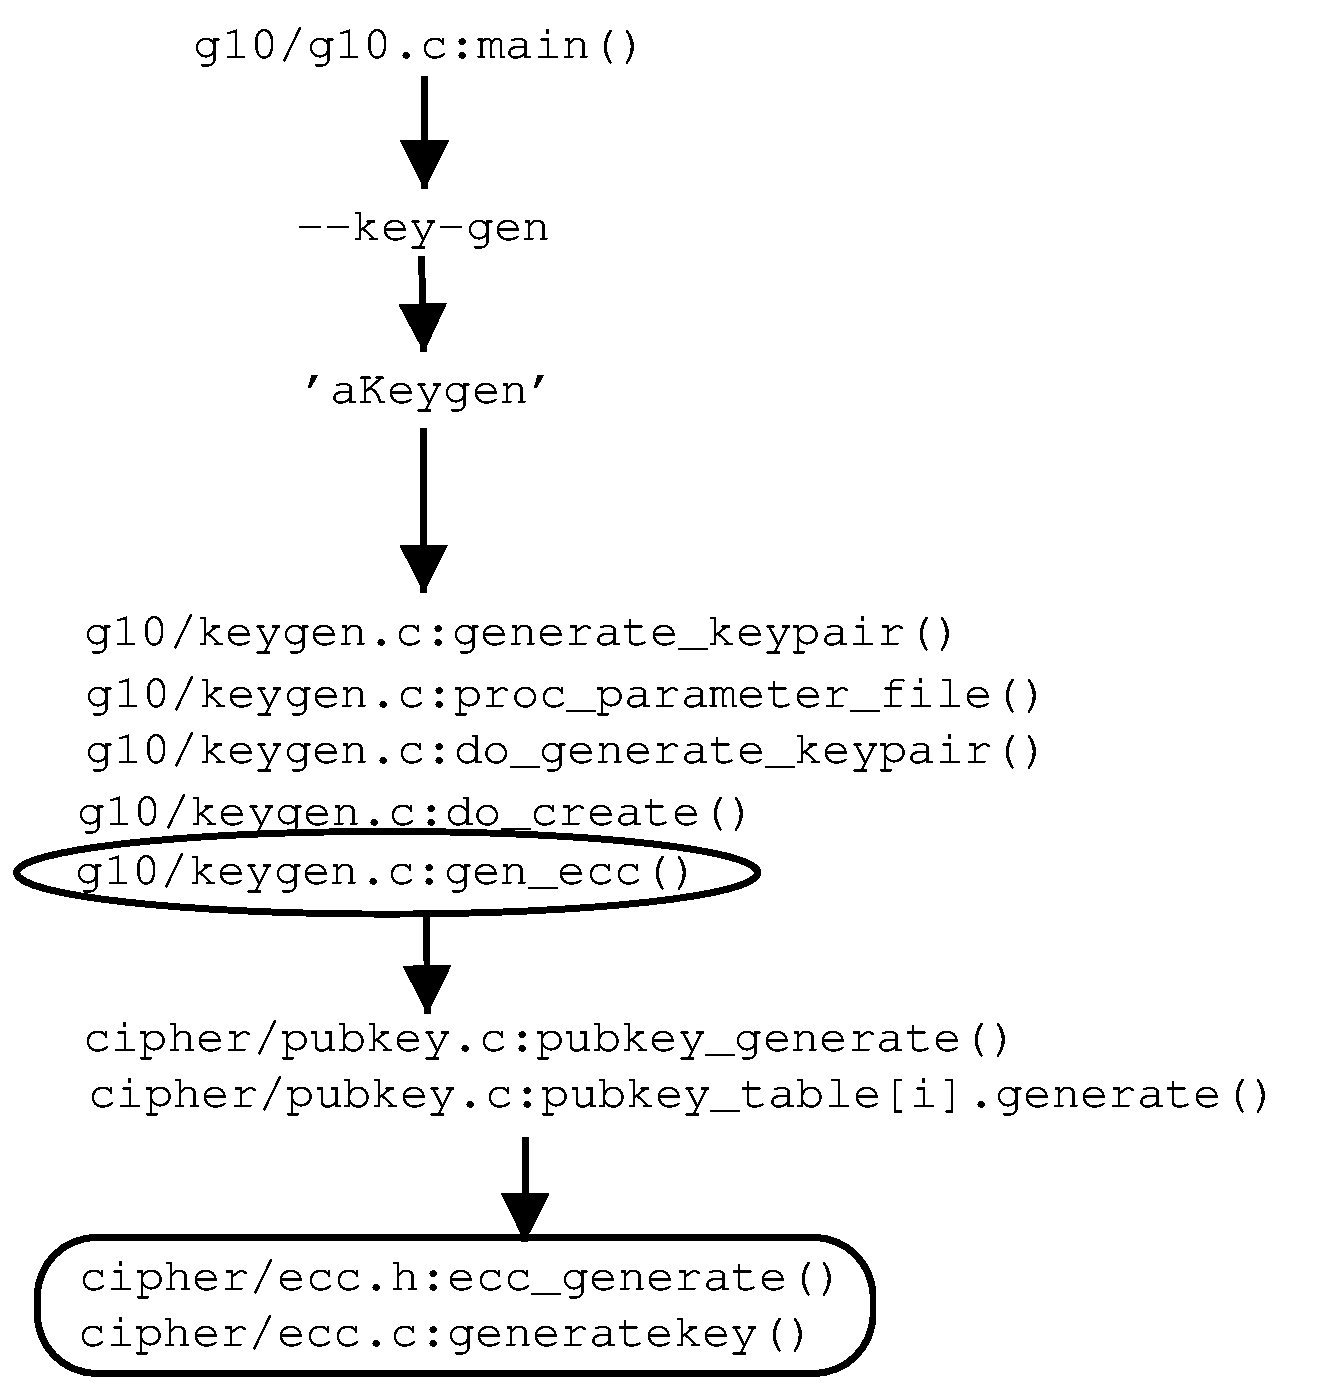
\includegraphics[scale=0.4,keepaspectratio]{./eps/key-gen.eps}
\end{center}
\caption{Scheme of the execution procedure in key generation.}
\end{figure}

\section{Encryption}

In the cipher way, we have two opposite operations to do: Encrypt and Decrypt. The user call this commands with the parameters '\texttt{\$ gpg ----encrypt}' and '\texttt{\$ gpg ----decrypt}', respectively but it is not allow to call both at the same time.

\subsection{Encrypt}

Now we suppose that the use call in the command like the order '\texttt{\$ gpg ----encrypt}', and the program do the same than always: perform the '\texttt{g10/g10.c:main()}' function. The label variable of the command are '\texttt{aEncr}' in this case\footnote{there are other options to encrypt like '\texttt{aEncrFiles}' or '\texttt{aSignEncr}' but the differences are really little, and it is not necessary to make an special mention.}, and the first thing that it do is call the function '\texttt{g10/encode.c:encode\_crypt()}'. The way to go to the ecc module is really near in this case, this function in one step call '\texttt{g10/encode.c:write\_pubkey\_enc\_from\_list()}', but because of the name is not trivial to know that this second function after call '\texttt{cipher/pubkey.c:pubkey\_encrypt()}'. At this point, we jump to the cipher modules directory and we are in the global public key functions; we remember that in the key generation, it use a similar function in this file. Evidently, at this point only rest to find the module interface in the \emph{translation name function table} with the function '\texttt{cipher/pubkey.c:pubkey\_table[i].encrypt}'. This translation guide to the function in the own module interface named '\texttt{cipher/ecc.h:ecc\_encrypt()}' that prepare all the structs to call the private module function '\texttt{cipher/ecc.c:doEncrypt()}'.

\begin{figure}
\begin{center}
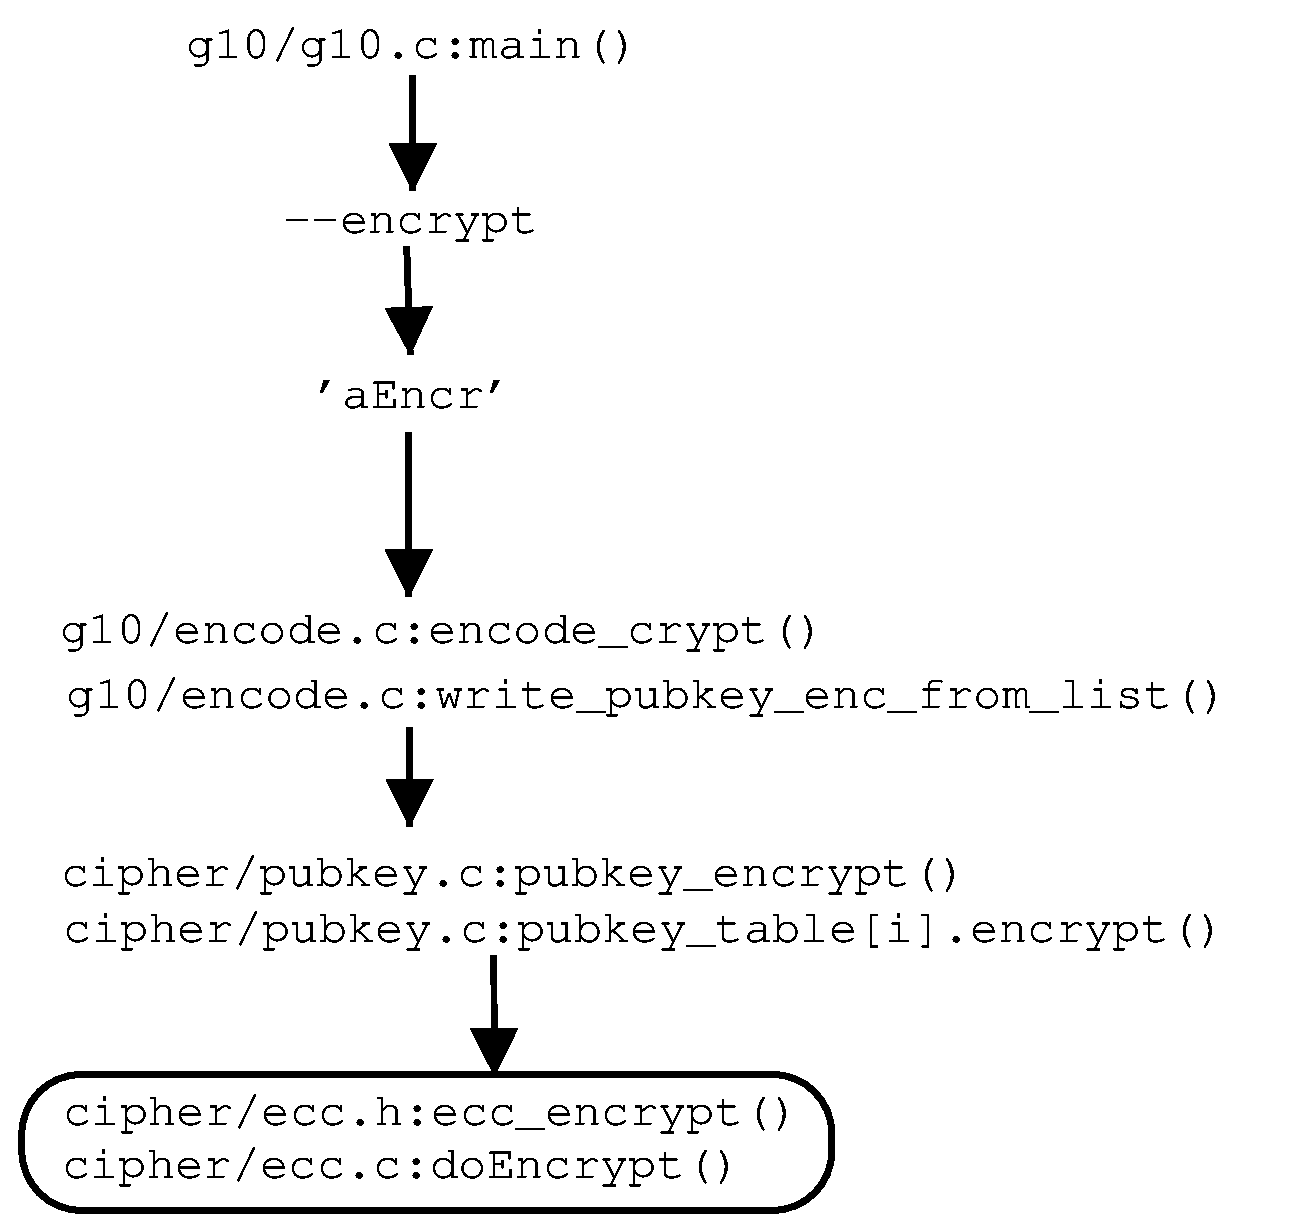
\includegraphics[scale=0.4,keepaspectratio]{./eps/encrypt.eps}
\end{center}
\caption{Scheme of the execution procedure in encryption.}
\end{figure}

\subsection{Decrypt}

In the way to restore the encrypted data, we use the opposite command '\texttt{\$ gpg ----decrypt}', and the program start the execution like always. When the program translate the parameter to the command label variable, named '\texttt{aDecrypt}', call the function '\texttt{g10/decrypt.c:decrypt\_message()}'. In this function, the program control the type of data that it have; for example, if the data have an ascii armor. Then call '\texttt{g10/mainproc.c:proc\_packets()}' to prepare the memory structure and call '\texttt{g10/mainproc.c:do\_proc\_packets()}'. At this time, the program need to know if the data are encrypted with a symmetric algorithm or with a public key one, in the own case is a pubkey and call '\texttt{g10/mainproc.c:proc\_pubkey\_enc()}'. After make different way for the public key algorithms, the program need to know which public key algorithm use, and we can insert the '\texttt{PUBKEY\_ALGO\_ECC}' in the control point, and continue to the '\texttt{g10/pubkey\_enc.c:get\_session\_key()}' and '\texttt{g10/pubkey\_enc.c:get\_it()}' just after, to go to the new module. Now we are in the last points, in the call to the function '\texttt{cipher/pubkey.c:pubkey\_decrypt()}', that access to the translation table '\texttt{cipher/pubkey.c:pubkey\_table[i].decrypt}', to know the interface function '\texttt{cipher/ecc.h:ecc\_decrypt()}', and finally arrive to the own programmed function '\texttt{cipher/ecc.c:decrypt()}'.

\begin{figure}
\begin{center}
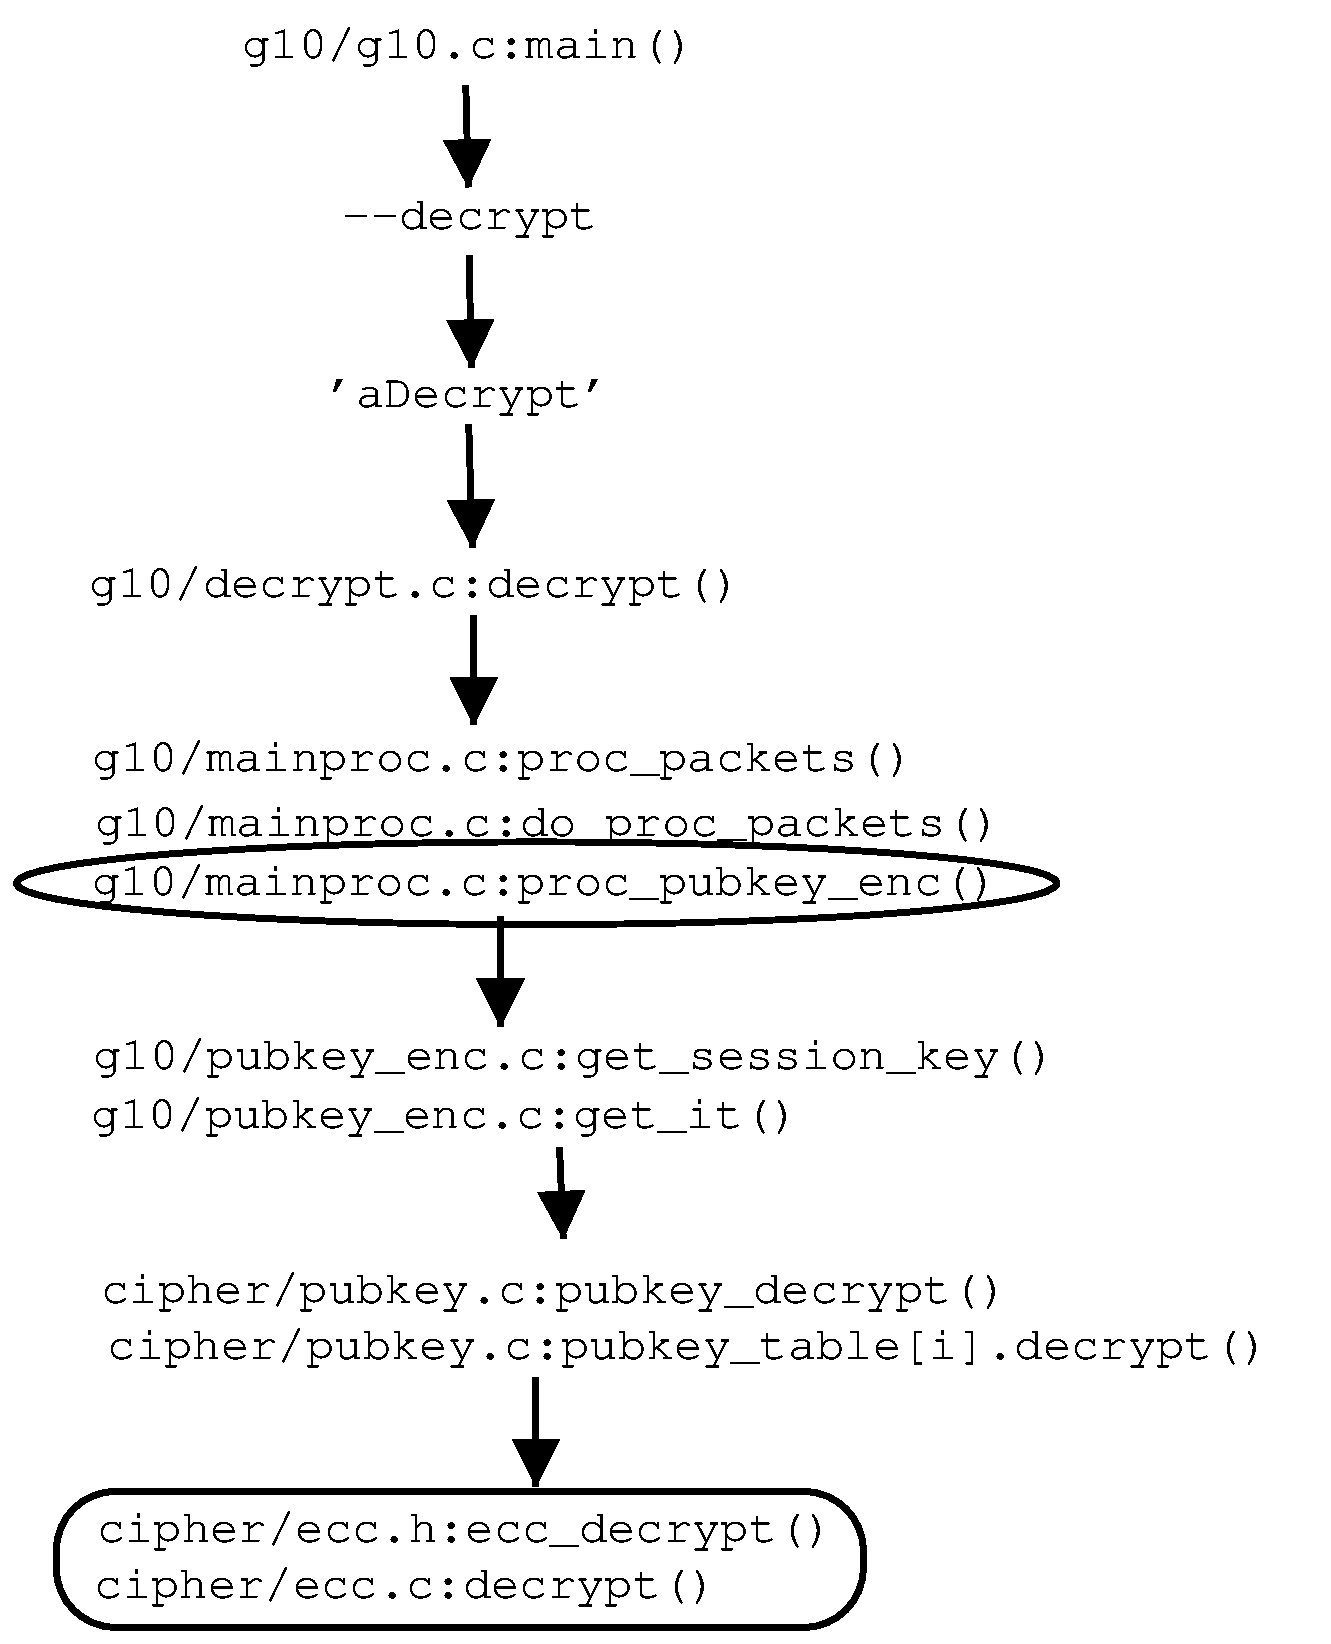
\includegraphics[scale=0.4,keepaspectratio]{./eps/decrypt.eps}
\end{center}
\caption{Scheme of the execution procedure in decryption.}
\end{figure}

\section{Signature}

To make the digital signature and verified if this is correct and nobody make any modification, the user can use the command parameters '\texttt{\$ gpg ----sign}' and '\texttt{\$ gpg ----verify}', now we like to have a description of this procedures.

\subsection{Sign}

The procedure to sign a document is really similar to encrypt in the words of the execution procedure. The first thing is the parameter translation to the command label variable '\texttt{aSign}', and call the function '\texttt{g10/sign.c:sign\_file()}'. The next steps are prepare the blocks and write the sign, and the program do this first with the function '\texttt{g10/sign.c:write\_signature\_packets()}' and then with '\texttt{g10/sign.c:do\_sign()}'. Finally we are in front the modules interface, because of the call to '\texttt{cipher/pubkey.c:pubkey\_sign()}', and the table '\texttt{cipher/pubkey.c:pubkey\_table[i].sign}' that translate the call to the module interface function '\texttt{cipher/ecc.h:ecc\_sign()}'. As the same than in the other commands, at this point only rest to call to the own programmed '\texttt{cipher/ecc.c:sign()}'.

\begin{figure}
\begin{center}
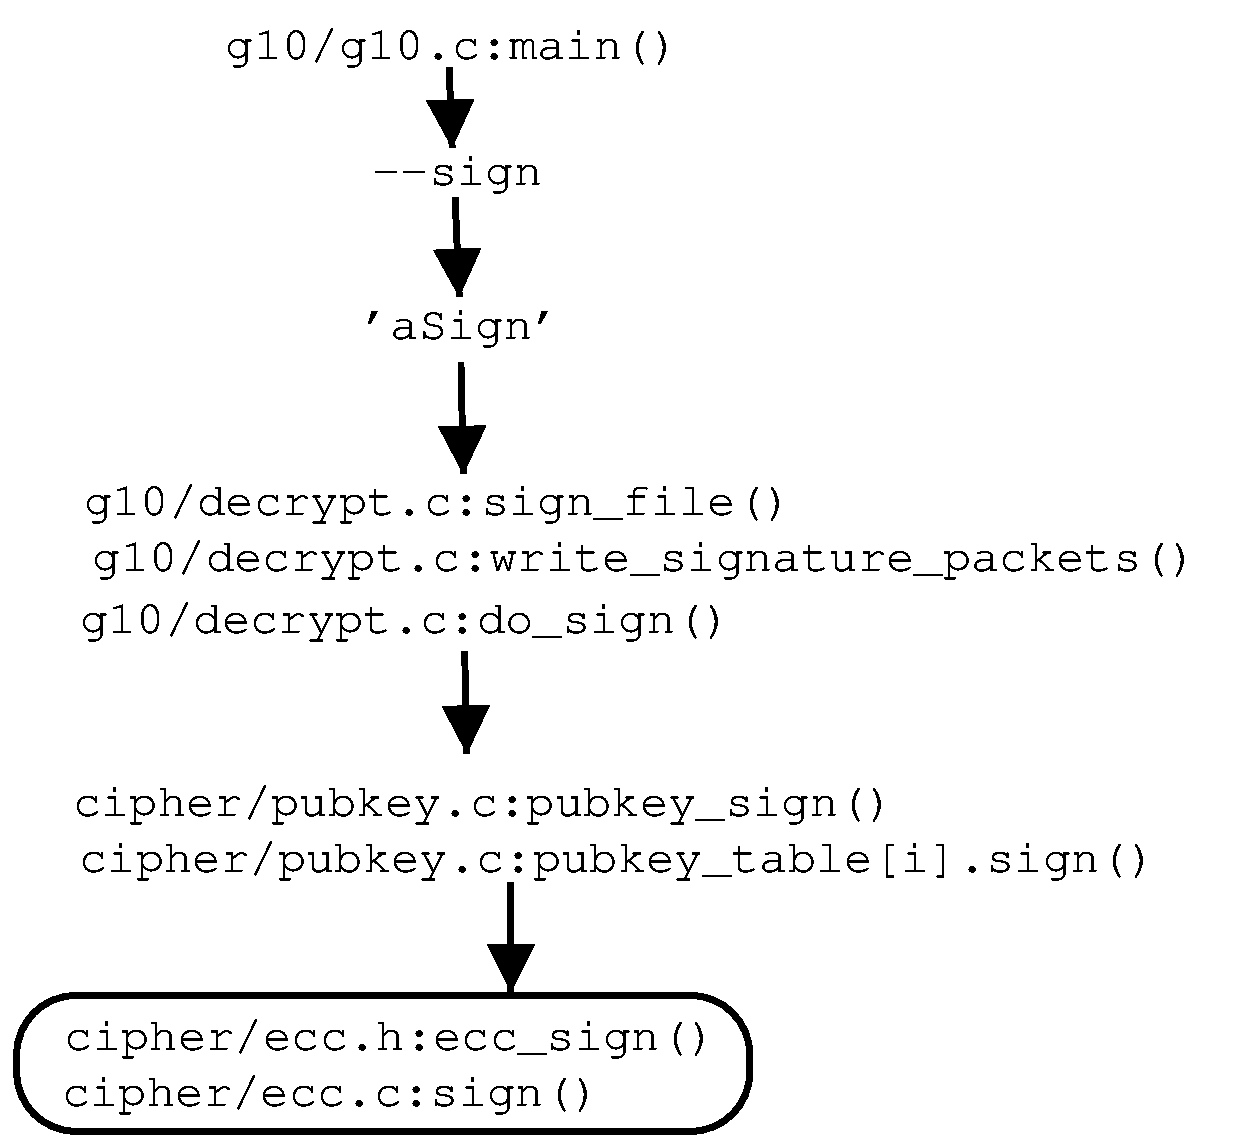
\includegraphics[scale=0.4,keepaspectratio]{./eps/sign.eps}
\end{center}
\caption{Scheme of the execution procedure in the digital signature.}
\end{figure}

\subsection{Verify}

In the last case of the sign verification, there are a lot of functions to call. The parameter translation of the shell command '\texttt{\$ gpg ----verify}', is '\texttt{aVerify}'. The first function to perform is '\texttt{g10/verify.c:verify\_signatures()}', but the next functions are in the '\texttt{g10/mainproc.c}' and it make a lot of jumps into this file ('\texttt{proc\_signature\_packets()}', '\texttt{do\_proc\_packets()}', '\texttt{add\_onepass\_sig()}', '\texttt{release\_list()}', '\texttt{proc\_tree()}', '\texttt{check\_sig\_and\_print()}', '\texttt{do\_check\_sig()}', '\texttt{check\_key\_signature2()}'). After the last one, the program jump to the cipher code section with the call to the function '\texttt{cipher/sig-check.c:signature\_check2()}' and the function '\texttt{cipher/sig-check.c:do\_check()}'. Finally we are at the modules inteface with the call '\texttt{cipher/pubkey.c:pubkey\_verify()}', and the translation in the table '\texttt{cipher/pubkey.c:pubkey\_table[i].verify}', and go to the module calling '\texttt{cipher/ecc.h:ecc\_verify()}'. The function in the own module to verify one signature, that it is called from the module interface is '\texttt{cipher/ecc.c:verify()}'.

\begin{figure}
\begin{center}
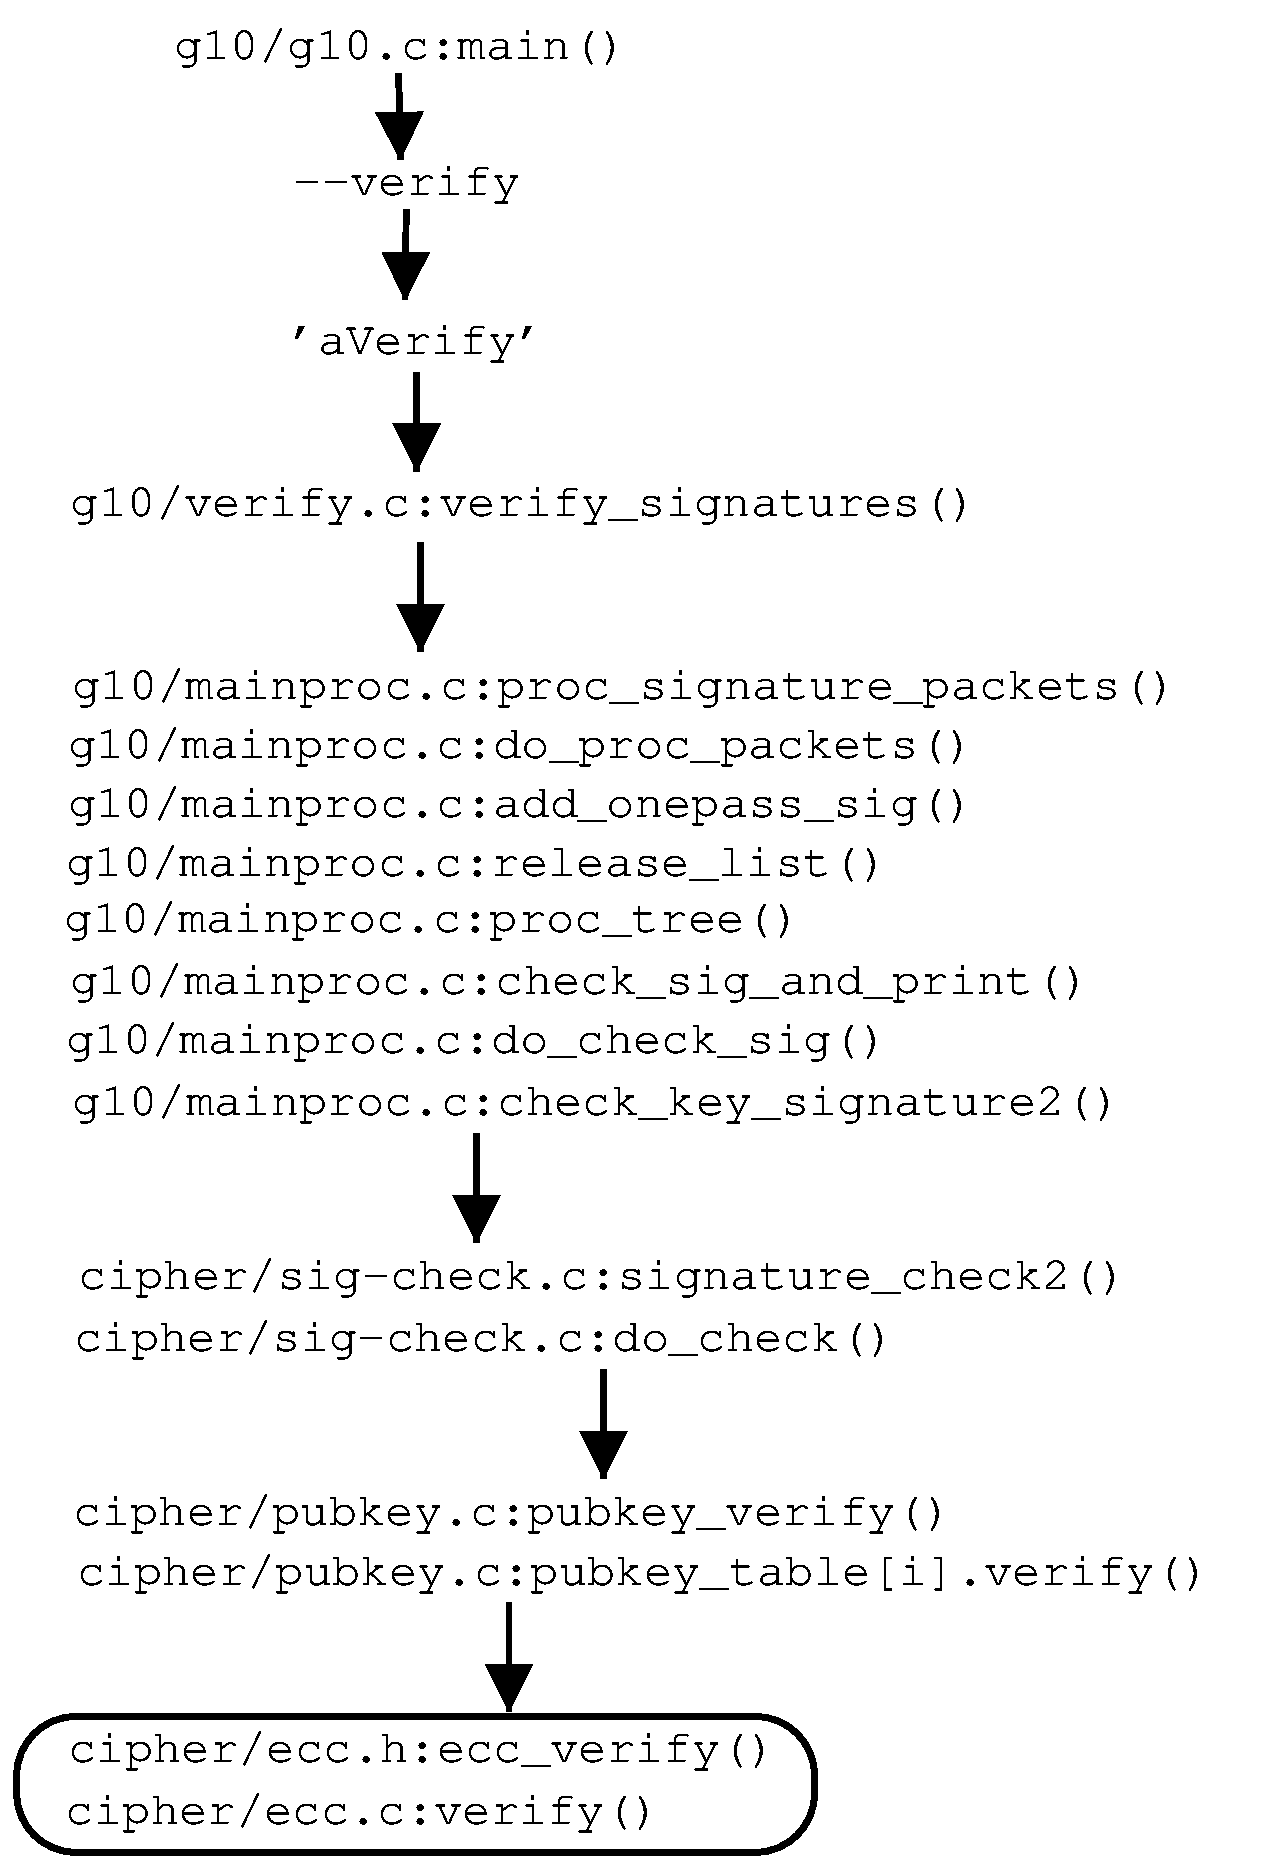
\includegraphics[scale=0.4,keepaspectratio]{./eps/verify.eps}
\end{center}
\caption{Scheme of the execution procedure in the signature verification.}
\end{figure}


\begin{figure}
\begin{center}
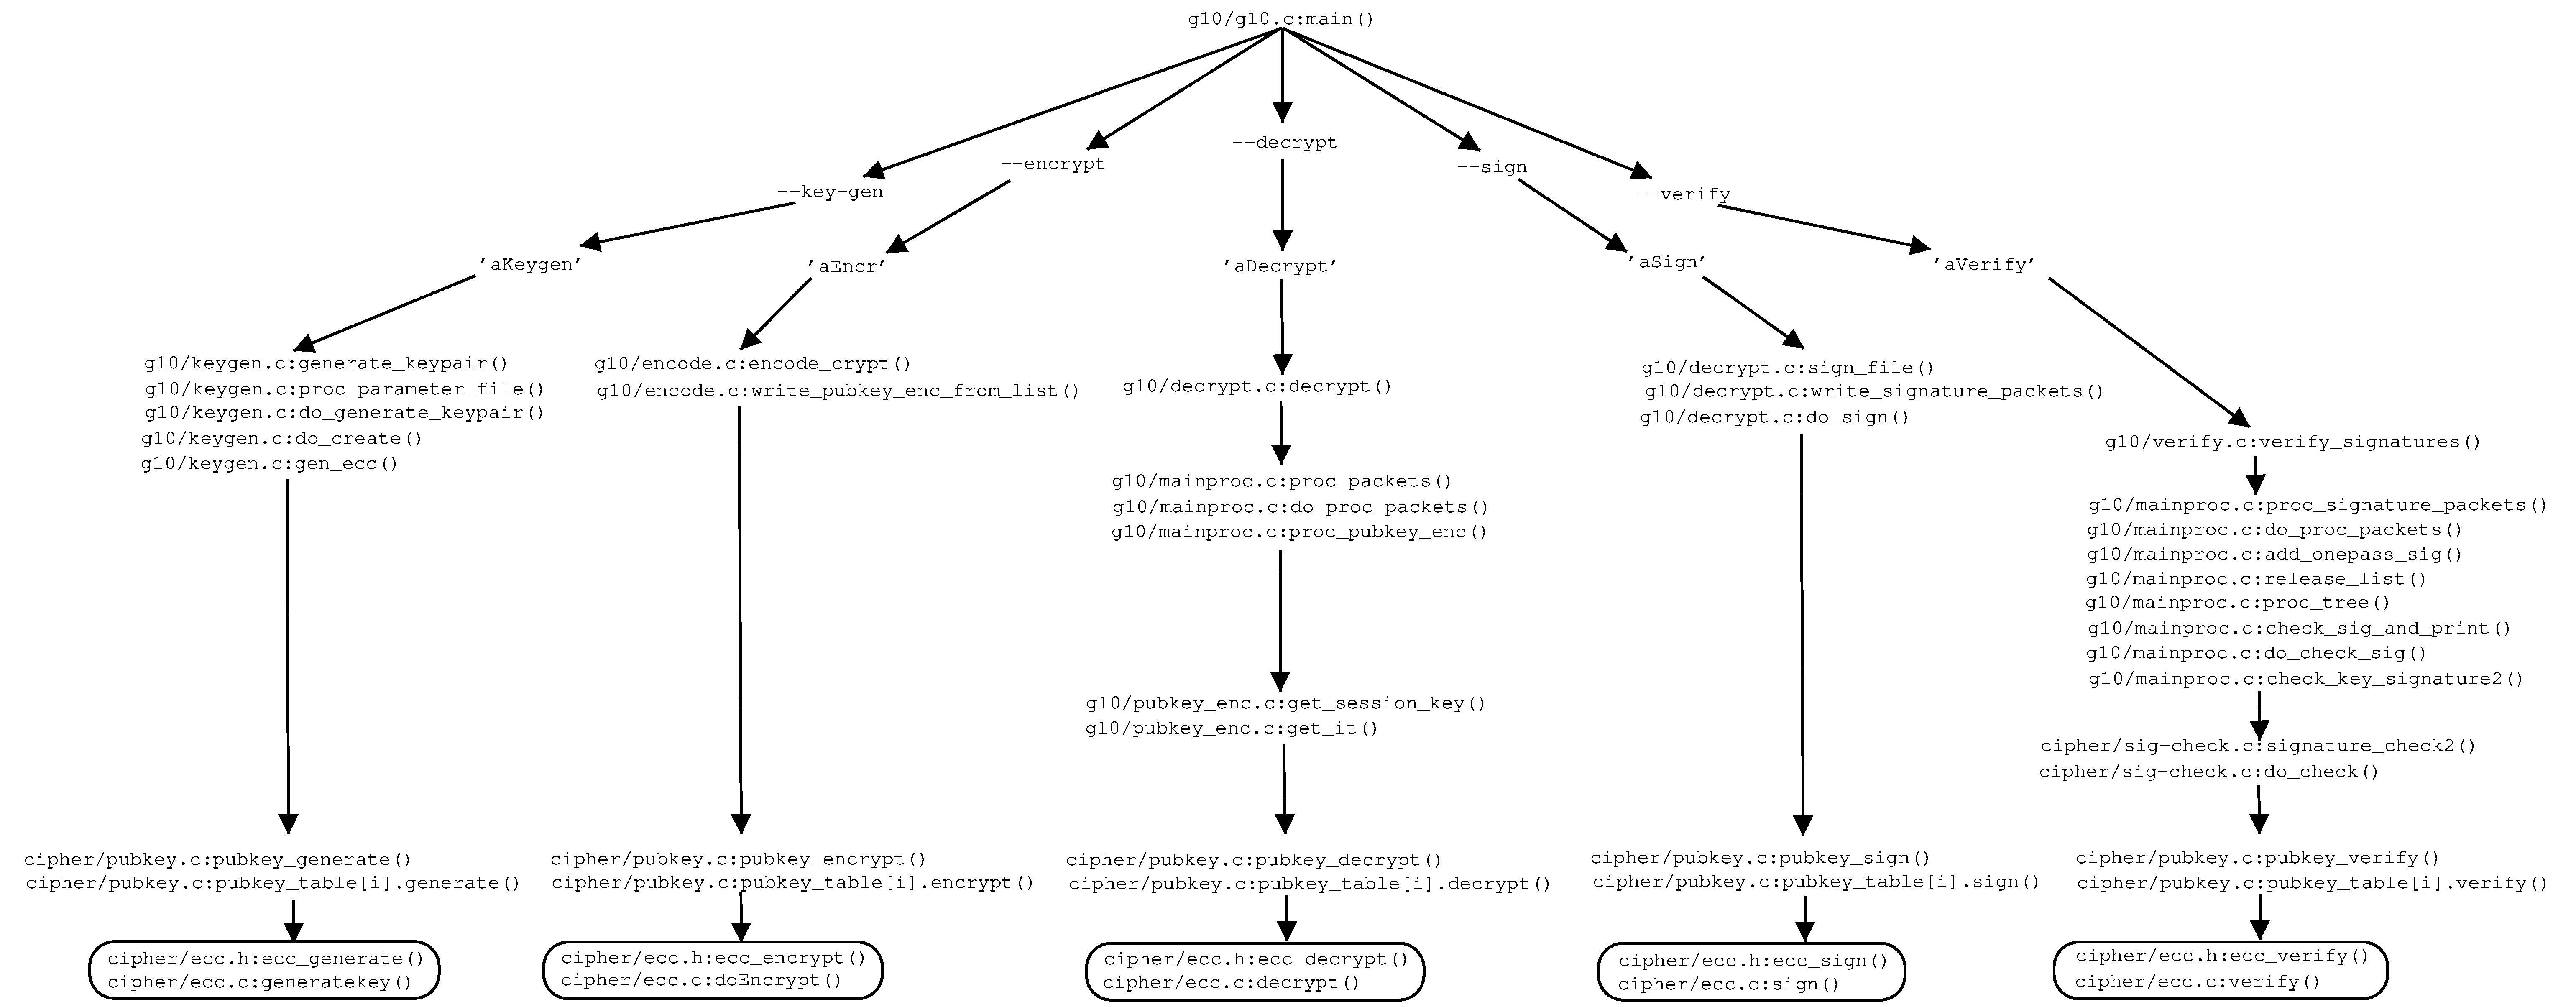
\includegraphics[scale=0.2,keepaspectratio,angle=90]{./eps/apendixc.eps}
\end{center}
\caption{Global scheme of the execution procedure in this work.}
\end{figure}

\begin{thebibliography}{1}
\bibitem[P1363]{P1363}IEEE P1363/D13 (Draft Version 13) Standard Specifications for Public key Cryptography. 1999 November 12.
\bibitem[NIST]{NIST}FIPS PUB 186-2, Digital Signature Standard (DSS), U.S.Department of Commerce/National Institute of Standards and Technology. 2000 January 27.
\bibitem[Auto98]{conf}Autoconf:Creating Automatic Configuration Scripts. Edition 2.13, for Autoconf version 2.13. December 1998
\bibitem [822] {rfc822}Standard for the format of arpa internet text messages (Obsolete: see 2822). 1982 August.
\bibitem[1991]{rfc1991}PGP Message Exchange Formats. 1996 August.
\bibitem[2015]{rfc2015}MIME Security with Pretty Good Privacy (PGP) (Obsolete: see 3156). 1996 October.
\bibitem[2440]{rfc2440}OpenPGP Message Format. 1998 November
\bibitem[2822]{rfc2822}Internet Message Format. 2001 April.
\bibitem[3156]{rfc3156}MIME Security with OpenPGP. 2001 August.
\bibitem[3278]{rfc3278}Use of Elliptic Curve Cryptography (ECC) Algorithms in Cryptographic Message Syntax (CMS). 2002 April.
\bibitem[PKCS\#1]{PKCS}PKCS\#1 v2.1: RSA Crptography Standard. RSA Laboratories. 2002 June 14.
\bibitem[mov97]{handbook} Alfred J, Menezes, Paul C.van Oorschot, and Scott A. Vanstone. \textit{Handbook of Applied Cryptography}. CRC Press, first edition, 1997. http://cacr.math.uwaterloo.ca/hac/
\bibitem[WZ99]{WZ99}M.Wiener and R. Zuccherato, \textit{Faster attacks on elliptic curve cryptosystems}, Selected Areas in cryptography, Lecture notes in Computer Science, n1556 (1999), Springer-Verlag, 190-200.
\bibitem[PH78]{PH78}S. Pohlig and M. Hellman, \textit{An improved algorithm for computing logarithms over GF(p) and its cryptographic significance}, IEEE Transactions on Information Theory, n24 (1978), 106-110.
\bibitem[OW99]{OW99}P. Van Oorschot and M. Wiener, \textit{Parallel Collision search with cryptanalytic applications}, Journal of Cryptology, n12 (1999), 1-28.
\bibitem[Mill86]{Mill86}V. Miller, \textit{uses of elliptic curves in cryptography}l Advances in Cryptology - Crypto '85, Lecture Notes in Computer Science, n218 (1986), Springer-Verlag, 417-426.
\bibitem[Silv99]{Silv99}J. Silverman and J. Suzuki, \textit{Elliptic curve discrete logarithms and the index calculus}, advances in Cryptology - Asiacrypt '98, Lecture Notes in Computer Science, n1514 (1999), Springer-Verlag, 110-125.
\bibitem[Silv00]{Silv00}J. Silverman, \textit{The Xedni calculus and the elliptic curve discrete logarithm problem}, Designs, codes and Cyptography, n20 (2000), 5-40.
\bibitem[Men95]{Men95}Alfred Menezes, \textit{Elliptic curve Cryptosystems}, CryptoBytes - The Technical Newsletter of RSA Laboratories, volumen 1, number 2, Summer 1995, 1-4.
\bibitem[Xedni99]{Xedni99}M. j. jacobson, N. Koblitz, J. H. Silverman, A. Stein, E. Teske, \textit{Analysis of the Xedni Calculus Attack}, 1999.
\bibitem[ECDSA]{JMV}D. Johnson, A. Menezes, S. Vanstone, \textit{The elliptic Curve Digital Signature Algorithm (ECDSA)}. Dept. of Combinatorics \& Optimization, University of Waterloo, Certicom, Canada.
\bibitem[Men93]{Men93}Alfred Menezes, \textit{Elliptic Curve Public Key Cryptosystems}. Kluwer Academic Publishers, 1993
\bibitem[Rami02]{Rami02}Manuel Rami Perat, \textit{Factorizaci\'on con curvas el\'ipticas. Variantes del algoritmo de Lenstra.} TFC (director: Josep Maria Miret Biosca), EUP UdL, Gener 2002.
\bibitem[Cosi01]{Cosi01}Ana Cosialls Abill\'a, \textit{Criptosistemas tipo el ElGamal con curvas el\'ipticas.} TFC (directora: Magda Valls Marsal), EUP UdL, Febrer 2001.
\bibitem[toolstut]{autotools_tutorial}Eleftherios Gkioulekas \textit{Learning the GNU development tools}. 1998-07-29. Edition 1
\bibitem[autoconf]{autoconf_tutorial}Mark Galassi \textit{Autoconf Tutorial}
\bibitem[toolsman]{autoconf_manual}David MacKenzie and Ben Elliston \textit{Autoconf, Creating Automatic Configuration Scripts}. December 1998. Edition 2.13, for Autoconf version 2.13
%IFP ElGamal Weakness:
\bibitem[DJN]{DJN}Dan Doneh, Antoine Joux, Phong Q. Nguyen \textit{Why Textbook ElGamal and RSA Encryption are Insecure}. Extended Abstract.
\bibitem[DHAES]{DHAES} Michel Abdalla, Mihir Bellare, Phillip Rogeway \textit{DHAES: An Exncryption Scheme Based on the Diffie-Hellman Problem}. September 1998. Submission to IEEE P1363a.
\bibitem[EPOC]{EPOC} Tatsuaki Okamoto, Shigenori Uchiyama, Eiichiro Fujisaki \textit{EPOC: Efficient Probabilistic Public-Key Encryption}. November 1998. Submission to IEEE P1363a.
\bibitem[EPOC3]{EPOC3} Tatsuaki Okamoto, David Pointcheval \textit{EPOC-3: Efficient Probabilistic Public-key Encryption - v3}. May 2000. Submission to P1363a.
\bibitem[P1363a]{P1363a} Tatsuaki Okamoto \textit{Proposal to IEEE P1363a}. February 2000.
\bibitem[SEC1]{SEC1} Dan Boneh \textit{Review ofSEC1: Elliptic Curve Cryptography}.
%fi
\end{thebibliography}

\end{document}

